%%%%%%%%%%%%%%%%%%%%%%%%%%%%%%%%%%%%%%%%%%%%%%%%%
% Vorlage für Abschlussarbeiten
% Fachgebiet Regelungsmethoden und Robotik
% v1.6, 24.07.2018
%%%%%%%%%%%%%%%%%%%%%%%%%%%%%%%%%%%%%%%%%%%%%%%%%
% Hauptdatei der LaTeX-Vorlage
%
% Kompiler: pdflatex oder latex > dvips > ps2pdf
% Zeichenkodierung: UTF-8
%%%%%%%%%%%%%%%%%%%%%%%%%%%%%%%%%%%%%%%%%%%%%%%%%
\documentclass[a4paper,            	% Papierformat
               12pt,               	% Schriftgr\"{o}{\ss}e
               chapterprefix,      	% Wort "chapter" in Kapitel\"{u}berschrift
               appendixprefix,		% Wort ``Anhang'' vor den Anhangskapiteln
               headsepline,        	% Trennlinie zwischen Kopf und Text
%                oneside,           % einseitiges Dokument
               twoside,				% oder zweiseitig
               %pointlessnumbers, 	% Nummerierung ohne Punkte am Ende z.B. 1.3
               %bigheadings,		% Größe der Überschriften
               draft=false]         % Ausschalten der Fehleranzeige
               {scrbook}			% wir schreiben ein Buch (KOMA-Buch)
\usepackage[utf8]{inputenc}			% Quelltext UTF-8 kodiert

\makeatletter
\if@twoside
	\setlength{\oddsidemargin}{6mm}
	\setlength{\evensidemargin}{-6mm}
\fi


%%%%%%%%%%%%%%%%%%%%%%%%%%%%%%%%%%%%%%%%%%%%%%%%%
%------ vordefinierte Variablen --------
% (mit eigenen Angaben füllen!)
%%%%%%%%%%%%%%%%%%%%%%%%%%%%%%%%%%%%%%%%%%%%%%%%%
\newcommand{\BaMaType}{Bachelor Thesis}  % Bachelor-Thesis oder Master-Thesis
\newcommand{\BaMaAuthor}{Runchida Kaewngoen}  % Name des Verfassers
\newcommand{\BaMaProgramme}{Studiengang Elektrotechnik und Informationstechnik}	 % Studiengang
\newcommand{\BaMaTitle}{Survey on Image Classification in the Domain Mixture Scenario}  % Titel der Arbeit
\newcommand{\BaMaFinishDate}{10.02.2020}  % Einreichungsdatum der Arbeit
\newcommand{\BaMaSupervisor}{Sebastian Schrom, M.Sc.} % Betreuer (Wissenschaftlicher Mitarbeiter)


%%%%%%%%%%%%%%%%%%%%%%%%%%%%%%%%%%%%%%%%%%%%%%%%%
% Defintion Referenzen
%%%%%%%%%%%%%%%%%%%%%%%%%%%%%%%%%%%%%%%%%%%%%%%%%
\newcommand{\figref}[1]{Abb. \ref{#1}}
\newcommand{\thmref}[1]{Satz \ref{#1}}
\newcommand{\chref}[1]{Kapitel \ref{#1}}
\newcommand{\secref}[1]{Abschnitt \ref{#1}}
\newcommand{\tabref}[1]{Tabelle \ref{#1}}
\newcommand{\defref}[1]{Definition \ref{#1}}
\newcommand{\bspref}[1]{Bsp. \ref{#1}}
\newcommand{\corref}[1]{Korollar \ref{#1}}


%%%%%%%%%%%%%%%%%%%%%%%%%%%%%%%%%%%%%%%%%%%%%%%%%
% BaMa-Header (Deutsch/Englisch)
%%%%%%%%%%%%%%%%%%%%%%%%%%%%%%%%%%%%%%%%%%%%%%%%%
% => include 'BaMa_Header_english' instead of 'BaMa_Header_deutsch' if you write in your thesis in english!
%%%%%%%%%%%%%%%%%%%%%%%%%%%%%%%%%%%%%%%%%%%%%%%%%%%%%%%%%%%%
% Header-Datei mit sprachspezifischen Einstellungen        %
% (english version)                                        %
%%%%%%%%%%%%%%%%%%%%%%%%%%%%%%%%%%%%%%%%%%%%%%%%%%%%%%%%%%%%


% english terms for preamble
\newcommand{\SupervisorString}{Supervisor}
\newcommand{\AcknowledgementString}{Acknowledgement}

% english translation of 'Selbständigkeitserklärung'
\newcommand{\EEoptionalTranlation}{%
		\vspace*{5\baselineskip}
		{\small\bfseries\sffamily (English translation of above declaration for information purposes only)\\[0.5\baselineskip]
		{Thesis Statement\\pursuant to § 22 paragraph 7 and § 23 paragraph 7 of APB TU Darmstadt}}\\[0.5\baselineskip]
		I herewith formally declare that I, \BaMaAuthor{}, have written the submitted \BaMaType{} independently pursuant to § 22 paragraph 7 of APB TU Darmstadt. I did not use any outside support except for the quoted literature and other sources mentioned in the paper. I clearly marked and separately listed all of the literature and all of the other sources which I employed when producing this academic work, either literally or in content. This thesis has not been handed in or published before in the same or similar form.
		I am aware, that in case of an attempt at deception based on plagiarism (§38 paragraph 2 APB), the thesis would be graded with 5,0 and counted as one failed examination attempt. The thesis may only be repeated once.

		In the submitted thesis the written copies and the electronic version for archiving are pursuant to § 23 paragraph 7 of APB identical in content.%
	}
	% Header mit sprachspezifischen Voreinstellungen
%%%%%%%%%%%%%%%%%%%%%%%%%%%%%%%%%%%%%%%%%%%%%%%%%%%%%%%%%%%%
% Header-Datei zur Erstellung einer BaMa am Fachgebiet rmr %
%%%%%%%%%%%%%%%%%%%%%%%%%%%%%%%%%%%%%%%%%%%%%%%%%%%%%%%%%%%%
% Diese Datei definiert alle wichtigen Sachen, so dass sich die Studenten nur noch mit dem Schreiben der Arbeit beschäftigen können, wenn diese Datei genutzt wird. Die Nutzung ist natürlich keine Pflicht aber empfohlen!


%%%%%%%%%%%%%%%%%%%%%%%%%%%%%%%%%%
%------------- Pakete ------------
%%%%%%%%%%%%%%%%%%%%%%%%%%%%%%%%%%
% Schrift & Sprache
\usepackage[T1]{fontenc}			% Darstellung von Schrift als echte T1 Fonts und nicht als Bilder
\usepackage{lmodern}				% hübsche Schrift, kein Pixelmatsch

% Layout & Struktur
\usepackage[automark,autooneside]{scrpage2}	% KOMA-Paket für Seitenlayout
\usepackage{calc}					% Satzspiegelberechnung (Texthöhe zu Textbreite usw.)
\usepackage[numbers]{natbib}
\usepackage[small]{caption}
\usepackage{float}
\usepackage{nomencl}
\usepackage{lscape}
\usepackage{textcomp}

% Mathematik & Formeln
\usepackage{amsmath}				% Mathematik-Umgebungen
\usepackage{amssymb}				% spezielle Mathe-Symbole
\usepackage{amsthm}
\usepackage{amsfonts}
\usepackage{bm}						% fette Mathe Buchstaben
\usepackage{delarray}
\usepackage{dsfont}					% spezielle Mathe-Buchstaben (z.B. Mengenzeichen)
\usepackage{bbm}					% weitere spezielle Mathe-Buchstaben (z.B. Mengenzeichen)
\usepackage{algorithmic}
\usepackage{empheq}
\usepackage{commath}				% nützliche Mathe-Makros

% Grafiken & Farbe
\usepackage{graphicx}				% zum einbinden von Grafiken
\usepackage{xcolor}					% für Farben und Farbdefinitionen
\usepackage{tikz,pgfplots}
\usetikzlibrary{arrows,fit,backgrounds,shapes.arrows,decorations.pathmorphing}
%\usepackage{psfrag}				% zum Verändern / Ersetzen von Text in Grafiken
%\usepackage{pstricks}				% Zeichnen mit LaTeX
%\usepackage{thmbox}
%\usepackage{shadethm}
%\usepackage{enumitem}

% Hyperlinks im PDF
\usepackage[
			colorlinks,     	% farbige Links
            linkcolor=black,	% allg. Linkfarbe
            citecolor=black,	% Farbe für Literaturstellen
            urlcolor=black,		% Farbe für Websites
            linktocpage,        % nur die Seite des Inhaltsverzeichnis wird verlinkt
            bookmarksopen]      % Lesezeichen im Adobe Reader auf für alle Kapitel, Unterkapitel usw.
	{hyperref}


%%%%%%%%%%%%%%%%%%%%%%%%%%%%%%%%%%%%%%%%%%%%%%%%%
%=========== KOMA Befehle (Layout) ==============
%%%%%%%%%%%%%%%%%%%%%%%%%%%%%%%%%%%%%%%%%%%%%%%%%
\pagestyle{scrheadings}                             	% KOMA-Headings benutzen
\clearscrheadfoot                           			% alle Felder im Kopf und Fuß löschen
\renewcommand{\headfont}{\normalfont\small\sffamily\bfseries}
\renewcommand{\pnumfont}{\normalfont\small\sffamily\bfseries }	
\renewcommand*{\chaptermarkformat}{\thechapter\autodot\enskip}	% kein chapterprefix in der Kopfzeile
\automark[section]{section}                         	% aktuelle section als Kolumnentitel
\lohead{\headmark}                                  	% links oben steht dieser Kolumnentitel, auf ungeraden Seiten
\lehead{\pagemark}                                  	% links oben Seitenzahl auf geraden Seiten
\cfoot[\pagemark]{}										% Seitennummer unten zentriert, wenn keine Kolumnentitel
\rehead{\headmark}										% rechts oben steht der Kolumnentitel, auf geraden Seiten
\rohead{\pagemark}										% rechts oben Seitenzahl auf ungeraden Seiten
\setheadsepline{0.5pt}                              	% Trennlinie zwischen Kopfzeile und Text mit 0.5pt Dicke


%%%%%%%%%%%%%%%%%%%%%%%%%%%%%%%%%%%%%%%%%%%%%%%%%
%-------------Pfad für die Logos-----------------
%%%%%%%%%%%%%%%%%%%%%%%%%%%%%%%%%%%%%%%%%%%%%%%%%
\graphicspath{{./logos/}}


%%%%%%%%%%%%%%%%%%%%%%%%%%%%%%%%%%%%
%---------- Titel ------------------
%%%%%%%%%%%%%%%%%%%%%%%%%%%%%%%%%%%%
\definecolor{rmrGruen}{rgb}{0.6,0.753,0}	% rmr-Grün (hier aber nicht benutzt)

\titlehead{ % Kopf der Titelseite
	\vspace{-2cm}
	\parbox[b]{80mm}{\huge\sffamily\bfseries \BaMaType}
	\hfill
	\parbox[b]{90mm}{
\includegraphics[scale=0.35]{TUD}}\vspace{0.15cm}
	\rule{\textwidth}{2pt} }
 
\subject{\vspace{30mm}}	% Betreff der Titelseite (hier leer)

\title{\BaMaTitle} % Titel der Arbeit

\author{\BaMaAuthor\\[6pt]\BaMaProgramme} % Autor der Arbeit + Studiengang

\date{ \vspace{\baselineskip}\BaMaFinishDate\vspace{40mm}} % Einreichungsdatum der Arbeit

\publishers{ % Fuß der Titelseite
	\rule{\textwidth}{2pt}\\[0.5\baselineskip]
	\parbox[b]{75mm}{\sffamily \SupervisorString{}: \\ \BaMaSupervisor}
	\hfill
	\parbox[b]{68mm}{
\includegraphics[scale=1.5]{rmr}\\ \raggedleft\textsf{Prof. Dr.-Ing. J. Adamy}}
	\vspace{-30mm}}

\dedication{ % Selbständigkeitserklärung
	\normalfont\normalsize\thispagestyle{plain}
	\begin{minipage}[t][0.95\textheight][t]{\textwidth}
		{\huge\bfseries\sffamily Eidesstattliche Erklärung}\\[0.2\baselineskip]
		{\small\bfseries\sffamily Erklärung zur Abschlussarbeit gemäß § 22 Abs. 7 und § 23 Abs. 7 APB TU Darmstadt} \\[0.5\baselineskip]
		
		Hiermit versichere ich, \BaMaAuthor{}, die vorliegende \BaMaType{} gemäß § 22 Abs.~7 APB der TU Darmstadt ohne Hilfe Dritter und nur mit den angegebenen Quellen und Hilfsmitteln angefertigt zu haben. Alle Stellen, die Quellen entnommen wurden, sind als solche kenntlich gemacht worden. Diese Arbeit hat in gleicher oder ähnlicher Form noch keiner Prüfungsbehörde vorgelegen.
		Mir ist bekannt, dass im Falle eines Plagiats (§38 Abs.~2 APB) ein Täuschungsversuch vorliegt, der dazu führt, dass die Arbeit mit 5{,}0 bewertet und damit ein Prüfungsversuch verbraucht wird. Abschlussarbeiten dürfen nur einmal wiederholt werden.
		
		Bei der abgegebenen Thesis stimmen die schriftliche und die zur Archivierung eingereichte elektronische Fassung gemäß § 23 Abs. 7 APB überein.\\[1.5\baselineskip]
		\noindent Darmstadt, \BaMaFinishDate   \\[2\baselineskip]
		\noindent \BaMaAuthor

		\EEoptionalTranlation
	\end{minipage}}


%%%%%%%%%%%%%%%%%%%%%%%%%%%%%%%%%%%%%%%%
%-------------- Umgebungen -------------
%%%%%%%%%%%%%%%%%%%%%%%%%%%%%%%%%%%%%%%%

% Umgebung zum Setzen des Abstract und der Zusammenfassung
\newenvironment{BaMaAbstract}[2]{
	\thispagestyle{plain}
	\begin{minipage}[c][\textheight][c]{\textwidth}
	\begin{center}\huge\bfseries\sffamily
		Abstract
	\end{center}
	\normalfont
	#1
	\\[0.1\baselineskip]
	\begin{center}
	\rule{0.5\textwidth}{0.5pt}
	\end{center}
	\begin{center}\huge\bfseries\sffamily
		Zusammenfassung
	\end{center}
	\normalfont
	#2
}{
	\end{minipage}\newpage
}


% Umgebung zum Setzen der Danksagung
\newenvironment{BaMaAcknowledgements}[1]{ 
	\cleardoublepage
	\thispagestyle{plain}
	\begin{minipage}[c][\textheight][t]{\textwidth}
	 {\noindent\huge\bfseries\sffamily \AcknowledgementString}\\[\baselineskip]
	 \normalfont
	 #1
	 \\[1\baselineskip]
	 \noindent\BaMaAuthor
}{
	\end{minipage}\newpage
}


%%%%%%%%%%%%%%%%%%%%%%%%%%%%%%%%%%%%%%%%%%%%%%%%%
% Anpassung Abkürzungsverzeichnis
%%%%%%%%%%%%%%%%%%%%%%%%%%%%%%%%%%%%%%%%%%%%%%%%%

% Befehl umbenennen in \abk
\let\abk\nomenclature

% Überschriften anpassen
\renewcommand{\nomname}{Verzeichnis der verwendeten Abkürzungen und Formelzeichen}
\RequirePackage{ifthen}
\renewcommand{\nomgroup}[1]{%
	\ifthenelse{\equal{#1}{A}}{\item[\textbf{Abkürzungen}]}{%
		\ifthenelse{\equal{#1}{F}}{\bigskip\item[\textbf{Formelzeichen}]}{}}{}}

% Formatierung Abkürzungsverzeichnis anpassen
\setlength{\nomlabelwidth}{.15\hsize} % Abstand zw. Abkürzung und Erklärung anpassen
%\setlength{\nomitemsep}{-3.5pt} % Zeilenabstände verkleinern


%%%%%%%%%%%%%%%%%%%%%%%%%%%%%%%%%%%%%%%%%%%%%%%%%%
% Konfiguration Float-Platzierung
%%%%%%%%%%%%%%%%%%%%%%%%%%%%%%%%%%%%%%%%%%%%%%%%%%
% Dies Parameter steuern die Platzierung von figure, table, usw.
% Falls nötig aktivieren und anpassen. Das ist oft besser als die Platzierung zu erzwingen.
%%%%%%%%%%%%%%%%%%%%%%%%%%%%%%%%%%%%%%%%%%%%%%%%%%
%\renewcommand{\topfraction}{0.5}     % maximaler Platzanteil im oberen Teil einer Seite für Floats
%\renewcommand{\bottomfraction}{0.5}  % maximaler Platzanteil im untern Teil einer Seite für Floats
%\renewcommand{\textfraction}{0.5}    % minimaler Platzanteil für Text
%\setcounter{topnumber}{2}            % maximale Anzahl an Floats im oberen Teil einer Seite
%\setcounter{bottomnumber}{2}         % maximale Anzahl an Floats im unteren Teil einer Seite
%\setcounter{totalnumber}{3}          % maximale Anzahl an Floats auf einer Seite insgesamt
		% Header mit den wichtigen Voreinstellungen laden - NICHT ÄNDERN!!!!!
                            	% => alle BaMa sehen gleich aus.


%%%%%%%%%%%%%%%%%%%%%%%%%%%%%%%%%%%%%%%%%%%%%%%%%%
% Styles für mathematische Definitionen etc.     
% (kann natürlich angepasst werden!)             
%%%%%%%%%%%%%%%%%%%%%%%%%%%%%%%%%%%%%%%%%%%%%%%%%%

% Definitionen, Sätze, Beispiele, Beweise (ohne THMBOX)
\newtheoremstyle{defstyle}
	{9pt}									% space above
	{9pt}									% space below
	{\itshape}							% bodyfont
	{}											% indent
	{\normalfont\bfseries}	% head font
	{\normalfont}					% head punctuation
	{\newline}							% head space
	{{\normalfont\bfseries \thmname{#1}\thmnumber{ #2}\thmnote{ (#3)}}}											% manually specify head
\theoremstyle{defstyle}
\newtheorem{defi}{Definition}[chapter]
\newtheorem{satz}{Satz}[chapter]
\newtheorem{cor}{Korollar}[chapter]
\newtheorem{hyp}{Hypothese}[chapter]

\newtheoremstyle{bspstyle}
	{9pt}										% space above
	{9pt}										% space below
	{\normalfont}						% bodyfont
	{}											% indent
	{\normalfont\bfseries}	% head font
	{\normalfont :}					% head punctuation
	{ }											% head space
	{}											% manually specify head
\theoremstyle{bspstyle}
\newtheorem{bsp}{Beispiel}[chapter]
\newtheorem{bew}{Beweis}[chapter]


%%%%%%%%%%%%%%%%%%%%%%%%%%%%%%%%%%%%%%%%%%%%%%%%%
% Mathe-Makros
%%%%%%%%%%%%%%%%%%%%%%%%%%%%%%%%%%%%%%%%%%%%%%%%%
\renewcommand{\vec}[1]{\bm{#1}}
\newcommand{\vecgrk}[1]{\mbox{\boldmath{$#1$}}}
\newcommand{\vecgr}[1]{\mathbf{#1}}
\newcommand{\vect}[1]{\bm{#1}^\top}
\newcommand{\tvec}[1]{\tilde{\bm{#1}}}
\newcommand{\ovec}[1]{\overline{\bm{#1}}}
\newcommand{\rang}[1]{\text{rang}\left(#1\right)}
\newcommand{\eig}[1]{\text{eig}\left(#1\right)}
\newcommand{\deter}[1]{\text{det}\left(#1\right)}
\newcommand{\Span}[1]{\text{span}\left\{#1\right\}}
\DeclareMathAlphabet\mathbb{U}{fplmbb}{m}{n}


%%%%%%%%%%%%%%%%%%%%%%%%%%%%%%%%%%%%%%%%%%%%%%%%%
% Tikz-Definitionen
%%%%%%%%%%%%%%%%%%%%%%%%%%%%%%%%%%%%%%%%%%%%%%%%%

% farben
\definecolor{myred}{rgb}{0.938,0.094,0.094}
\definecolor{mygreen}{rgb}{0.270,0.785,0.125}
\definecolor{myblue}{rgb}{0.148,0.363,0.828}
\definecolor{mycyan}{rgb}{0.148,0.902,0.918}


% tikz
\tikzstyle{graphnode} = [circle,draw=blue!50,fill=blue!20,thick,inner sep=0.5pt,minimum size=6mm]
%\tikzstyle{graphnode} = [circle,draw=blue!50,fill=blue!10,thick,inner sep=0.5pt,minimum size=6mm]
\tikzstyle{block} = [rectangle,draw,fill=blue!10,minimum height=12mm,minimum width=10mm]
\tikzstyle{smallblock} = [rectangle,draw,fill=blue!10,minimum height=7mm,minimum width=10mm]
\tikzstyle{dot} = [circle,draw,fill=black,inner sep=1pt]
\tikzstyle{invdot} = [circle,minimum size=0mm,inner sep=0pt,outer sep=0pt]
\tikzstyle{every label} = [font=\fontsize{12}{12}\selectfont]
\tikzstyle{pinstyle} = [pin edge={to-,thin,black}]
\tikzstyle{dickerpfeil} = [single arrow, draw]

\pgfplotsset{compat=newest}


%%%%%%%%%%%%%%%%%%%%%%%%%%%%%%%%%%%%%%%%%%%%%%%%%
% Abkürzungsverzeichnis
% (muss nicht enthalten sein, je nach Arbeit)
%%%%%%%%%%%%%%%%%%%%%%%%%%%%%%%%%%%%%%%%%%%%%%%%%
% Verwendung:
% * "\makenomenclature", "%%% Format
% 1. Hauptgruppe
%    A - Abkürzungen
%    F - Formelzeichen
%
% 2. Untergruppen
%    a - Skalar
%    b - Vektoren
%    c - Matrizen
%    d - Mengen
%    e - Funktionen
%    f - mathematische Ausdrücke
%    


%%%%%%%%%%%%%%%%%%%
%%% Abkürzungen %%%
%%%%%%%%%%%%%%%%%%%
\abk[Aa ]{ADV}{Dynamische Ausgangssynchronisierung mit vollständigem Beobachter}
\abk[Aa ]{ADR}{Dynamische Ausgangssynchronisierung mit reduziertem Beobachter}
\abk[Aa ]{ASR}{Quasi-statische Ausgangssynchronisierung mit reduziertem Beobachter}
\abk[Aa ]{ASV}{Quasi-statische Ausgangssynchronisierung mit vollständigem Beobachter}
\abk[Aa ]{ZD}{Dynamische Zustandssynchronisierung}
\abk[Aa ]{ZS}{Statische Zustandssynchronisierung}
\abk[Aa ]{VL}{Virtual Leader}



%%%%%%%%%%%%%%%%%%%%%
%%% Formelzeichen %%%
%%%%%%%%%%%%%%%%%%%%%

%%% a - Skalare
\abk[Fa01 ]{$\gamma$}{Konstante beim Entwurf eines reduzierten nichtlinearen Beobachters}
\abk[Fa02 ]{$\theta_i$}{Zustand des $i$-ten Agenten auf dem Einheitskreis}
\abk[Fa02b ]{$\kappa_i$}{Hilfsvariable bei der Steuer- und Beobachtbarkeitsanalyse des Differenzensystems}
\abk[Fa03 ]{$\lambda$}{Eigenwert einer Matrix}
\abk[Fa04 ]{$\varphi_i$}{Pendelwinkel des $i$-ten Agenten}
\abk[Fa05 ]{$\omega$}{Winkelgeschwindigkeit}
\abk[Fa06 ]{$a_0$}{Reglerkonstante}
\abk[Fa07 ]{$a_{ij}^{'}$}{Elemente der transponierten Adjazenzmatrix eines Graphen}
\abk[Fa08 ]{$d_\text{in/out}(i)$}{Ein- beziehungsweise Ausgangsgrad des Knotens $i$}
\abk[Fa09 ]{$F_i$}{Am $i$-ten Schlitten angreifende Kraft}
\abk[Fa10 ]{$g$}{Gravitationskonstante}
\abk[Fa11 ]{$K$}{Natürliche Kapazitätsgrenze einer Population}
\abk[Fa12 ]{$l_P$}{Pendellänge}
\abk[Fa13 ]{$m_P$}{Pendelmasse}
\abk[Fa14 ]{$m_S$}{Schlittenmasse}
\abk[Fa15 ]{$n$}{Dimension der Agentendynamik}
\abk[Fa16 ]{$N$}{Anzahl der Agenten eines Systems}
\abk[Fa17 ]{$p$}{Dimension der Eingangsvektoren der Agenten}
\abk[Fa18 ]{$p_i$}{Vorgegebener Pol beziehungsweise Eigenwert}
\abk[Fa19 ]{$q$}{Dimension der Ausgangsvektoren der Agenten}
\abk[Fa20 ]{$r$}{Spezifische Wachstumsrate einer Population}
\abk[Fa21 ]{$s_i$}{Position des $i$-ten Schlittens}
\abk[Fa22 ]{$w$}{Führungsgröße}


%%% b - Vektoren
\abk[Fb01 ]{$\vec{1}_N$}{Einsvektor der Länge $N$}
\abk[Fb02 ]{$\vecgr{\Delta}$}{Zustandsvektor des Differenzensystems (bei linearen Systemen)}
\abk[Fb03 ]{$\vecgrk{\varepsilon}$}{Schätzfehler im Differenzensystem}
\abk[Fb04 ]{$\vecgrk{\eta}$}{Zustandsvektor des Differenzensystems (bei nichtlinearen Systemen)}
\abk[Fb05 ]{$\tilde{\vecgrk{\eta}}$}{Geschätzter Zustandsvektor des Differenzensystems (bei nichtlinearen Systemen)}
\abk[Fb06 ]{$\vecgrk{\mu}$}{Systemrauschen}
\abk[Fb07 ]{$\vecgrk{\rho}$}{Messrauschen}
\abk[Fb08 ]{$\vecgrk{\xi}$}{Hilfsvariable beim Entwurf eines reduzierten nichtlinearen Beobachters}
\abk[Fb09 ]{$\vec{e}$}{Schätzfehler}
\abk[Fb10 ]{$\vec{s}$}{Summe der verfügbaren Zustandsdifferenzen}
\abk[Fb11 ]{$\tilde{\vec{s}}$}{Geschätzte Summe der verfügbaren Zustandsdifferenzen}
\abk[Fb12 ]{$\vec{u}$}{Eingangs- beziehungsweise Steuervektor}
\abk[Fb13 ]{$\vec{v}$}{Rechtseigenvektor}
\abk[Fb14 ]{$\vect{w}$}{Linkseigenvektor}
\abk[Fb15 ]{$\vec{x}$}{Zustandsvektor}
\abk[Fb16 ]{$\vec{x}_\text{ges}$}{Zustandsvektor des Gesamtsystems}
\abk[Fb17 ]{$\hat{\vec{x}}$}{Geschätzter Zustandsvektor}
\abk[Fb18 ]{$\vec{y}$}{Messbarer Ausgangsvektor}
\abk[Fb19 ]{$\vec{z}$}{Ausgangsvektor der Agentendynamik}


%%% c - Matrizen
\abk[Fc00 ]{$\vecgr{\Gamma}$}{Abkürzung beim Entwurf eines reduzierten Beobachters}
\abk[Fc001 ]{$\vecgr{\Theta}$}{Abkürzung bei der Steuerbarkeitsanalyse des Differenzensystems}
\abk[Fc002 ]{$\vecgr{\Lambda}$}{Abkürzung bei der Steuerbarkeitsanalyse des Differenzensystems}
\abk[Fc01 ]{$\vec{A}$}{Systemmatrix der Agentendynamik}
\abk[Fc02 ]{$\vec{A}_\text{ges}$}{Dynamikmatrix des Gesamtsystems}
\abk[Fc03 ]{$\vec{A}\left(\mathcal G\right)$}{Adjazenzmatrix eines Graphen}
\abk[Fc04 ]{$\vec{A}^{-1}$}{Inverse einer Matrix}
\abk[Fc05 ]{$\vec{A}^{+}$}{Pseudoinverse einer Matrix}
\abk[Fc06 ]{$\vec{A}^\top$}{Transponierte einer Matrix}
\abk[Fc07 ]{$\vec{A}^{*}$}{Modaltransformierte einer Matrix}
\abk[Fc08 ]{$\vec{A}^{'}$}{Systemmatrix des Differenzensystems oder transformierte Matrix}
\abk[Fc09 ]{$\tvec{A}_N$}{Linksseitiges Kronecker-Produkt einer Matrix mit $\vec{I}_N$}
\abk[Fc10 ]{$\ovec{A}_n$}{Rechtsseitiges Kronecker-Produkt einer Matrix mit $\vec{I}_n$}
\abk[Fc11 ]{$\vec{B}$}{Eingangsmatrix der Agentendynamik}
\abk[Fc12 ]{$\vec{B}^{'}$}{Eingangsmatrix des Differenzensystems}
\abk[Fc13 ]{$\vec{C}$}{Ausgangsmatrix der Agentendynamik}
\abk[Fc14 ]{$\vec{C}^{'}$}{Ausgangsmatrix des Differenzensystems}
\abk[Fc15 ]{$\vec{D}$}{Differenzenmatrix}
\abk[Fc16 ]{$\vec{D}_\text{in/out}\left(\mathcal G\right)$}{Ein- beziehungsweise Ausgangsgradmatrix eines Graphen}
\abk[Fc17 ]{$\vec{H}$}{Beobachtermatrix}
\abk[Fc18 ]{$\vec{I}_N$}{Einheitsmatrix der Dimension $N$}
\abk[Fc19 ]{$\vec{K}$}{Reglermatrix}
\abk[Fc20 ]{$\vec{L}\left(\mathcal G\right)$}{Laplacematrix eines Graphen, oft abkürzend $\vec{L}$}
\abk[Fc21 ]{$\vec{M}$}{Beobachtermatrix des agenten-internen Beobachters}
\abk[Fc22 ]{$\vec{M}_B$}{Beobachtbarkeitsmatrix}
\abk[Fc23 ]{$\vec{M}_S$}{Steuerbarkeitsmatrix}
\abk[Fc24 ]{$\vec{N}$}{Beobachtermatrix}
\abk[Fc25 ]{$\vec{Q}$}{Kovarianzmatrix des Systemrauschens}
\abk[Fc26 ]{$\vec{R}$}{Kovarianzmatrix des Messrauschens}
\abk[Fc27 ]{$\vec{T}$}{Allgemeine Transformationsmatrix}
\abk[Fc28 ]{$\vec{U}$}{Transformationsmatrix zum Übergang auf das Differenzensystem (in Verbindung mit $\vec{D}$)}
\abk[Fc29 ]{$\vec{V}$}{Rechtseigenvektormatrix}
\abk[Fc30 ]{$\vec{V}_B$}{Rechtseigenvektorblock}
\abk[Fc31 ]{$\vec{W}$}{Linkseigenvektormatrix}
\abk[Fc32 ]{$\vec{W}_B$}{Linkseigenvektorblock}

%%% d - Mengen
\abk[Fd ]{$\mathcal E$}{Kantenmenge eines Graphen}
\abk[Fd ]{$\mathcal G$}{Graph, bestehend aus Knoten- und Kantenmenge}
\abk[Fd ]{$\mathcal N_\text{in/out}(i)$}{Ein- beziehungsweise Ausgangsnachbarn des Knotens $i$}
\abk[Fd ]{$\mathcal V$}{Knotenmenge eines Graphen}
%\abk[Fa ]{$\left|\mathcal G \right|$}{Ordnung eines Graphen}


%%% e - Funktionen
\abk[Fe01 ]{$\vecgrk{\alpha}(\cdot)$}{Hilfsfunktion zum Entwurf eines reduzierten nichtlinearen Beobachters}
\abk[Fe02 ]{$\vecgrk{\beta}(\cdot)$}{Hilfsfunktion zum Entwurf eines reduzierten nichtlinearen Beobachters}
\abk[Fe03 ]{$\vecgr{\Phi_{\vec{y}}}(\cdot)$}{Hilfsfunktion zum Entwurf eines reduzierten nichtlinearen Beobachters}
\abk[Fe04 ]{$\vecgr{\Phi_{\vec{y}}^L}(\cdot)$}{Linksinverse Abbildung von $\vecgr{\Phi_{\vec{y}}}(\cdot)$}
\abk[Fe05 ]{$\vec{f}(\cdot)$}{Driftvektorfeld nichtlinearer eingangsaffiner Systeme}
\abk[Fe06 ]{$\vec{g}(\cdot)$}{Eingangsvektorfeld nichtlinearer eingangsaffiner Systeme}


%%% f - mathematische Ausdrücke
\abk[Ff01 ]{$\text{det}(\cdot)$}{Determinante einer Matrix}
\abk[Ff02 ]{$\text{eig}(\cdot)$}{Eigenwerte einer Matrix}
\abk[Ff03 ]{$\text{rang}(\cdot)$}{Rang einer Matrix}
\abk[Ff04 ]{$\text{sat}(\cdot)$}{Sättigungsfunktion}
\abk[Ff05 ]{$\text{span}(\cdot)$}{Aufgespannter Unterraum}
\abk[Ff06 ]{$L_{\vec{f}}h\left(\vec{x}\right)$}{Lie-Derivierte der Funktion $h\left(\vec{x}\right)$ entlang des Vektorfeldes $\vec{f}\left(\vec{x}\right)$}
" und "\printnomenclature" (weiter unten) einkommentieren
% * im Latex-Editor "Makeindex" so konfigurieren, dass es mit "makeindex %.nlo -s nomencl.ist -o %.nls" ausgeführt wird
% * LaTeX ausführen, dann Makeindex über Latex-Editor ausführen und dann nochmal LaTeX ausführen
%%%%%%%%%%%%%%%%%%%%%%%%%%%%%%%%%%%%%%%%%%%%%%%%%
%\makenomenclature
%%%% Format
% 1. Hauptgruppe
%    A - Abkürzungen
%    F - Formelzeichen
%
% 2. Untergruppen
%    a - Skalar
%    b - Vektoren
%    c - Matrizen
%    d - Mengen
%    e - Funktionen
%    f - mathematische Ausdrücke
%    


%%%%%%%%%%%%%%%%%%%
%%% Abkürzungen %%%
%%%%%%%%%%%%%%%%%%%
\abk[Aa ]{ADV}{Dynamische Ausgangssynchronisierung mit vollständigem Beobachter}
\abk[Aa ]{ADR}{Dynamische Ausgangssynchronisierung mit reduziertem Beobachter}
\abk[Aa ]{ASR}{Quasi-statische Ausgangssynchronisierung mit reduziertem Beobachter}
\abk[Aa ]{ASV}{Quasi-statische Ausgangssynchronisierung mit vollständigem Beobachter}
\abk[Aa ]{ZD}{Dynamische Zustandssynchronisierung}
\abk[Aa ]{ZS}{Statische Zustandssynchronisierung}
\abk[Aa ]{VL}{Virtual Leader}



%%%%%%%%%%%%%%%%%%%%%
%%% Formelzeichen %%%
%%%%%%%%%%%%%%%%%%%%%

%%% a - Skalare
\abk[Fa01 ]{$\gamma$}{Konstante beim Entwurf eines reduzierten nichtlinearen Beobachters}
\abk[Fa02 ]{$\theta_i$}{Zustand des $i$-ten Agenten auf dem Einheitskreis}
\abk[Fa02b ]{$\kappa_i$}{Hilfsvariable bei der Steuer- und Beobachtbarkeitsanalyse des Differenzensystems}
\abk[Fa03 ]{$\lambda$}{Eigenwert einer Matrix}
\abk[Fa04 ]{$\varphi_i$}{Pendelwinkel des $i$-ten Agenten}
\abk[Fa05 ]{$\omega$}{Winkelgeschwindigkeit}
\abk[Fa06 ]{$a_0$}{Reglerkonstante}
\abk[Fa07 ]{$a_{ij}^{'}$}{Elemente der transponierten Adjazenzmatrix eines Graphen}
\abk[Fa08 ]{$d_\text{in/out}(i)$}{Ein- beziehungsweise Ausgangsgrad des Knotens $i$}
\abk[Fa09 ]{$F_i$}{Am $i$-ten Schlitten angreifende Kraft}
\abk[Fa10 ]{$g$}{Gravitationskonstante}
\abk[Fa11 ]{$K$}{Natürliche Kapazitätsgrenze einer Population}
\abk[Fa12 ]{$l_P$}{Pendellänge}
\abk[Fa13 ]{$m_P$}{Pendelmasse}
\abk[Fa14 ]{$m_S$}{Schlittenmasse}
\abk[Fa15 ]{$n$}{Dimension der Agentendynamik}
\abk[Fa16 ]{$N$}{Anzahl der Agenten eines Systems}
\abk[Fa17 ]{$p$}{Dimension der Eingangsvektoren der Agenten}
\abk[Fa18 ]{$p_i$}{Vorgegebener Pol beziehungsweise Eigenwert}
\abk[Fa19 ]{$q$}{Dimension der Ausgangsvektoren der Agenten}
\abk[Fa20 ]{$r$}{Spezifische Wachstumsrate einer Population}
\abk[Fa21 ]{$s_i$}{Position des $i$-ten Schlittens}
\abk[Fa22 ]{$w$}{Führungsgröße}


%%% b - Vektoren
\abk[Fb01 ]{$\vec{1}_N$}{Einsvektor der Länge $N$}
\abk[Fb02 ]{$\vecgr{\Delta}$}{Zustandsvektor des Differenzensystems (bei linearen Systemen)}
\abk[Fb03 ]{$\vecgrk{\varepsilon}$}{Schätzfehler im Differenzensystem}
\abk[Fb04 ]{$\vecgrk{\eta}$}{Zustandsvektor des Differenzensystems (bei nichtlinearen Systemen)}
\abk[Fb05 ]{$\tilde{\vecgrk{\eta}}$}{Geschätzter Zustandsvektor des Differenzensystems (bei nichtlinearen Systemen)}
\abk[Fb06 ]{$\vecgrk{\mu}$}{Systemrauschen}
\abk[Fb07 ]{$\vecgrk{\rho}$}{Messrauschen}
\abk[Fb08 ]{$\vecgrk{\xi}$}{Hilfsvariable beim Entwurf eines reduzierten nichtlinearen Beobachters}
\abk[Fb09 ]{$\vec{e}$}{Schätzfehler}
\abk[Fb10 ]{$\vec{s}$}{Summe der verfügbaren Zustandsdifferenzen}
\abk[Fb11 ]{$\tilde{\vec{s}}$}{Geschätzte Summe der verfügbaren Zustandsdifferenzen}
\abk[Fb12 ]{$\vec{u}$}{Eingangs- beziehungsweise Steuervektor}
\abk[Fb13 ]{$\vec{v}$}{Rechtseigenvektor}
\abk[Fb14 ]{$\vect{w}$}{Linkseigenvektor}
\abk[Fb15 ]{$\vec{x}$}{Zustandsvektor}
\abk[Fb16 ]{$\vec{x}_\text{ges}$}{Zustandsvektor des Gesamtsystems}
\abk[Fb17 ]{$\hat{\vec{x}}$}{Geschätzter Zustandsvektor}
\abk[Fb18 ]{$\vec{y}$}{Messbarer Ausgangsvektor}
\abk[Fb19 ]{$\vec{z}$}{Ausgangsvektor der Agentendynamik}


%%% c - Matrizen
\abk[Fc00 ]{$\vecgr{\Gamma}$}{Abkürzung beim Entwurf eines reduzierten Beobachters}
\abk[Fc001 ]{$\vecgr{\Theta}$}{Abkürzung bei der Steuerbarkeitsanalyse des Differenzensystems}
\abk[Fc002 ]{$\vecgr{\Lambda}$}{Abkürzung bei der Steuerbarkeitsanalyse des Differenzensystems}
\abk[Fc01 ]{$\vec{A}$}{Systemmatrix der Agentendynamik}
\abk[Fc02 ]{$\vec{A}_\text{ges}$}{Dynamikmatrix des Gesamtsystems}
\abk[Fc03 ]{$\vec{A}\left(\mathcal G\right)$}{Adjazenzmatrix eines Graphen}
\abk[Fc04 ]{$\vec{A}^{-1}$}{Inverse einer Matrix}
\abk[Fc05 ]{$\vec{A}^{+}$}{Pseudoinverse einer Matrix}
\abk[Fc06 ]{$\vec{A}^\top$}{Transponierte einer Matrix}
\abk[Fc07 ]{$\vec{A}^{*}$}{Modaltransformierte einer Matrix}
\abk[Fc08 ]{$\vec{A}^{'}$}{Systemmatrix des Differenzensystems oder transformierte Matrix}
\abk[Fc09 ]{$\tvec{A}_N$}{Linksseitiges Kronecker-Produkt einer Matrix mit $\vec{I}_N$}
\abk[Fc10 ]{$\ovec{A}_n$}{Rechtsseitiges Kronecker-Produkt einer Matrix mit $\vec{I}_n$}
\abk[Fc11 ]{$\vec{B}$}{Eingangsmatrix der Agentendynamik}
\abk[Fc12 ]{$\vec{B}^{'}$}{Eingangsmatrix des Differenzensystems}
\abk[Fc13 ]{$\vec{C}$}{Ausgangsmatrix der Agentendynamik}
\abk[Fc14 ]{$\vec{C}^{'}$}{Ausgangsmatrix des Differenzensystems}
\abk[Fc15 ]{$\vec{D}$}{Differenzenmatrix}
\abk[Fc16 ]{$\vec{D}_\text{in/out}\left(\mathcal G\right)$}{Ein- beziehungsweise Ausgangsgradmatrix eines Graphen}
\abk[Fc17 ]{$\vec{H}$}{Beobachtermatrix}
\abk[Fc18 ]{$\vec{I}_N$}{Einheitsmatrix der Dimension $N$}
\abk[Fc19 ]{$\vec{K}$}{Reglermatrix}
\abk[Fc20 ]{$\vec{L}\left(\mathcal G\right)$}{Laplacematrix eines Graphen, oft abkürzend $\vec{L}$}
\abk[Fc21 ]{$\vec{M}$}{Beobachtermatrix des agenten-internen Beobachters}
\abk[Fc22 ]{$\vec{M}_B$}{Beobachtbarkeitsmatrix}
\abk[Fc23 ]{$\vec{M}_S$}{Steuerbarkeitsmatrix}
\abk[Fc24 ]{$\vec{N}$}{Beobachtermatrix}
\abk[Fc25 ]{$\vec{Q}$}{Kovarianzmatrix des Systemrauschens}
\abk[Fc26 ]{$\vec{R}$}{Kovarianzmatrix des Messrauschens}
\abk[Fc27 ]{$\vec{T}$}{Allgemeine Transformationsmatrix}
\abk[Fc28 ]{$\vec{U}$}{Transformationsmatrix zum Übergang auf das Differenzensystem (in Verbindung mit $\vec{D}$)}
\abk[Fc29 ]{$\vec{V}$}{Rechtseigenvektormatrix}
\abk[Fc30 ]{$\vec{V}_B$}{Rechtseigenvektorblock}
\abk[Fc31 ]{$\vec{W}$}{Linkseigenvektormatrix}
\abk[Fc32 ]{$\vec{W}_B$}{Linkseigenvektorblock}

%%% d - Mengen
\abk[Fd ]{$\mathcal E$}{Kantenmenge eines Graphen}
\abk[Fd ]{$\mathcal G$}{Graph, bestehend aus Knoten- und Kantenmenge}
\abk[Fd ]{$\mathcal N_\text{in/out}(i)$}{Ein- beziehungsweise Ausgangsnachbarn des Knotens $i$}
\abk[Fd ]{$\mathcal V$}{Knotenmenge eines Graphen}
%\abk[Fa ]{$\left|\mathcal G \right|$}{Ordnung eines Graphen}


%%% e - Funktionen
\abk[Fe01 ]{$\vecgrk{\alpha}(\cdot)$}{Hilfsfunktion zum Entwurf eines reduzierten nichtlinearen Beobachters}
\abk[Fe02 ]{$\vecgrk{\beta}(\cdot)$}{Hilfsfunktion zum Entwurf eines reduzierten nichtlinearen Beobachters}
\abk[Fe03 ]{$\vecgr{\Phi_{\vec{y}}}(\cdot)$}{Hilfsfunktion zum Entwurf eines reduzierten nichtlinearen Beobachters}
\abk[Fe04 ]{$\vecgr{\Phi_{\vec{y}}^L}(\cdot)$}{Linksinverse Abbildung von $\vecgr{\Phi_{\vec{y}}}(\cdot)$}
\abk[Fe05 ]{$\vec{f}(\cdot)$}{Driftvektorfeld nichtlinearer eingangsaffiner Systeme}
\abk[Fe06 ]{$\vec{g}(\cdot)$}{Eingangsvektorfeld nichtlinearer eingangsaffiner Systeme}


%%% f - mathematische Ausdrücke
\abk[Ff01 ]{$\text{det}(\cdot)$}{Determinante einer Matrix}
\abk[Ff02 ]{$\text{eig}(\cdot)$}{Eigenwerte einer Matrix}
\abk[Ff03 ]{$\text{rang}(\cdot)$}{Rang einer Matrix}
\abk[Ff04 ]{$\text{sat}(\cdot)$}{Sättigungsfunktion}
\abk[Ff05 ]{$\text{span}(\cdot)$}{Aufgespannter Unterraum}
\abk[Ff06 ]{$L_{\vec{f}}h\left(\vec{x}\right)$}{Lie-Derivierte der Funktion $h\left(\vec{x}\right)$ entlang des Vektorfeldes $\vec{f}\left(\vec{x}\right)$}



%%%%%%%%%%%%%%%%%%%%%%%%%%%%%%%%%%%%%%%%%%%%%%%%%
% richtige Silbentrennung
% (wird manchmal benötigt)
%%%%%%%%%%%%%%%%%%%%%%%%%%%%%%%%%%%%%%%%%%%%%%%%%
%\hyphenation{a-symp-to-tisch}

\captionsetup[figure]{singlelinecheck=off,justification=justified}
\captionsetup[subfigure]{singlelinecheck=off,justification=justified}
\usepackage[justification=justified]{caption}
\usepackage[justification=justified]{subcaption}

%%%%%%%%%%%%%%%%%%%%%%%%%%%%%%%%%%%%%%%%%%%%%%%%%
%============--- Dokument =======================
%%%%%%%%%%%%%%%%%%%%%%%%%%%%%%%%%%%%%%%%%%%%%%%%%
\begin{document}
\frontmatter			% umfasst den ganzen Vorspann, klein-römische Seitenzahlen
\maketitle				% setzt die Titelseite, Widmung und Erklärung
\begin{BaMaAbstract}{	% Setzt den Abstract und die Zusammenfassung der Arbeit
	% english abstract
	There are often situations in which we have to train a neural network using another dataset than the one it should perform a task on. If the network trains only on this existing data, it would normally perform poorly due to different data distributions. To train the network to adapt to these differences, domain adaptation is introduced. Most works done on domain adaptation assume that at least a domain available at the training time has supervised samples of every classes. In the real world, this assumption cannot always be made. Often, a completed dataset is created by combining domains which alone has labeled data for only some classes. Only by combining these domains do we achieve a complete supervised dataset. In this thesis, this scenario, the domain mixture scenario, is investigated by using the domain separation network. This neural network complements the construction of domain-free input representations by separating domain-specific features of each domain from the domain-free representations. In the experiments, the performance of this neural network with different loss function combinations will be observed under the domain mixture scenario.
}{ 
	% german abstract
	Oft werden neuronale Netzwerke auf vorhandenen Daten trainiert, die nicht direkt den Testdaten entsprechen. Daraus ergibt sich eine suboptimale Leistung, da die Datenverteilung der Datensätze nicht berücksichtigt werden. Um die Unterschiede in den Datenverteilungen zu überwinden, wird die Methode der Domänenadaption verwendet. Bisher wurden dafür die Szenarien primär angenommen, in denen mindestens eine Domäne zur Verfügung steht, die über überwachten Daten von allen Objekten verfügen. Jedoch entspricht diese Annahme in den meisten Fällen nicht der Realität. Um Datensätze zu generieren, werden häufig verschiedenen Domänen zusammengesetzt, die alleine für nicht alle Klassen gelabelten Daten anbieten können. Ausschließlich durch ihre Vereiningung kann ein Datensatz entstehen, bei dem alle Klassen mit gelabelten Daten vertreten sind. In dieser Arbeit wird dieses Szenario, das sogenannte gemischte Domänen Szenario, unter Verwendung des Domain Separation Networks untersucht. Dieses neuronale Netz lernt domänen-unabhängige Merkmalsrepräsentationen unter anderem dadurch, dass es domänen-spezifische Merkmale von domänen-unabhängigen Merkmalen durch zusätzliche Kostenfunktionen separiert. In den Experimenten dieser Arbeit wird die Generalisierungsfähigkeit des Netzwerks mit verschiedenen Kombinationen der Kostenfunktion in Kontext des gemischten Domänen Szenarios untersucht.}
\end{BaMaAbstract}

%\begin{BaMaAcknowledgements}{	% Danksagung
%	Danksagung (kann man machen, muss man nicht)
%}
%\end{BaMaAcknowledgements}
\setcounter{secnumdepth}{4} % Überschriften bis 4. Ebene nummerieren
\tableofcontents		% setzt das Inhaltsverzeichnis
%\listoffigures			% setzt das Abbildungsverzeichnis; keine Bilder? -> auskommentieren
%\listoftables			% setzt das Tabellenverzeichnis; keine Tabellen? -> auskommentieren
 
%\markboth{\nomname}{\nomname}  % Header = Abkürzungsverzeichnis
%\printnomenclature     % Abkürzungsverzeichnis


\mainmatter				% zuständig für den Hauptteil der Arbeit (Kapitel 1 bis ...), arabische Seitenzahlen
\chapter[Introduction]{Introduction}

In recent years, machine learning has obtained an increasingly important role in many fields among researchers, industrial leaders and service providers. Although shallow machine learning methods work impressively with structured data and can solve many problems already, the rapid growth of computational power and complexity of the problems emerging from various use cases call back the popularity of deep learning method such as neural network. Being a part of machine learning, deep learning methods also solve problems with little human intervention using given data. The main difference is that these methods involve nested layers of neural networks which can tackle more complicated tasks or higher-dimensional data than other machine learning methods so far and promise better results if proper conditions are met. 

While neural networks can perform better than standard machine learning algorithms and require less structure in the data, they also require more resources such as computational power and amount of data for training. As said above, recent technological developments already promise continuous improvement in performances of computers in the foreseeable future. Another challenge faced in the development is to obtain the data necessary to unfold the potential of the networks. Generally, gathering more data increases costs and time in a project and in some cases even impossible. Therefore, it is more effective to find a way to use existing data to train a system for another scenario where we have less access to the data or to generalize a trained network so that it can also solve another task related to the original one. These are the motivations of domain adaptation.

In case of the domain adaptation in an image classification task, this involves training a system on one or multiple sets of images to classify objects in another sets of image. Being collected and captured under different conditions, these images sets are of different data distribution and therefore represent different domains of the data. The source domain is the dataset on which the system should train while the dataset the system should classify is referred to as the target domain. The domain adaptation methods should should be able to adapt the system to these differences between the source it has seen and the unknown target. Most of the previous works are done based on the setup where there is a complete representation of all the objects to be classified in the source domain. This is however not always the case in reality because obtaining images of all presenting objects under only one domain can be ineffective. For example, when different cameras used to take these picture provide image sets of different domains, this would mean at least one camera will have to collect a complete collection of all the objects we want to classify. Therefore, this overlooked scenario of incomplete sets of data has to be looked upon like it is done in \cite{domainMixture}. 

In this thesis, we investigate the Domain Mixture scenario using another neural architecture called Domain Separation Network \cite{DSN}, in comparison to \cite{domainMixture} in which the authors use the Domain Adversarial Neural Network \cite{dannGanin}. Our goal is to evaluate the performance of this architecture in this overlooked scenario and to see how domain mixture effects it. By mixing different datasets into one source domain, different data distributions must be accounted for unlike a source domain with a single dataset. This difference to the mostly assumed case of domain adaptation might cause different performance of the same domain adaptation methods. In our experiments, we use the datasets of handwritten digit images to create this scenario. The visualization of this scenario on the chosen dataset are in Figure \ref{fig:compdomainDA}. The DSN, similar to the DANN, also tries to create domain-free representations on which the classifier can train on by extracting at the same time the mutual representations of both domains. In addition, the DSN also extracts domain-specific representations for each domains to further purify the domain-free representations from noises originated from the domain-relevant features. Therefore, it can be expected that the DSN could cope well with this scenario since it also should be able to distinguish these aspects of the inputs even though the presented objects in the source domain are of different characters.

\begin{figure}[tbh]
  \centering
    \includegraphics[width=\textwidth]{abbildungen/compdomainMixture.png}
    \caption{Complete domain mixture scenario on MNIST and MNIST-M: In this scenario, there are completely supervised representations of all 10 classes created by combining samples from both domains. It is also possible that the supervised samples of some classes are present in both domains. For all the remaining class-domain combinations, there are unsupervised samples. The supervised class-domain combinations are marked with O and the unsupervised ones with X.} 
  \label{fig:compdomainDA}
\end{figure}

In order to understand the experiments, it is necessary to first understand the basics of the neural networks. In the first section, we will first introduce the basics of the neural networks: the elementary components, the relevant structures to our problem and the network optimization methods. Since the scenario investigated is inspired from a real-world problem, we also introduce real-world applications of the relevant neural structure, the Convolutional Neural Network (CNN) and the Autoencoders. Then, in Section \ref{ch:domainAdaptation}, the domain adaptation problems will be explained along with theirs causes, the dataset shifts. Also, the highlight scenario, the Domain Mixture Scenario will be explained and discussed in detail. After that, Section \ref{ch:dsn} will summarize the Domain Separation Networks with all its structural components such as the autoencoder and the loss functions used. With the knowledge about the problem, the experimental setups and the results will be explained and discussed in Section \ref{ch:experiment} followed by the conclusion of the work in Section \ref{ch:conclusion}.



\chapter{Basics of Neural Networks} \label{ch:neuronalNetwork}
Neural networks are networks of neurons in the mammalian brain \cite{ann}. A neuron consists of a cell body, dendrites and an axon which make it able to receive, process and send electric signals to other neurons and body cells. Through connection of these neurons, a brain can process information as we can experience in through our life. Humans have a proportionally big brain predicted to have around 86 billions neurons \cite{neurons}. Our brain gives us the level of intelligence enough to proceed with the complex functions of life and to 'think'. This ability has also inspired many scientists to develop a computational network with such potential of learning: an artificial neural network. 

%ANN
\section{Artificial Neural Network} \label{sec:ann}
First attempt to build such a network inspired by neural networks of the brain traced back to McCulloch and Pitts \cite{McandPitts}. Similarly, an artificial neuron receives many inputs and process an output which in turn becomes an input for other neurons on the further level. The simplest form with only a single neuron is a perceptron visualized in figure \ref{fig:perceptron}. The function of the perceptron will be discussed in detail in section \ref{perceptron}. In its simplest form, a neuron has weights it applies on the inputs. A neuron can be either active or inactive which is defined by whether the output exceeds a threshold or not. 


An artificial neural network (ANN) has many layers containing such neurons. The first layer is called the input layer where input data e.g. images is fed into and the last layer is the output layer, where the final output e.g. class prediction is sent as an answer of the system to the input. Between the input and the output layer, there are several hidden layers which process and transform the data, extract features and make necessary calculations for the final prediction. The number of the hidden layers determines whether a neural network is shallow, with only one hidden layer, or deep, with two or more hidden layers. There are several different models of neural networks which have their strengths and weaknesses making them more or less suitable for different tasks. The natures of the models are determined, for instance, by its ability to process higher-dimensional data or to store information from the pasts. These abilities are the results of how the layers are built up and how the internal interactions of the layers are planned.

 First, we will start with the simplest structure of neural networks consisted of only a single neuron, the perceptron, which also represents the simplest unit of any neural network. Then, to better understand the architecture of the network we use for the experiments, other relevant artificial neural network structures will be discussed.

\subsection{Perceptron} \label{perceptron}
\begin{figure}[tbh]
  \centering
    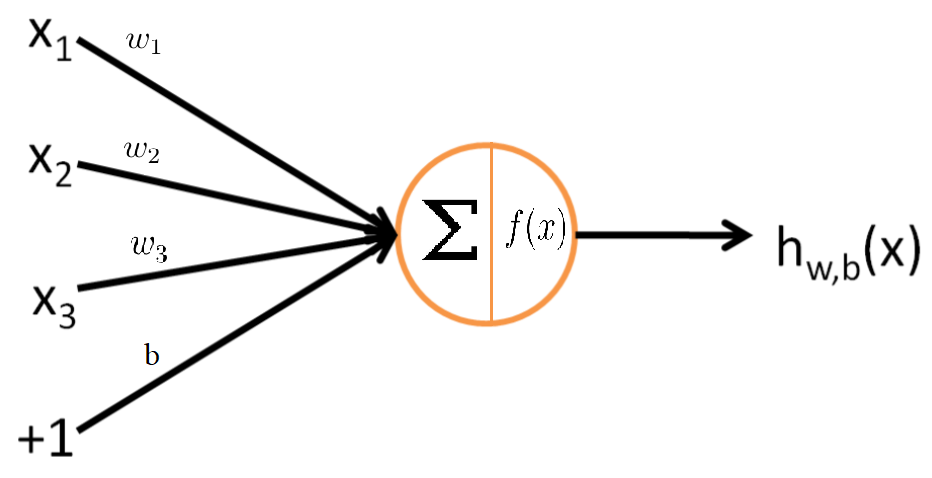
\includegraphics[width=0.5\linewidth]{abbildungen/perceptron.png}
  \caption{A perceptron: A perceptron contains a neuron and can take some inputs $\bm{x}$, applies weights $\bm{w}$ to them and generate an output $h_{w, b}(x)$. \cite{autoencoderSparse}}
\label{fig:perceptron}
\end{figure}

A perceptron is a neural network with only one neuron introduced by Frank Rosenblatt in \cite{perceptron}. The neuron in a perceptron has n inputs $x_1, x_2, ..., x_n$ which can be written as $\bm{x} = \left(x_1, x_2, x_3, \cdots, x_n \right)^T$ with an intercept input being +1, which is also called the bias term, the weights $w_1, w_2, ..., w_n$ applied to each input and an output $h_{w,b}(x)$ calculated by equation \eqref{eq:perceptronOut} with an activation function $f: \mathcal{R} \rightarrow \mathcal{R}$ indicating the behavior of the neuron. Examples for these functions are identity function \eqref{idFnc}, Heaviside function \eqref{heavisideFnc} and logistic function \eqref{logFnc}. The output behavior of the logistic function is shown in figure \ref{fig:logistic}. 
	\begin{equation} \label{eq:perceptronOut}
			h_{w,b}(x) = f(\bm{W^Tx}) = f(\overset{n}{\underset{i = 1}{\sum}}w_ix_i + b)
	\end{equation}
	\begin{equation} \label{idFnc}
			f(x) =  x
	\end{equation}
	\begin{equation} \label{heavisideFnc}
			f(x) =  H(x) = \left\{
		\begin{array}{ll} 
			0  & \mbox {, }x < 0 \\
			1 & \mbox {, }x  \leq 0
		\end{array}
	\right.
	\end{equation}
	\begin{equation} \label{logFnc}
			f(x) =  \frac{1}{1+e^{-x}}
	\end{equation}
	\begin{figure}[tbh]
  		\centering
    		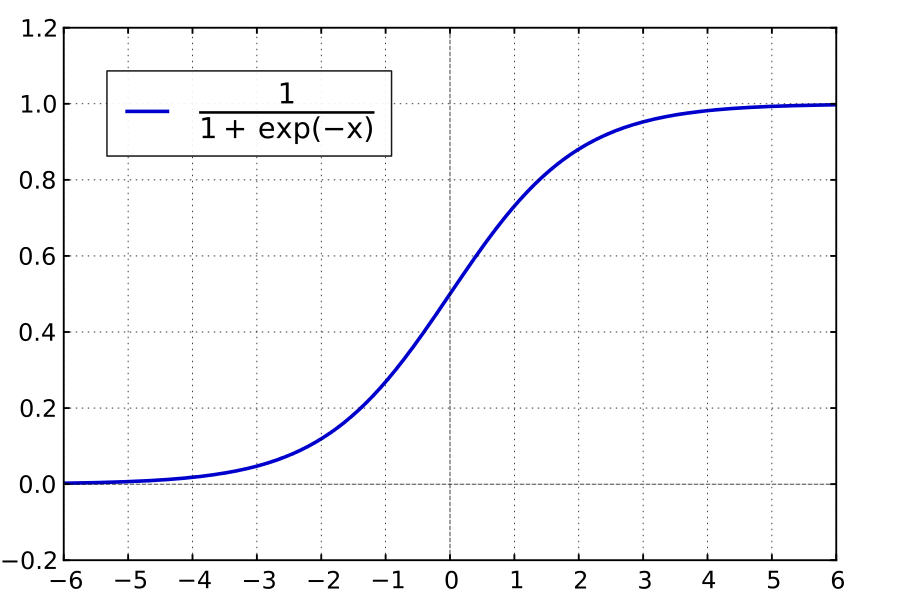
\includegraphics[width=0.8\linewidth]{abbildungen/logFnc.png}
  		\caption{Logistic Function: The value of the logistic function varies between 0 and 1 and can therefore represent the probability. The shape of the graph is also referred to as a Sigmoid curve.}  
		\label{fig:logistic}
		\end{figure}

The choice of the activation function must be made according to the task the network should handle. In case of a neuron with an all-or-nothing behavior, it is said to be active when the function value of $f$ exceeds a threshold, else it is inactive.

Since the effects of each inputs or each features on the output are controlled by the weights, the goal of training a neural network is to adjust the weights $w_i$ inside it so the output $h_{w, t}$ is as accurate as possible according to the task. For example, in a classification problem, the output of the well-trained network should correspond to the correct class of the objects it takes as an input. For this, choosing an activation function defining the output suitably for the task is crucial. In a linear regression problem where the output is linearly related to the input, a linear function might be more suitable and a function as step function that can be only 0 or 1 might be better for a binary classification with two competing classes. The higher the polynomial degree the activation function has, the finer the output can be tuned and accordingly, the more complex the task can be e.g. more possible classes the system can distinguish. On the other hand, if the chosen function is overly complex, it would cost more computing time than necessary for a simple task. 

The perceptron is only a neural network with only a single neuronal unit. The neural network commonly used in computer vision are consisted of many layers of neurons. To be able to understand the neural networks further, their learning processes should be understood. This includes how the knowledge is exchanged between each components and what is crucial to develop the right intelligence for the intended tasks. In the next section, the optimization of the networks with the common methods and possible mistakes are explained. 

%Network Optimization
\section{Network Optimization} \label{methods}
Before an ANN can perform the given task on its own, it must be trained first. By training an ANN, the weight of each neurons is adjusted so that it can generate the most accurate output for the desired prediction. As in figure \ref{fig:annSimp}, we will use the definitions from \cite{autoencoderSparse}, the output $\bm{a}_i^{l+1} = f(\bm{z}^{(l+1)})$ is the output from the activation function of the unit $i$ in layer $l+1$ computed from its input $\bm{z}^{(l+1)}$. Its weights $w_{ik}^{l+1}$ are assigned to its input $z^{l+1}_k$ and its bias term $b_i$. For the first layer $L_1$, the input layer, its input is $z^{(1)}_k = x_k$, the original inputs enter the first layer. For demonstration, the entering input $z^{(2)}$ and the forwarded output of the activation function of layer 2 with units $i \in \{1, 2, 3\}$ are:
	\begin{equation} \label{eq:act1L2} 
		a_1^{(2)} = f(w_{11}^{(1)}x_1 + w_{12}^{(1)}x_2 + w_{13}^{(1)}x_3 + b_1^{(1)})
	\end{equation} 
	\begin{equation} \label{eq:act2L2} 
		a_2^{(2)} = f(w_{21}^{(1)}x_1 + w_{22}^{(1)}x_2 + w_{23}^{(1)}x_3 + b_2^{(1)})
	\end{equation} 
	\begin{equation} \label{eq:act3L2} 
		a_3^{(2)} = f(w_{31}^{(1)}x_1 + w_{32}^{(1)}x_2 + w_{33}^{(1)}x_3 + b_3^{(1)})
	\end{equation} 

Then, these outputs from the second layer, the hidden layer, are assigned weights $w_{ik}^{2}$ and used to calculate the output of the final layer, the output layer $L_3$, which is also the output of this shallow neural network: 

	\begin{equation} \label{eq:output3ANN} 
		h_{w, b}(x) = a_1^{(3)} = f(w_{11}^{(2)}a_1 + w_{12}^{(2)}a_2 + w_{13}^{(2)}x_3 + b_1^{(2)})
	\end{equation} 

We can see that the outputs of each layer can be calculated consecutively from the former layers - from the beginning to the end only in the forward direction. A neural network with this behavior is also referred to as a feedforward neural network. Generally put, the outputs and inputs of the layers can be defined with following equations.
	\begin{equation} \label{eq:outputsANN} 
		\bm{z}^{(l+1)} = \bm{w}^{(l)}\bm{a}^{(l)} + \bm{b}^{(l)}
		\bm{a}^{(l+1)} = f(\bm{z}^{(l+1)})
	\end{equation} 

With this kind of networks, an effective strategy to adjust the weights according to the outputs is to trace the relations of the outputs from the outer layer back to the inputs and weights of the previous layers - to trace the outputs backwards into the hidden layers of the neural network. This method is also called the backpropagation algorithm \cite{backprop1986}. 

\begin{figure}[tbh]
  \centering
    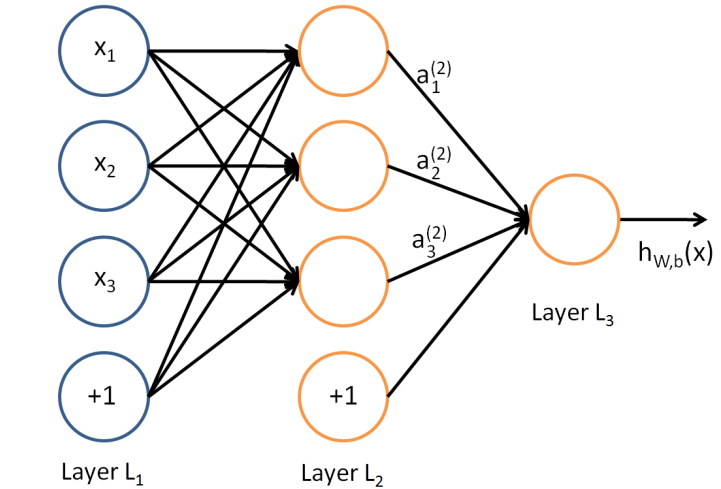
\includegraphics[width=0.5\linewidth]{abbildungen/annSimp.png}
  \caption{A simple ANN with a single hidden layer \cite{autoencoderSparse} An ANN takes the inputs through the neurons in the input layer $L_1$, then the weighted inputs are passed forward to the hidden layer $L_2$. The hidden layer then apply the activation function on the total inputs from the first layer and pass the calculated outputs $a_i^2$ to the output layer $L_3$. Finally, the output of the output layer $h_{w,b}$ is returned as the result.}
  \label{fig:annSimp}
\end{figure}

\subsection*{Backpropagation} \label{sec:backGD}
A simple ANN as shown  in figure \ref{fig:annSimp} might be sufficient for a simple problem. With more complex input data e.g. images or audio, a more complex network is needed to be able to learn the structure of the data sufficiently. As an ANN ‘learns’, it adjusts the weights of each neuron in its layers which can quickly sum up to millions of neurons. The goal of the adjustment is to find a combination of the weights that leads to the most accurate prediction of the data. With this kind of complexity, it is not wise to just blindly change the parameters until we get lucky and find the right ones. Therefore, the questions are how these million parameters can be adjusted efficiently and which direction of the adjustment is the right one.

The first question can be answered by the backpropagation algorithm. This algorithm is created to generalize the learning procedure of a perceptron, a single layer neural network, to multiple layer neural networks \cite{backpropagation} and became popular among researchers after the publication of \cite{backprop1986}. The main idea of backpropagation is to trace back into the hidden layers to adjust the weights of each layer accordingly so as to reduce the differences between the produced output and the desired ones. 

For simplicity, the derivation of this algorithm will not be explained in this thesis. The general theory of the backpropagation algorithm is explained extensively in \cite{backpropagation}.

Since our goal for a classification task is now to minimize the error of the prediction according to the labels of the data, the second question has to be brought back. To find the correct direction of the weight adjustment to achieve our goal, we can use gradient descent to ‘climb down the hill’ of the cost function until we reach the valley, the minimum point as illustrated in figure \ref{fig:GD}. In the next section, variations and functions of this algorithm will be described in details \cite{overviewGD}

\begin{figure}[tbh]
  \centering
    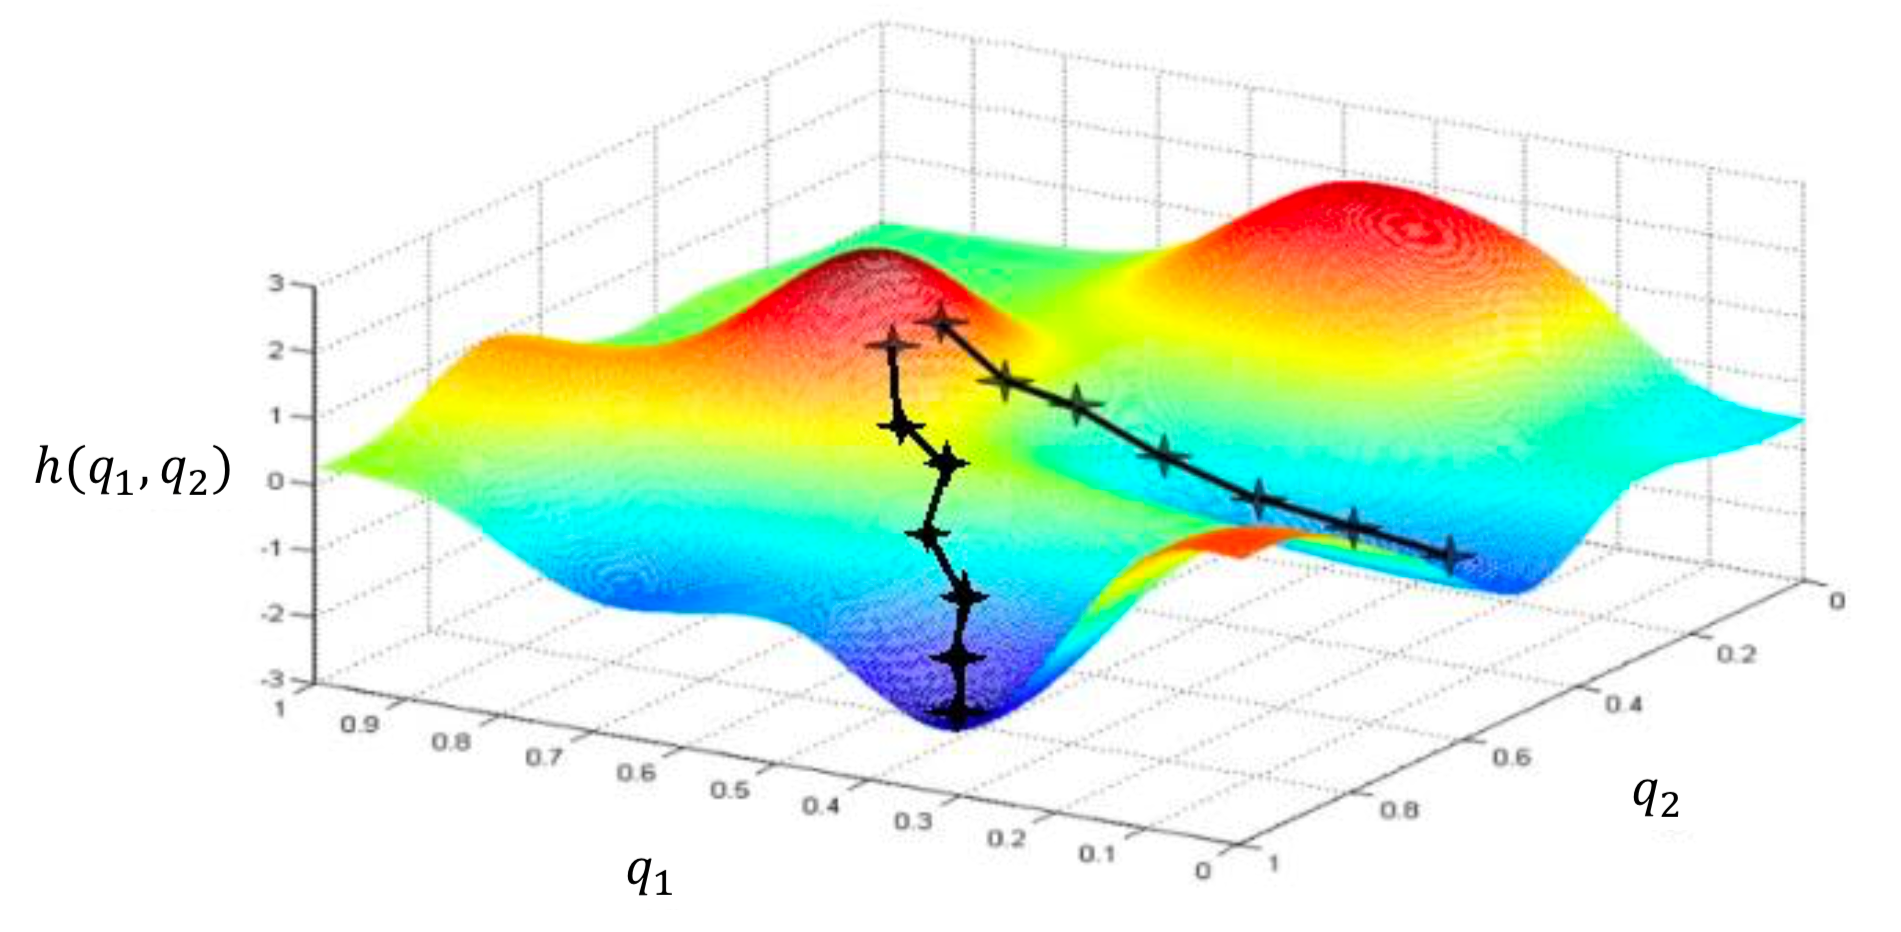
\includegraphics[width=\textwidth]{abbildungen/GD.png}
  \caption{Finding the minimum with gradient descent \cite{fig:GD}: With gradient descent, we try to minimize cost function $h(q_1, q_2)$ according to the parameters $q_1$ and $q_2$. As shown in the figure, it is also possible that we will find another local minimum if we chose another start point as the right start point takes us on the right route, the left point might take us on another route and to another local point. Therefore, initial parameters also influence the performance of the network.} 
  \label{fig:GD}
\end{figure}

\subsection*{Gradient Descent} \label{GD} 
The goal of training a neural network on a classification task is to find the parameter set with which it can make the most accurate prediction according to the input. In order to do this, we define a cost function of the network gets higher if the prediction is far from the reality, a function that measures the error of the network. Therefore, we can say that our goal is to minimize the value of the cost function - to find the parameter set that takes as to this point. The most effective way to do this is to always step in the direction that goes down the steepest. The steepness or the amount of change in a function over its parameters can be measured by its derivative $\frac{dJ}{d\theta_i}$ over its parameter $\theta_i$.  From the computed derivative, we know in which direction the strongest positive slope, the gradient, goes and make a step in the opposite direction - hence, gradient descent. The size of the step we take depends on the learning rate $\lambda$. Iteratively, we calculate the derivative and take a step until we reach the local minimum point of the cost function. 

An example of possible cost functions is the sum of squared errors $E_{sse}$ \eqref{eq:sseFnc} which sums up squared errors between a set of values. This can be used to measure how far off the $n$ predicted values $h_{w, b}(x_k)$ from the network are from the ground-truth values $y_k$.
	\begin{equation} \label{eq:sseFnc} 
		E_{sse} = \frac{1}{2}\overset{n}{\underset{i = 1}{\sum}}(h_{\bm{w},\bm{b}}(x_k) - y_k)^2
	\end{equation} 


The bigger the sum of the errors is, the more often and the bigger the differences were made. To make better predictions, the network should learn to reduce this sum - it should be optimized to minimize this error. According to equation \ref{eq:outputsANN}, the final output of the network $h_{w, b}(x_k)$ is a function of the weights $w_{ik}^{(l)}$ and the biases $b_i^l$. This means that the loss $E_{sse}$ is also parameterized by these values and adjusting them correctly can reduce the amount of error. The key to optimize the loss is to change the weights. Mathematically, a change of a function over a parameter is its derivative over the parameter. The change over a specific parameter, in particular, is represented by the partial derivative of this parameter. Gradient descent works by computing the change in the loss function caused by changes in the weights, i.e., the partial derivatives of the loss function over each weight $ \frac{\partial E_{sse}(\bm{w}, \bm{b})}{\partial w_{ik}^(l)}$ After the calculation, the weights and the biases are updated after \eqref{eq:weightUpdate} and \eqref{eq:biasUpdate}with the learning rate $\lambda$ controlling how big the adjustment after a round of backpropagation should be.

	\begin{equation} \label{eq:weightUpdate} 
		w_{ij}^{(l)} = w_{ij}^{(l)} - \lambda \frac{\partial}{\partial w_{ij}^{(l)}}E_{sse}(\bm{w}, \bm{b})
	\end{equation} 
	\begin{equation} \label{eq:biasUpdate} 
		b_{i}^{(l)} = b_{i}^{(l)} - \lambda \frac{\partial}{\partial b_{i}^{(l)}}E_{sse}(\bm{w}, \bm{b})
	\end{equation} 


The gradient descent algorithms need the input data to calculate the gradients. There are several variations of how much data we want to use for the calculations and which algorithms we use to calculate the gradient. First, the variation on the data amount will be introduced. This section is based on \cite{overviewGD}.

\subsubsection*{I Variations of Gradient Descent}
The amount of input data used for the calculation of the gradient has an impact on the accuracy of the computation. The more input data is used, the more accurate the value will be but also the longer the computation will take. By changing the amount of data, we can tweak the balance between the speed and the accuracy of the calculation. There are three common ways to do this: use the entire training dataset, use only one sample at a time, or take a sample batch from the dataset. 

\paragraph*{i) Batch Gradient Descent} Batch gradient descent uses the whole training dataset to calculate the gradients for each step. This makes it comparatively slow, memory-expensive and incompatible for updating gradient online with new examples coming in. However, since there is no fluctuation between the data for each calculation, it surely finds a minimum according to the initial parameters it started from, the global one for convex surfaces and a local minimum for non-convex surfaces. An example of these surfaces is visualized in figure \ref{fig:convex}. With this variation, we prioritize the accuracy more than time.  

\begin{figure}[tbh]
  \centering
    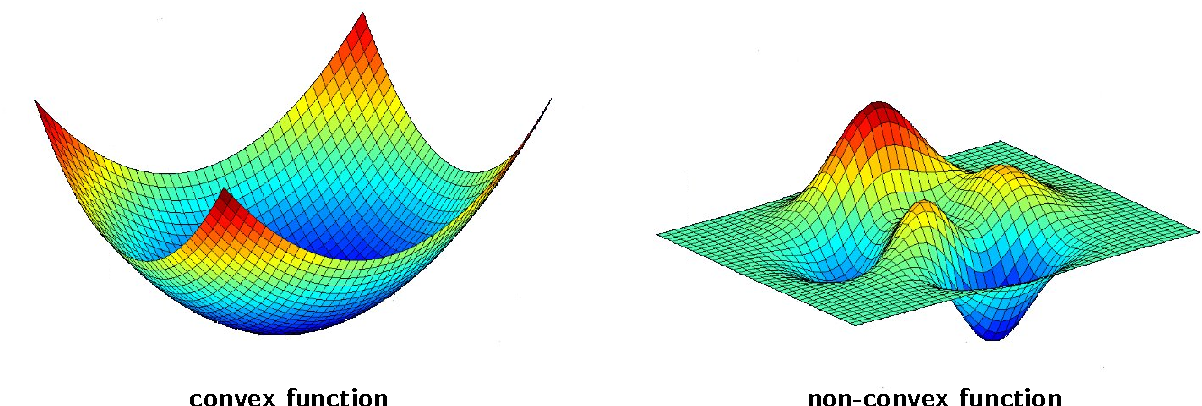
\includegraphics[width=0.8\textwidth]{abbildungen/convex.png}
  \caption{Convex and non-convex functions: A convex function has only a single minimum. A non-convex function, in contrary, has several local minima with a global minimum, the lowest minimum.} 
  \label{fig:convex}
\end{figure}

\paragraph*{ii) Stochastic Gradient Descent} \label{stochGD}This variation of gradient descent makes the opposite trade-off to the batch gradient descent by randomly taking just one training sample for each gradient calculation. Therefore, it takes much less time to calculate and update parameters which is more suitable for training online. Since there is variance between each step, the fluctuation can cause overshooting when converging to a minimum. While this can affect the path to the exact minimum, it also allows finding a better local minimum by springing out of the valley in which it started. Furthermore, there is a solution to the overshooting problem: a slowly decreasing learning rate has been shown to help SGD to convert to an exact minimum as the batch gradient descent \cite{overviewGD}. 

\paragraph*{iii) Mini-batch Gradient Descent} The small-batch gradient descent is the most popular variation of the gradient descent algorithm for training a neural network. It is practically in the middle of the former two variations as the gradient is calculated by using a batch of samples from the training dataset - not all of the dataset and not just a single sample. By doing this, there is less fluctuation between each parameter updates which means a more stable convergence. In the experiments in this thesis, this method is used with a batch size of 32 samples each iteration.

Apart from changing the amount of data used for the gradient calculation, we also can use an optimization method to counter different challenges in the process of finding the right parameters. Now, two examples of available optimization will be described.

\subsubsection*{II Optimization algorithms for Gradient Descent}
\paragraph*{i) Momentum} The momentum method \cite{momentum} is used to counter the problem of oscillating path caused by unevenly steep slopes in directions of different parameters. This is also found when the features significantly vary in their values. An illustration of such problem is shown in figure \ref{fig:ovalPlane}. This method adds a part of the past update vector to the recent one creating an acceleration along the way to the valley. The parameter is updated after equation \eqref{momentumFnc} and \eqref{momentumthetaFnc}.

	\begin{equation} \label{momentumFnc}
			v_t = \gamma v_{t-1} + {\eta}{\bigtriangledown_\theta}E(\theta)
	\end{equation}

	\begin{equation} \label{momentumthetaFnc}
			\theta = \theta - v_t
	\end{equation}

with an update vector $v_t$ at step $t$, a cost function $E$ and the parameter that should be update $\theta$.

This original momentum algorithm uses the recent position of the parameters to perform the update of the parameter. Therefore, it has no insight of the next step and could make a sub-optimal adjustment. Next, an algorithm is introduced that uses the information from the future position of the parameters.
 
\begin{figure}[tbh]
  \centering
    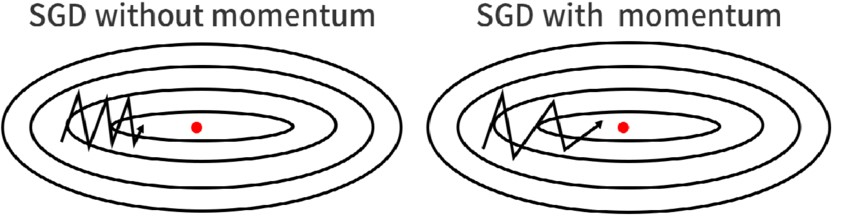
\includegraphics[width=\textwidth]{abbildungen/momentumGD.jpg}
  \caption{Stochastic Gradient Descent with and without momentum \cite{fig:momentumGD}: Without the momentum optimization, the path of the gradient descent suffers from the oscillation when the features are of different multitudes as can be seen in the left picture. The momentum accumulated in the direction of the longer axis allows for a more direct descending path as depicted on the right.} 
  \label{fig:ovalPlane}
\end{figure}

\paragraph*{ii) Nescerov Accelerated Gradient (NAG) \cite{NAG}} This algorithm is the speed-up version of the momentum. Instead of using the present parameter position to calculate the gradient, it approximately calculates the gradient of the slope in the next step. This way, it adapts to the next position and looks ahead down the hill instead of just adjusting itself to the hill as it descends. According to equation \eqref{eq:nescerovFnc}, this algorithm calculates the gradient using $\theta - \gamma v_{t-1}$, the approximated of the future $\theta$, instead of just $\theta$, to calculate the vector. Then, it similarly updates the parameter using the calculated vector \eqref{eq:thetanescerovFnc}.

	\begin{equation} \label{eq:nescerovFnc}
			v_t = \gamma v_{t-1} + {\eta}{\bigtriangledown_\theta}E(\theta - \gamma v_{t-1}) 
	\end{equation}
	\begin{equation} \label{eq:thetanescerovFnc}
			\theta = \theta - v_t
	\end{equation}

\paragraph*{iv) Adaptive Moment Estimation (Adam)} Adam \cite{adam} is an adaptive learning method, i.e. it computes learning rates for each parameter individually. With an adaptive method like this, the size of the update for a parameter is smaller, the more frequent this parameter is updated. As its name implies, Adam also uses moments to calculate the updates as following: first, it calculates and collects the decaying moment according to equation \eqref{eq:AdammomentFnc} with the decay rates $\beta_1$ and $\beta_2$. Then, it corrects their bias towards 0 caused by initialized values $m_v$ and $t_v$ being 0, according to \eqref{eq:AdamcorrectFnc}. 

	\begin{equation} \label{eq:AdammomentFnc}
		\begin{split}
			g_t = & {\bigtriangledown_{\theta_t}}J(\theta_t) \\
			m_t = \beta_1m_{t - 1} &+ (1 - \beta_1)g_t \\
			v_t = \beta_2v_{t - 1} &+ (1 - \beta_2)g^2_t
			\end{split}
	\end{equation}

	\begin{equation} \label{eq:AdamcorrectFnc}
	\begin{split}
		\hat{m}_t = \frac{m_t}{1 - \beta_1^t} \\
		\hat{v}_t = \frac{v_t}{1 - \beta_2^t}
	\end{split}
	\end{equation}

Finally the parameters are updated with help of the calculated moments as defined in equation \eqref{eq:AdamupdateFnc}

	\begin{equation} \label{eq:AdamupdateFnc}
			\theta_{t+1} = \theta_t - \frac{\eta}{\sqrt{\hat{v}_t} + \epsilon} \hat{m}_t 
	\end{equation}

\paragraph*{Nesterov-accelerated Adaptive Moment Estimation (Nadam)} As the name implies, this algorithm is the combination of the previous two methods, the Nescerov accelerated gradient and Adam. This gives us the new parameter updating rule \eqref{eq:nadamupdateFnc} 
	\begin{equation} \label{eq:nadamupdateFnc}
			\theta_{t+1} = \theta_t - \frac{\eta}{\sqrt{\hat{v}_t} + \epsilon} \left( \beta_1\hat{m}_t + \frac{(1 - \beta_1)g_t}{1 - \beta_1^t} \right)
	\end{equation}
With this method, the gradient descent is accelerated and adapts well to both the curve of the cost function and different parameters at the same time.

After we addressed the method of training the network effectively using backpropagation and gradient descent. We will now introduce of the common perils in the training that can affect the performance of the network.

\subsection{Overfitting and Underfitting}
When training a neural network, choosing the right method to the problem and the given data is important to ensure that the network will learn the information necessary for the task. Then, choosing the right parameters so that the training goes as plan is also crucial. All these correct setups could only be optimal if we know what danger still awaits in the training which can compromise the performance of the model. The common problems occuring in the training are overfitting and underfitting. Overfitting is when the network adapts itself too much to the data and underfitting is when the network could not or would not adapt enough to learn the problem. More details and prevention methods to these problems are discussed now in this section. 
 
\subsection*{A. Overfitting}
Overfitting describes a situation when a model starts to learn unnecessary noises and irregularities in the training set and not the more relevant knowledge it should for the task. In the end, the network would not generalize well on new data because it has adapted itself too much on the training dataset. Similar to a student memorizing the answers to the exercise sheets but has no real knowledge about the underlying theories in the subject, the network will know the training data very well but will not perform well on the unknown data, the real test. The problem of overfitting is visualized in figure \ref{fig:underoverfitting} along with underfitting. The overfitted curve adjusts itself to each and every data point it has seen in the training. Consequently, it has overall an inaccurate representation of the true distribution even if the error calculated on the given training data is very low. Since the main goal of training the networks is not only to learn specifically about the training data, but to have enough general knowledge to perform the task on the unknown data, overfitting can compromise the performance of the trained networks.

Overfitting can happen especially when the model is complex enough and is trained repeatedly too much on the same data, e.g. too many epochs have passed or too little data for the complexity of the networks. We should suspect a problem of overfitting when the model has a good performance or a very low loss value in the training data but has a low performance on other data. Note that this symptoms might also come from other underlying causes. 

\paragraph*{Prevention of Overfitting}
To prevent overfitting, we have to avoid over-training the models i.e. training further even if the model has reached the convergence of the loss function. Even an experience researcher cannot be certain of the point at which the training should be terminated. Therefore, more exact ways to automatically achieve this was developed. Here, two examples of such possibilities are listed: early stopping and training with weight decay.  

\subparagraph*{i. Early stopping} Ideally, we should stop training early enough so that the model has already learned to fit its function to the nature of the data seen in the training but not enough to overly fit it exclusively to this data. To know when to stop needs much experience and can also cost an unnecessary performance drop if not done right, therefore using an algorithm to automatically stop the training is introduced. For this, the training set is divided into an actual training set and a validation set with a proportion of 2 to 1 \cite{overfitearlystop}, then to observe the loss on the validation set after training e.g. for an epoch. An example for a stop criterion: if the validation loss increase relatively high after an epoch, the training is then stopped. Formally, after epoch $t$, we have the validation loss $E_{va}(t)$ defined by a loss function for training and the lowest validation error so far in the training $E_{opt}(t) = \underset{t'\leq t}{min}E_{va}(t')$. We can define the generalization loss $GL(t)$ as the relative increase of the validation error over the recorded minimum as in \eqref{eq:earlystop}. If the generalization loss exceeds a threshold, the training should stop. 
	\begin{equation} \label{eq:earlystop}
			GL(t) = 100 \left( \frac{E_{va}(t)}{E_{opt}(t)} - 1 \right)
	\end{equation}
This algorithm stops training automatically when the risk of overfitting appears at a cost of extra training time. \cite{overfitearlystop} shows different setup and the tradeoff between time and performance increase. 
\subparagraph*{ii. Weigth Decay} Another possibility to prevent overfitting is to penalize big weights in the network. As we saw in $\ref{perceptron}$, each neuron has its weights to adjust the influence of the input on the output. With weight decay, the original loss function $E_0(\bm{w})$ is combined with the weight penalizing term into a new cost function as follow: 	
	\begin{equation} \label{eq:weightdecay}
			E(\bm{w}) = E_0(\bm{w}) + \frac{1}{2}\lambda\underset{i}{\sum}\bm{w}_i^2
	\end{equation}
where $\lambda$ is the learning rate and $\bm{w}$ the weights of the neurons. 

By penalizing the weights, we put constraints on the network and limit its freedom to adjust the parameters freely. This prevents the weights from growing unnecessary large and was proved to improve the generalization of the network \cite{overfitweightdecay}. It is also a preferable alternative to eliminating the number of weight to keep the network as simple as possible as proposed in \cite{overfitweightelim}.

\subsection*{B. Underfitting}
The problem of underfitting is the opposite of the overfitting case \cite{underoverfitting}. It happens when the network is not complex enough to learn the underlying nature of the problem. For example, if we want to find a fit for non-linearly distributed data a linear model, the model cannot be adjusted enough to describe the problem accurately. To avoid this, the choosing a network with proper complexity to the problem is crucial. The choice must also take into account the amount of data we have to also avoid overfitting at the same time. 

\begin{figure}[tbh]
  \centering
    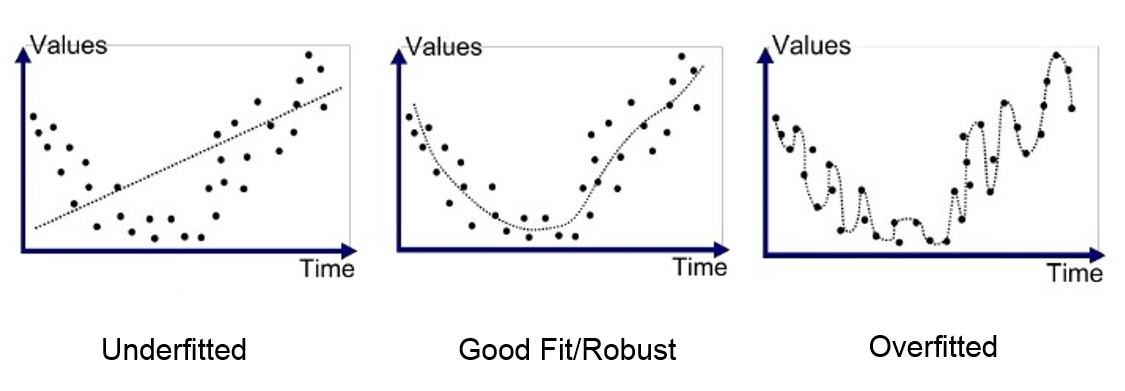
\includegraphics[width=\textwidth]{abbildungen/overunderfitting.png}
  \caption{Overfitting and Underfitting: A good representation of the underlying distribution of the given data points is depicted in the middle. The underfitted representation has insufficient dimensionality to represent the real distribution as shown in the left graph. If the network has overfitted itself, as on the right, it tries to adjust itself to every given point and thus would mostly make poor predictions on unknown data points.} 
  \label{fig:underoverfitting}
\end{figure}

As the neural network becomes more complicated with more neurons and more layers, the relation between the output, the weights and the inputs become more complex and can handle more difficult tasks effectively as a perceptron cannot. To handle such inputs as images or audio files, a network of higher complexity is necessary for effective task handling. In computer vision, one type of neural networks in particular has become very popular and is also included in the Domain Separation Network we use here. Therefore, the structure of this neural network, the Convolutional Neural Network, will be explained more in detail in section \ref{cnn}.


%CNN
\subsection{Convolutional Neural Network} \label{cnn}
The goal of computer vision is to make machines see as we can with our eyes and brains. Intuitively, we identify object with noticeable high-level features such as body composition of an animal or part of an object. For a machine to be able to do this, it requires building up detectable low-level features together until they represent a part. Dots build up lines, lines join to create edges and edges define forms of a part of an object that hints to an object. A CNN is built of many stages extracting different features on different levels to put them back together and make prediction about the image as a whole.  Each stage consists of layers of neurons which are described further in this section. The definition of the structure is based on \cite{convVision}.

\paragraph*{Common Layers of the Convolutional Neural Networks}
\subparagraph*{i. Filter Bank Layer or Convolutional Layer} In this layer, different features in an input image are detected by different filters. Each filter has weights with a filter-specific kernel to 
convolve with the feature maps as described in Equation \ref{fig:conv} and each neuron has its receptive field or an area of image it scans for the feature. Because all areas of the images get scanned with the filters thoroughly, the features are detected even if their position changes. This process is visualized in figure \ref{fig:conv} Mathematically described, the 3D input array consists of $n$ 2D images $x_i$. The filter kernel $k_{ij}$maps the input $x_i$ to the feature map $y_j$ as an output according to equation \eqref{convFnc} where $\ast$ is the 2D discrete convolution operator defined as \eqref{convOpFnc}
\begin{equation} \label{convFnc}
			y_i = b_j + {\sum_i}k_{ij} \ast x_i
\end{equation} 
\begin{equation} \label{convOpFnc}
			h \ast x = \overset{\infty}{\underset{k_1 = -\infty}{\sum}}\overset{\infty}{\underset{k_2 = -\infty}{\sum}} \cdots \overset{\infty}{\underset{k_M = -\infty}{\sum}} h(k_1, k_2, \cdots, k_M) x(n_1 - k_1, n_2 - k_2, \cdots, n_M - k_M)
\end{equation}

The size of the output of the $n$-th layer $(M_1^n, M_2^n)$ will depend on the size of the input, the output from the $(n-1)$-th layer, $(M_1^{n-1}, M_2^{n-1})$ and the size of the kernel $(K_1^n, K_2^n)$ with a stride of size $(S_1^n, S_2^n)$ as follow \cite{flexHighCNN}:
\begin{equation}
			M_1^n = \frac{\left(M_1^{n-1} - K_1^n\right)}{S_1^n + 1} + 1 
\end{equation}
\begin{equation}
			M_2^n = \frac{\left(M_2^{n-1} - K_2^n\right)}{S_2^n + 1} + 1 
\end{equation}

As we can see from figure \ref{fig:conv} and the equations above, the feature map will be smaller after the convolution. To control the size change, padding can be used to extend the input around the edges. A typical padding variation is to extend the edges with zeros. The size of the output of the $n$-th layer $(M_1^n, M_2^n)$ will depend on the size of the input, the output from the $(n-1)$-th layer, $(M_1^{n-1}, M_2^{n-1})$ and the size of the kernel $(K_1^n, K_2^n)$ with a stride of size $(S_1^n, S_2^n)$ and $p$ zero padding size as follow \cite{convArith}:
\begin{equation}
			M_1^n = \frac{\left(M_1^{n-1} - K_1^n + 2p\right)}{S_1^n} + 1 
\end{equation}
\begin{equation}
			M_2^n = \frac{\left(M_2^{n-1} - K_2^n  + 2p\right)}{S_2^n + 1} + 1 
\end{equation}


\begin{figure}[tbh]
  \centering
    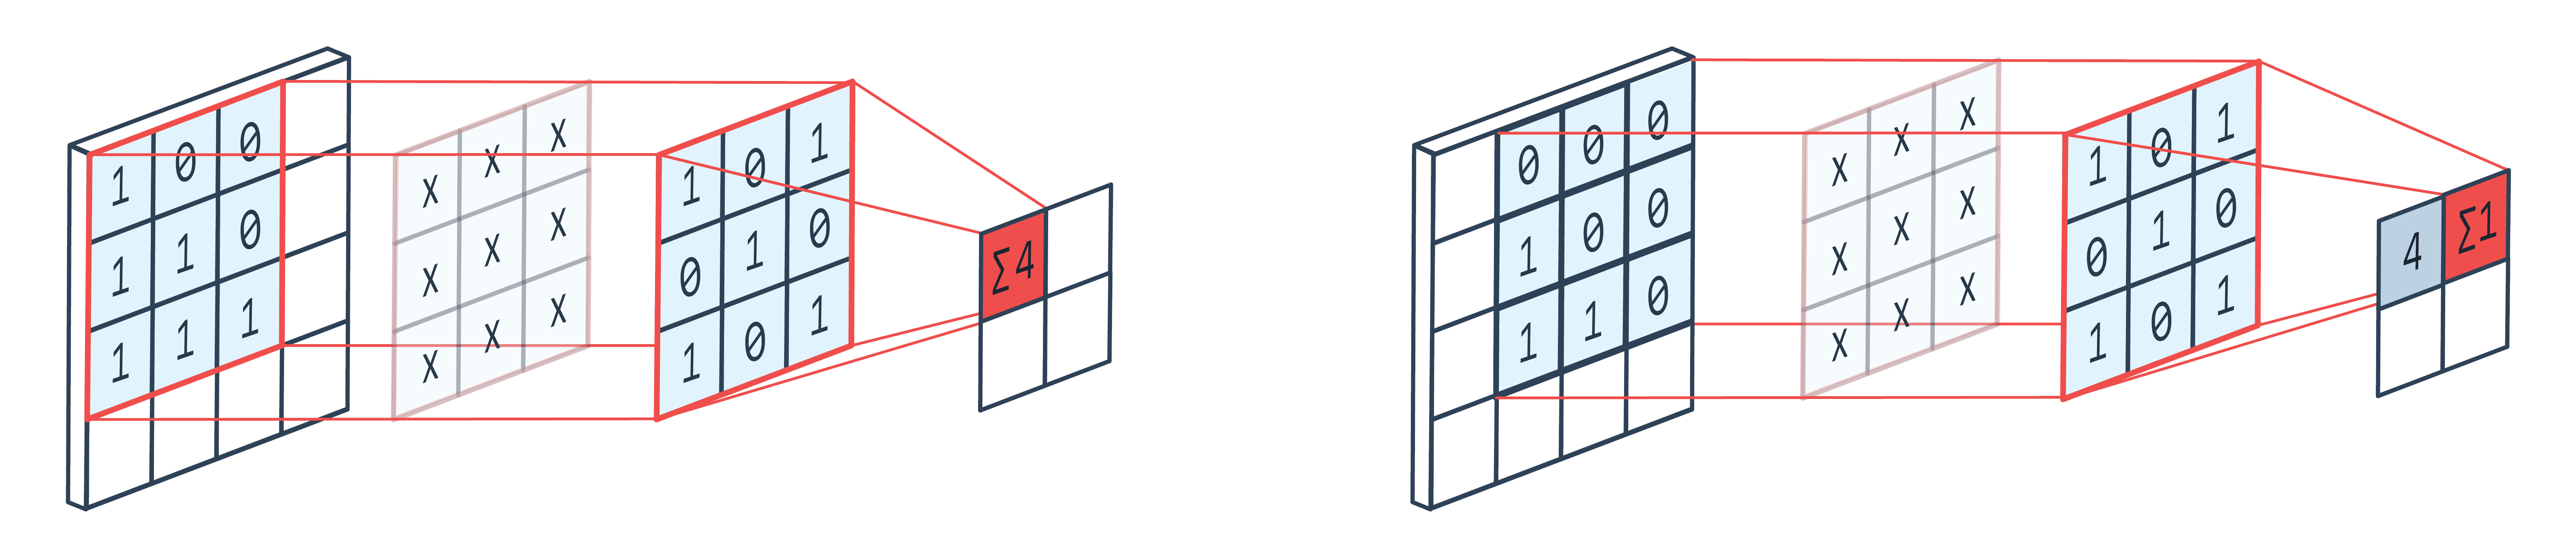
\includegraphics[width=\linewidth]{abbildungen/conv.png}
  \caption{Convolution with a 3x3 kernel \cite{fig:conv}: An 4x4 image is convolved with a 3x3 kernel. The kernel strides one pixel at a time and compute in each step a value for the output matrix. Since there is no padding, the dimension of the output is smaller than that of the input.} 
  \label{fig:conv} 
\end{figure}

\subparagraph*{ii. Non-linearity Layer}This layer hosts a nonlinear function used to compute the outputs of the neurons such as tanh function defined by equation \eqref{tanhFnc} or logistic function as defined in \eqref{logFnc}. In the method we use in this thesis, the rectified linear unit \cite{reluICML} defined by equation \eqref{reluFnc} is used which allows faster training than the $tanh$ function \cite{imgNet}. 
	\begin{equation} \label{tanhFnc}
			f(x) = \frac{e^x - e^{-x}}{e^x + e^{-x}}
	\end{equation}
	\begin{equation} \label{reluFnc}
			f(x) =  max(0, x)
	\end{equation}

\subparagraph*{iii. Pooling Layer:}This layer reduces the resolution of its input, the output of the previous layer, by computing a representative value such as the average value, using average pooling or the maximum value of a region in the input. Different outputs from these two methods can be seen in figure \ref{fig:pooling}. \cite{cnnpooling} has proved that using maximum value can achieve better performance. In the architecture we use, DSN also uses a model with max-pooling layers which samples out the maximum value to downsize the input and also makes its position invariant over bigger region \cite{flexHighCNN}.

\begin{figure}[tbh]
  \centering
    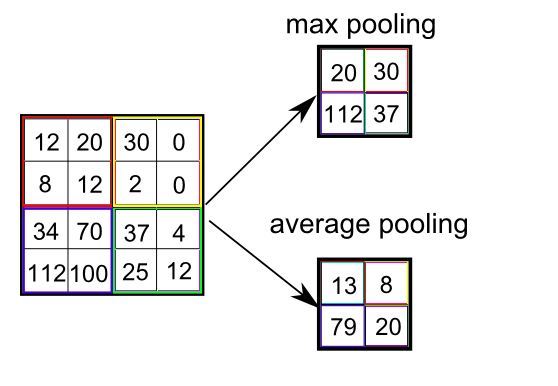
\includegraphics[width=0.6\linewidth]{abbildungen/pooling.png}
  \caption{Output of Max Pooling and Average Pooling \cite{fig:pooling}: From the same input matrix of dimension 4x4, a 2x2 pooling operation with a stride of 2 pixels gives an 2x2 matrix as an output with different value dependent from the method. The max pooling method pulls out the maximum value in each areas and the average pooling method calculates the average of the area. } 
  \label{fig:pooling} 
\end{figure}

A typical CNN contains two or three stages with these layers. Then, the outputs of various feature filters in the last stage are connected in the fully connected layer to compute final output in the desired form. For this purpose, it might get flattened into a one-dimensional vector. In our classification task, the probabilities of each classes are computed to be the final output. After all the stages, we get the output from the final output layer. An Example of a CNN with these layers are shown in figure \ref{fig:cnn}

\begin{figure}[tbh]
  \centering
    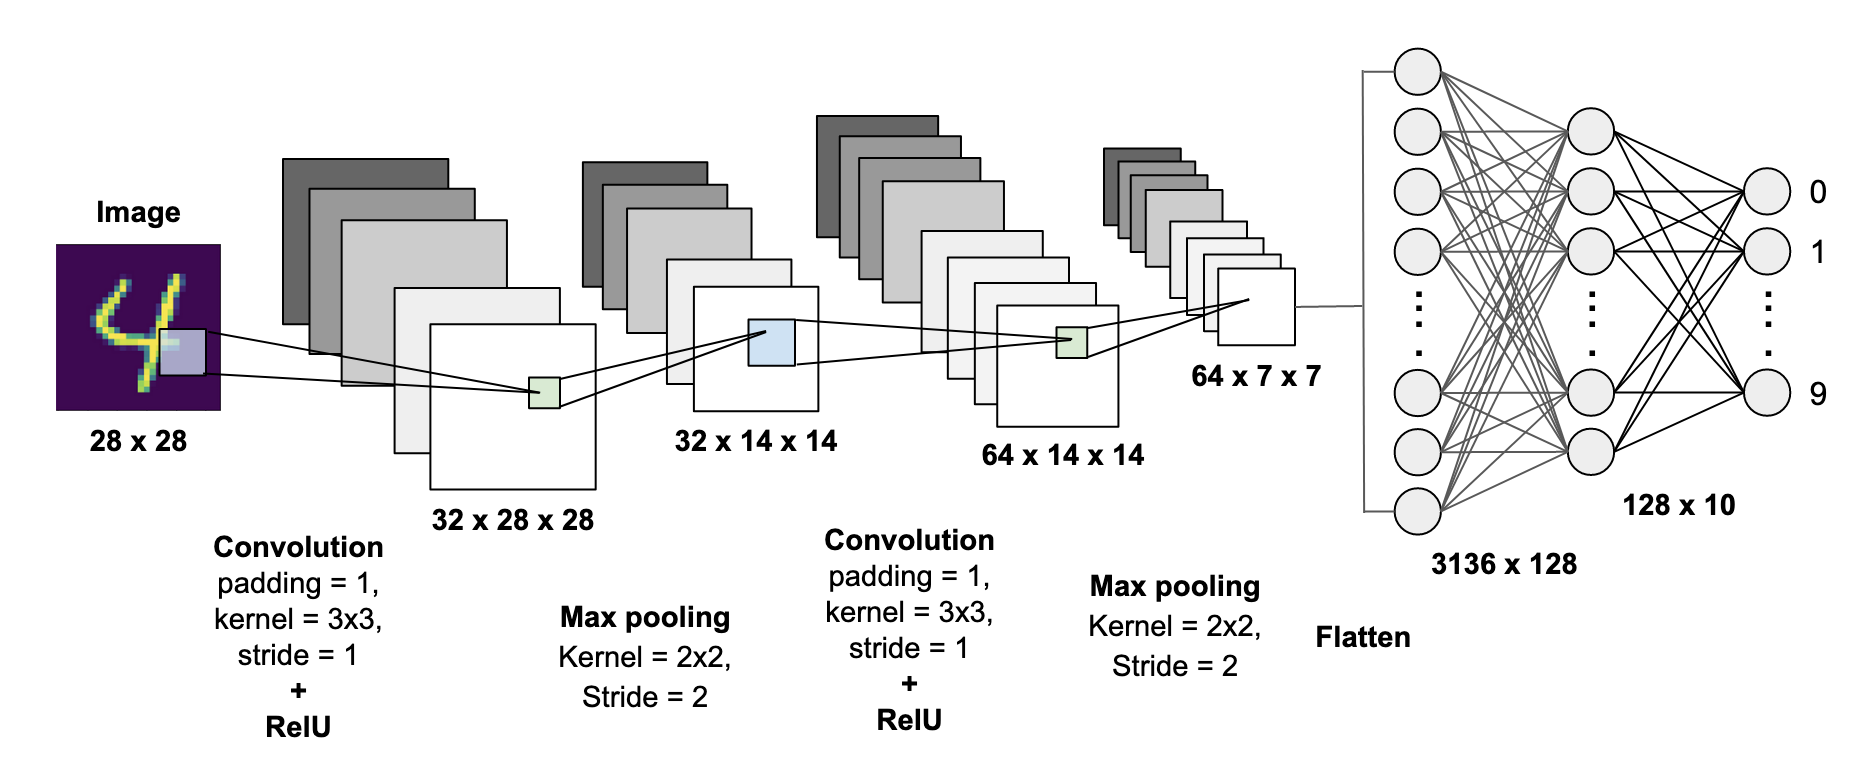
\includegraphics[width=\linewidth]{abbildungen/cnn.png}
  \caption{Convolutional Neural Network \cite{fig:cnn}: This CNN should recognize the number in the input image. It contains two stages with three layers: a convolutional layer, a non-linearity layer with ReLU, and a pooling layer. At the end, it should output the predictions on the class of the image being 0 to 9.} 
  \label{fig:cnn} 
\end{figure}

\paragraph*{Applications of the Convolutional Neural Networks}
The power of the deep convolutional neural networks are demonstrated in \cite{imgNet} as a team won the ImageNet Large Scale Visual Recognition Challenge 2012 \cite{ILSVRC2012} in both the classification and localization tasks with this kind of neural networks. Their deep CNN has 60 million parameters and 650,000 neurons with five convolutional layers followed partly by max-pooling layers and three fully connected layers. A way to effectively train this large network is through stochastic gradient descent method described in Section \ref{stochGD}.

Furthermore, the CNN was used, for example, to extract and transfer style of images in \cite{convImgStyle}. Through several convolutional layers, the features of the image styles are extracted and can be used to combine with another image to represent that image in the extracted style (see figure \ref{fig:styleTrans}). In this work, we can also see the different levels of extracted features from different layers in the CNN as shown in figure \ref{fig:cnnLevel}

\begin{figure}[tbh]
  \centering
    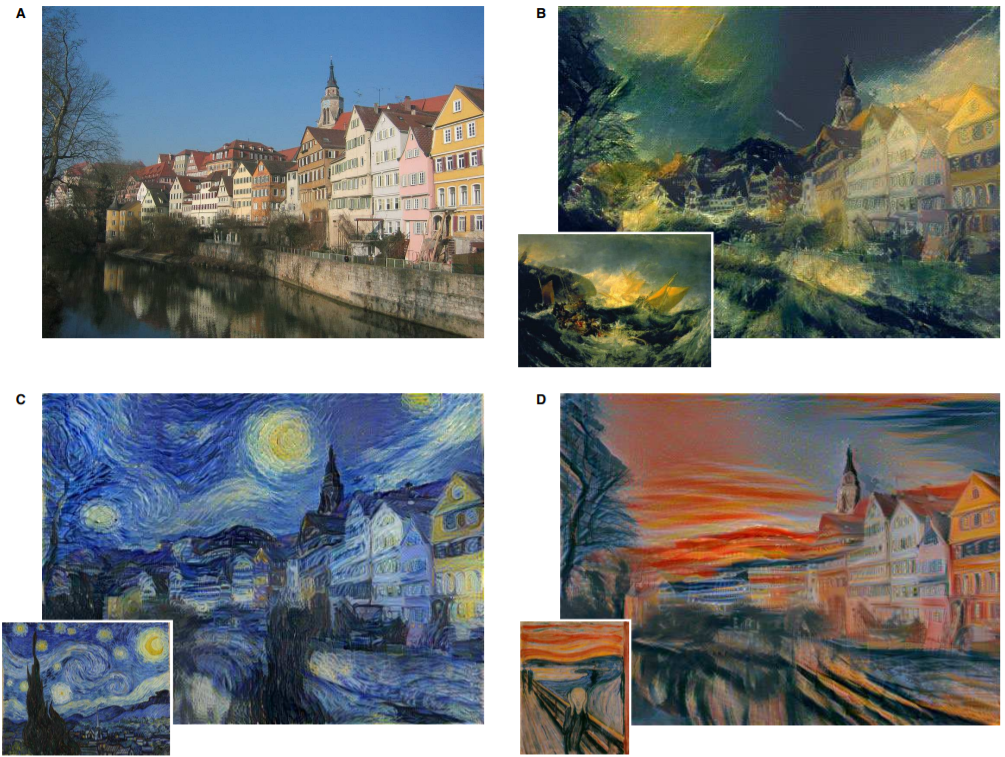
\includegraphics[width=\linewidth]{abbildungen/styleTrans.png}
  \caption{Style Transfer by a CNN: By extracting the style of famous pictures and the contents of the image, a CNN can produce the given image in the given styles \cite{convImgStyle}.} 
  \label{fig:styleTrans} 
\end{figure}

\begin{figure}[tbh]
  \centering
    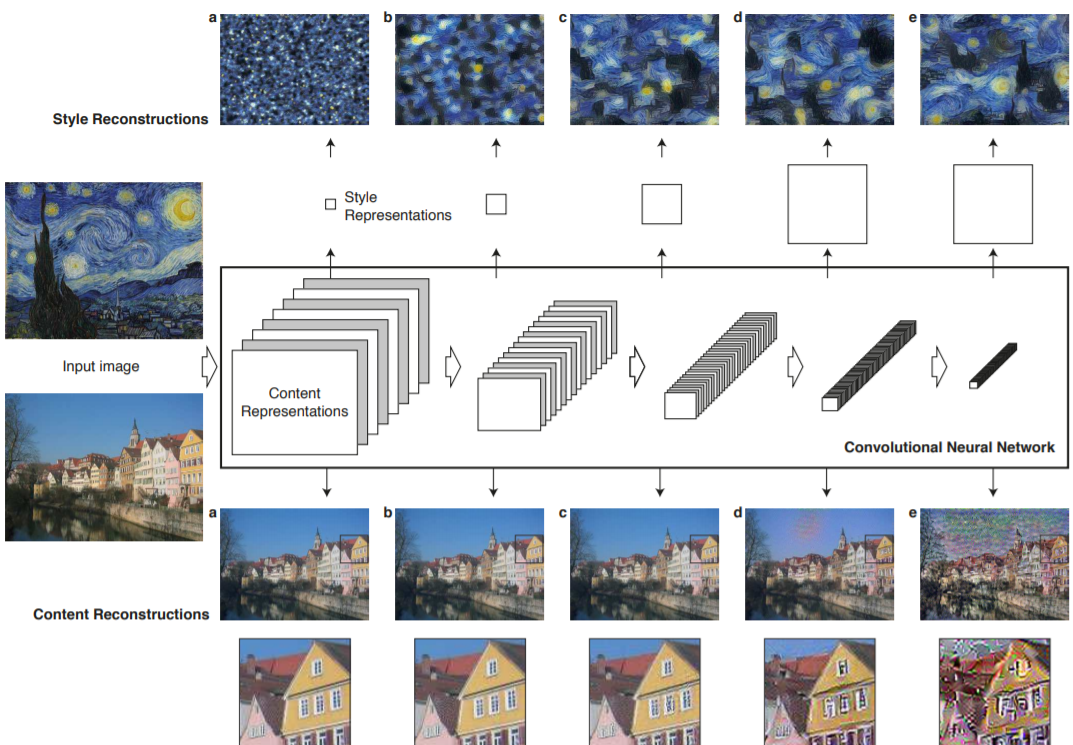
\includegraphics[width=\linewidth]{abbildungen/cnnLevel.png}
  \caption{Output from different levels in a CNN: Deeper levels of a CNN can capture more high-level details of the style and the components of the images whereas the first levels acquire the details finer on the pixel level.} 
  \label{fig:cnnLevel} 
\end{figure}


%Autoencoders
\subsection{Autoencoders} \label{sec:autoencoders}
When working with images, the common challenges are dealing with the dimensions of the image. The motivation for the autoencoders is to find lower-dimensional representations of a high-dimensional input from which the original input can be reconstructed. For example, images with higher solution can be represented by lower-dimensional features with the autoencoders. Furthermore, to be able to represent something with less details, its significant points must be preserved. This way, the autoencoders can also extract features and create representations that are more suitable for further tasks \cite{autoencoderVisualize}. 

\begin{figure}[tbh]
  \centering
    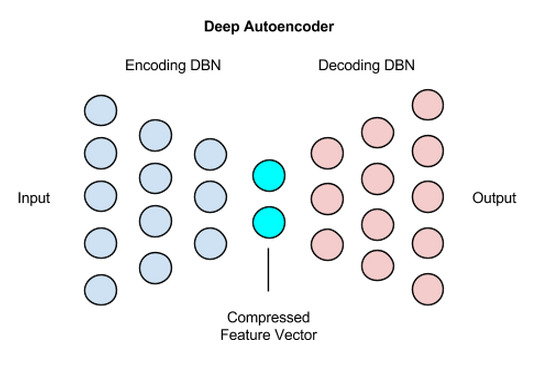
\includegraphics[width=0.6\linewidth]{abbildungen/autoencoders.png}
  \caption{Example of an autoencoder: The autoencoder encodes an input into a lower-dimensional feature vector. This representation can then be decoded back to higher-dimensional inputs as the original \cite{fig:autoencoders}.}
  \label{fig:autoencoders} 
\end{figure}

An autoencoder, therefore, has two essential parts: an encoder and a decoder. The encoder extracts the significant features of the input and maps these into a lower-dimensional output. The decoder then maps the encoded output, ideally, back to the original information. Formally, the encoder has a function that maps a $d$-dimensional input $x_i \in \bm{X}$ with a function $f$ a representation $\bm{h} = f(\bm{x}), h \in \bm{H}$ with dimension $p \ll d$. Note that it is possible to have an autoencoder with $p = p_1 + p_2 > d$ \cite{autoencoderDeep} which is not relevant in our case. Then, the decoder has a function $g$ that maps back the representation $h$ to a $d$-dimensional output. The mapping functions work in a way that:
 	\begin{equation} \label{eq:autoencoder}
			|x - (g \circ f)(x)| \rightarrow min
	\end{equation}

The representation the decoder maps from the encoded values $(g \circ f)(x)$ should be as similar to the original input $x$ as possible - the difference to the original input must be minimized. By trying to find lower-dimensional representations of the inputs and to decode these representations back to outputs resembling the original ones, the autoencoders find applications in many fields as feature extracting and dimension reduction are generally helpful to the working of neural networks. In the DSN, the autoencoders also extract representations used to apply domain adaptation and to train the classifier. 



\paragraph*{Applications of the Autoencoders} 
\subparagraph*{Dimensionality Reduction \cite{autoencoderVisualize}} The main benefit of the autoencoders is that they can find representations of the inputs with lower dimensions than the original input. An autoencoder can find codes for the images with 28x28 pixels from the MNIST dataset with only two dimensions that still show a clear separations of classes as visualized in figure \ref{fig:mnistvisualize}, even better than those created by the principle component analysis (PCA) \cite{PCA}, a method popularly used to extract features. The autoencoder can find representation for pictures of human faces with only 30 dimensions as shown by \cite{autoencoderFace}.

\begin{figure}[tbh]
  \centering
    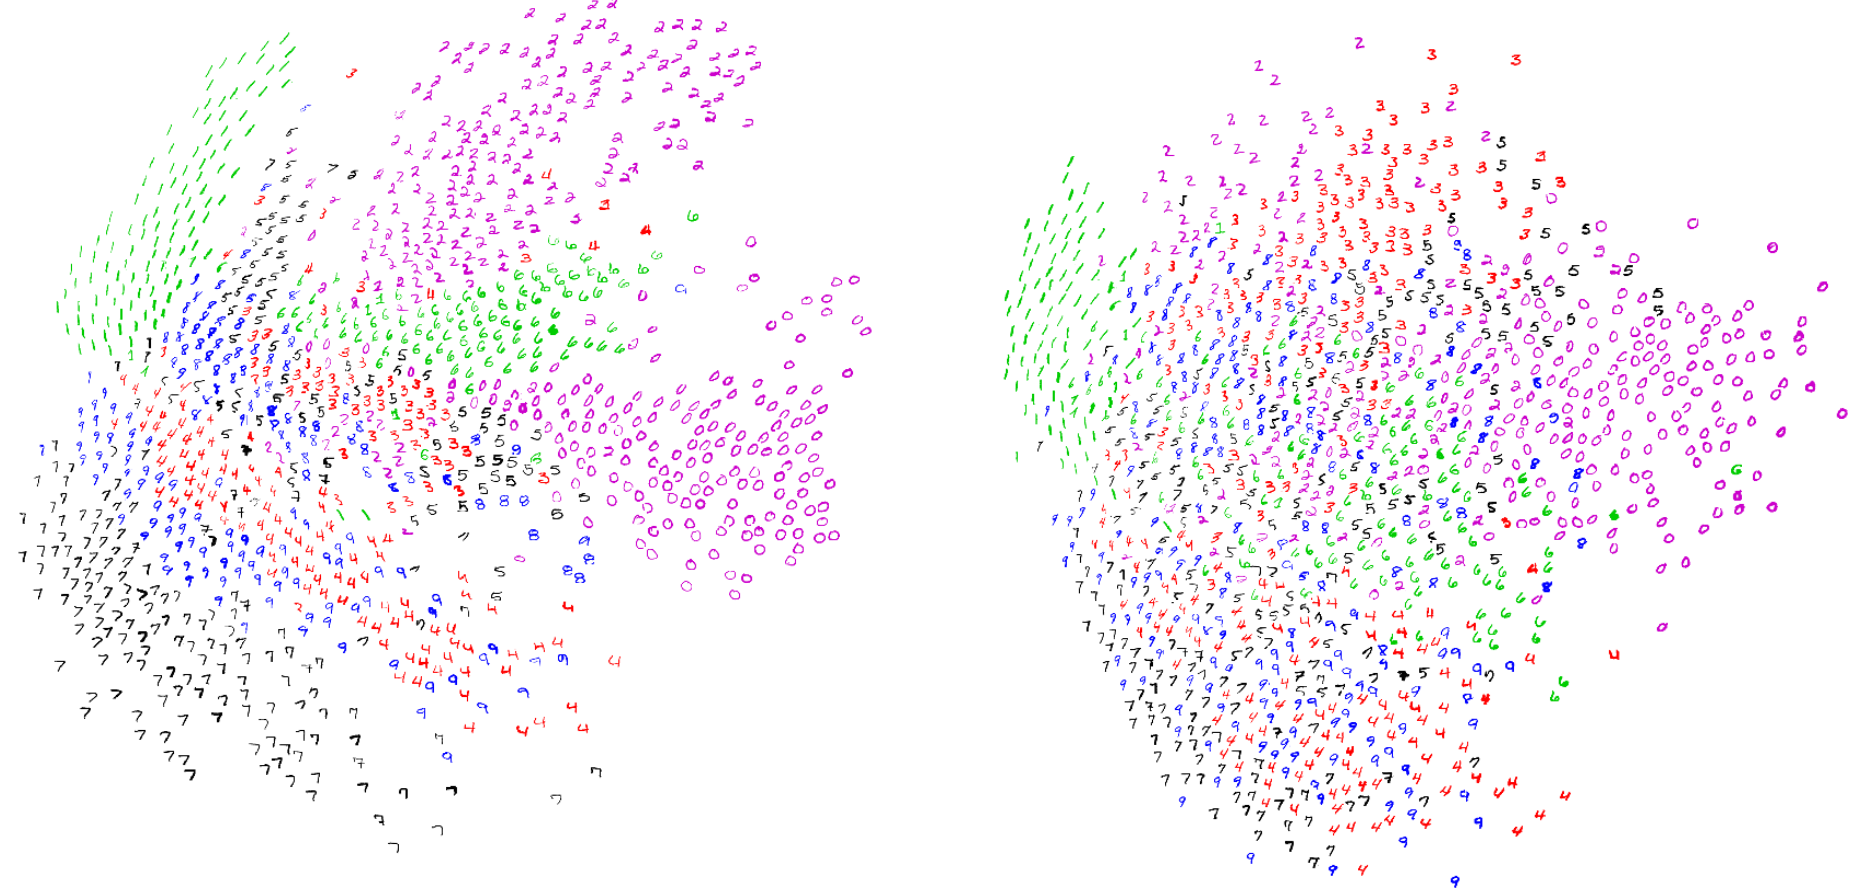
\includegraphics[width=\linewidth]{abbildungen/mnistvisualize.png}
  \caption{Visualizations of encoded two-dimensional Vector from the MNIST dataset: The encoded vectors created by an autoencoder (left) show better separated groups of each classes than those created by using principle component analysis method (right).}
  \label{fig:mnistvisualize} 
\end{figure}

\subparagraph*{Extracting Features}
Being able to compress data into lower-dimensional, the autoencoders know how to find the essential features of the data. By using features discovered by the autoencoders, the results of the classifier has been improved as shown by \cite{autoencoderDenoise}.


So far, we discuss the idea of the artificial neural networks, their structures, the training method and its problem in general. Now, we will study a specific kind of problem in machine learning when the training data and the test data are from different distribution. In this situation, the network must be able to learn to counter the change in the distribution and to generalize from one set to another. We have to introduce domain adaptation to the problem. 

Up to this point, the idea of neural networks and their basic functions of learning and making predictions were introduced. As a network learns, it adjusts the parameters in a way that it can make the most accurate prediction according to the training data. A common method to do this despite several layers and millions of neurons is to use backpropagation and gradient descent method. Backpropagation traces back into the hidden layers to find their relations to the output while gradient descent indicates the direction of the adjustment resulting in a decrease of the errors of the network. In the experiments, the network used also implement these methods with momentum as an optimizer for the gradient descent step. 

Since traditional learning methods only learn from the training data without expecting different distribution in the new data it should perform its task on,  it will perform badly if such a difference in the data distribution exists. To counter this problem and train the machine to generalize from one domain to another, domain adaptation method is introduced. 

In this thesis, we investigate a specific case in domain adaptation in which the source domain consists of mixture of data from different domains building up a complete set of all competing classes and the target domain the unseen class-domain combination. For this task, we chose a neural network specialized in learning with domain adaptation. The next section will first introduce the problem of domain adaptation and its special case of domain mixture scenario.
\chapter{Domain Adaptation} \label{ch:domainAdaptation}
In computer vision, there are situations in which we only have access to a dataset for training but to other similar dataset for testing. Generally, collecting more data needs more resource. Sometimes, collecting data in the target condition is inefficient or even impossible so training models on existing data is preferable. In these situations, simply training on the given images without further adjustment can result in bad performance, for example inaccurate prediction in object classification task. This is because even if the images represent similar objects, they are still different in e.g. the quality of the images, the backgrounds or if they are still images or from video \cite{shiftImgVid}. 

\subsection*{Definitions of Domain Adaptation}
Generally, the domain from which we have supervised data is called the 'Source Domain', subscripted with $s$, and the domain in which we want the machine to perform classification the 'Target Domain', subscripted with $t$. Given a training set with samples $\left\{x_s^i, y_s^i\right\}_{i=1, ..., n_s}$ and a test set with  $\left\{x_t^i, y_s^t\right\}_{i=1, ..., n_s}$ from the source and target distribution $\mathcal{D}_s$ and $\mathcal{D}_t$ accordingly, applied from \cite{DAnetwork}, the goal of domain adaptation is to predict the classification $\hat{y}_i$ when $\mathcal{D}_s \neq \mathcal{D}_t$ and with little to no supervised samples from the target domain. If there is supervised samples from the target domains, it is the case of supervised domain adaptation. In semi-supervised domain adaptation, both labeled and unlabeled samples from the target domain are used in the training. Finally, if only the unlabeled samples from the target domain are present, it is unsupervised domain adaptation. In our experiment, the neural network is trained on labeled samples from the source domain and the samples from the target domains are involved without labels so the method we use is also in the field of unsupervised domain adaptation. Additionally, if the source and target domains are directly related and the domain knowledge can be transferred in only one step, this will be called one-step domain adaptation. However, if the domains are insufficiently related, there must be at least another domain acting as a bridge between the source and the target domains. This case is called multi-step domain adaptation. The existing domains in one-step, multi-step DA and traditional machine learning are visualized in figure \ref{fig:DAsteps}

\begin{figure}[tbh]
  \centering
    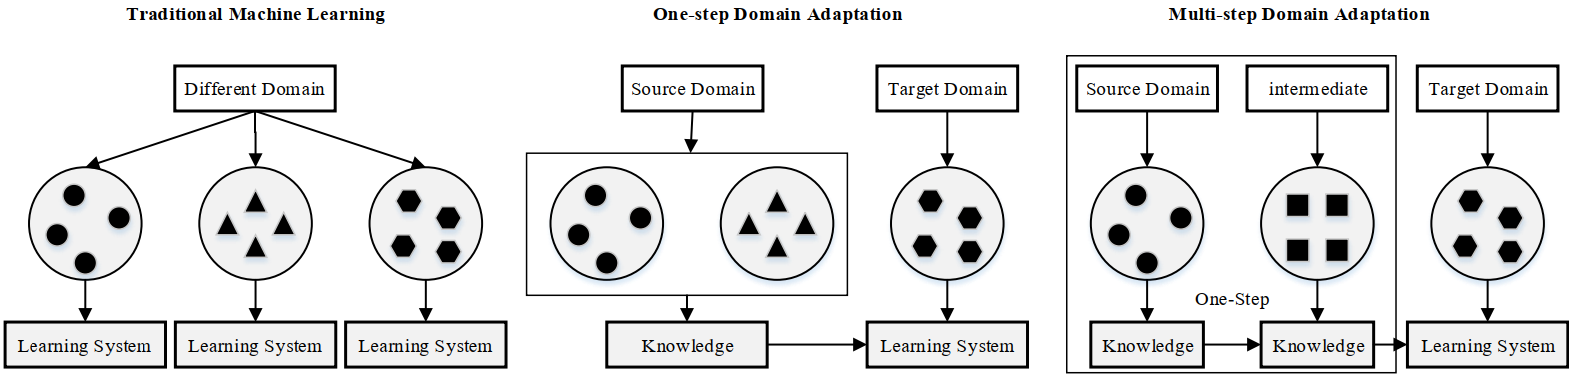
\includegraphics[width=\textwidth]{abbildungen/DAsteps.png}
  \caption{Knowledge transferring in types of Domain Adaptation \cite{deepDASurvey}: Different domains are involved differently in traditional machine learning (a), one-step DA (b) and multi-step DA. In traditional machine learning, each domains are used to train separately. In one-step DA the knowledge from source domains can be transferred directly to the target domain, whereas the multi-step uses another domain more similar to the target domain as an intermediate domain in the transfer.} 
  \label{fig:DAsteps}
\end{figure}

These differences between the domains present itself to a system as different distributions among the datasets - by changing the dataset, we also change the distribution of the data the system uses. This change of the distribution is called dataset shift and the datasets with different distributions are referred to as being from different domains. It is useful to understand how this happens before proceeding with solving this problem. In the next section, the cause of the different domains, the dataset shifts, will be discussed. 

\section{Dataset Shifts} \label{sec:datasetShifts}
In collecting data, there are many aspects that can in influence the characters of the data. To name examples related to image data, the lighting condition, for instance, can generally change the overall intensity of the pictures: the pictures take in a dark room will generally have lower intensity value than in the ones taken in sunlight regardless of which objects are captured. This shows an example of how the environment can change the underlying distribution of the input value. Another possible cause of a dataset shift is how the samples are selected to be in a dataset. It is understandable that a data collection is built up of the inputs of similar nature. This is referred to as the sample selection bias.

The insimilarities between the distributions, the dataset shifts, are categorized after the source of the shifts. In \cite{shiftinML} and \cite{shiftDataset}, the shift types are defined differently: in \cite{shiftinML} they are splitted after common causes of the shifts whereas in \cite{shiftDataset} they are splitted more generally after the change in probability distribution the shifts cause. Now, we will discuss different types of the dataset shifts according to \cite{shiftDataset}. To understand this, it must be mentioned first that the joint distribution $p(x, y)$, the probability that both x and y occur, can be calculated by:
	\begin{equation}\label{eq:jointXY}
			p(x, y) = p(x | y)p(y) = p(x | y)P(x)
	\end{equation}

According to this equation, the possible dataset shifts occur when $p(x)$, $p(y)$ or $p(x|y)$ changes which results in covariate shifts, prior shifts or concept shift respectively. 

\subsubsection*{Covariate Shifts}
The covariate shifts are caused by different distributions of the input between the domains whereas the conditional distributions of the output given the input are the same. This kind of shift is possible in a $X \to Y$ problem where y is dependent on x and occurs when $p(x)$ changes and the conditional probability $p(y|x)$ stays the same. This shift is a very commonly studied in the problem of domain adaptation. The covariate shifts include the case when the sampling is biased as mentioned above as the sample selection bias. This is the same as when the political survey is done to create a prognosis about the upcoming election, in an area where one political party invests more on running a campaign, the result would be more in favor of that party than in another area. The result of this area is not necessarily the real opinion of the majority of the people in that country. 
Another possible cause of the covariate shifts is when the data is missing from the collection which alters the probabilities of the remaining samples in the dataset. Having less representations of something could rise the probability of another thing in the same sample. The effect of the change is visualized in figure \ref{fig:covariateShiftPic}
\begin{figure}[tbh]
  \centering
    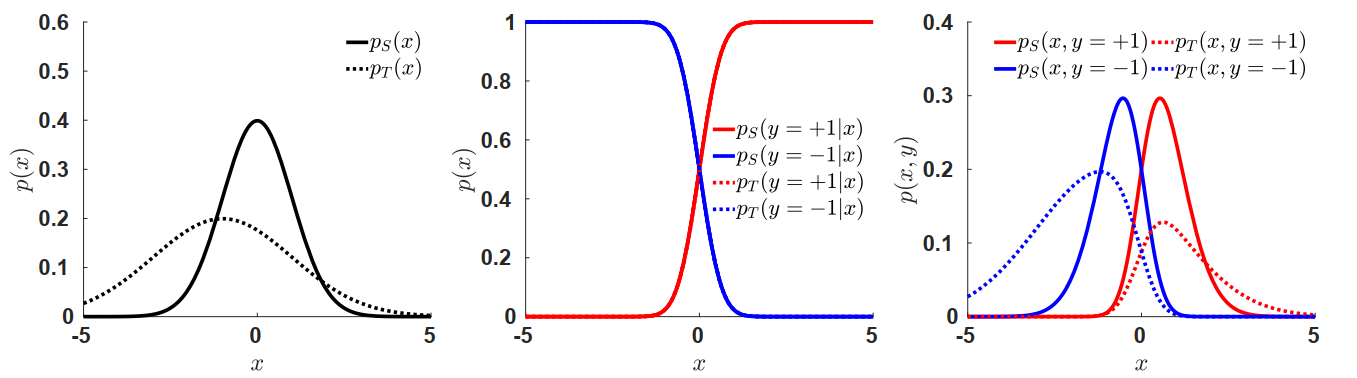
\includegraphics[width=\linewidth]{abbildungen/covariateShiftPic.png}
  \caption{Covariate Shift \cite{dataShifts}: There is a shift in the data distribution (Left) from the target (in the picture $p_T$) to the source (in the picture $p_S$) whereas the posterior distributions (Middle) are similar. As a result, the joint distributions (Right) are shifted.}
  \label{fig:covariateShiftPic}
\end{figure}

\subsubsection*{Prior Shifts}
The prior shifts, on the other hand, occur when the districution of the output changes, i.e., when $p(y)$ changes whereas the conditional probability $p(y|x)$ stays the same. This would also cause the joint distribution $p(x, y)$ to change. Practically, this shifts happen when the rule of the classification changes, for example, the level of toxic detected before it is classified as dangerous. If we take the sample from the same water, the composition of the water might not change but by changing the detection rule, the probability of the same water being toxic might alter if the threshold is changed. The visualization of the change in this distribution is to be seen in figure \ref{fig:priorShiftPic}.
\begin{figure}[tbh]
  \centering
    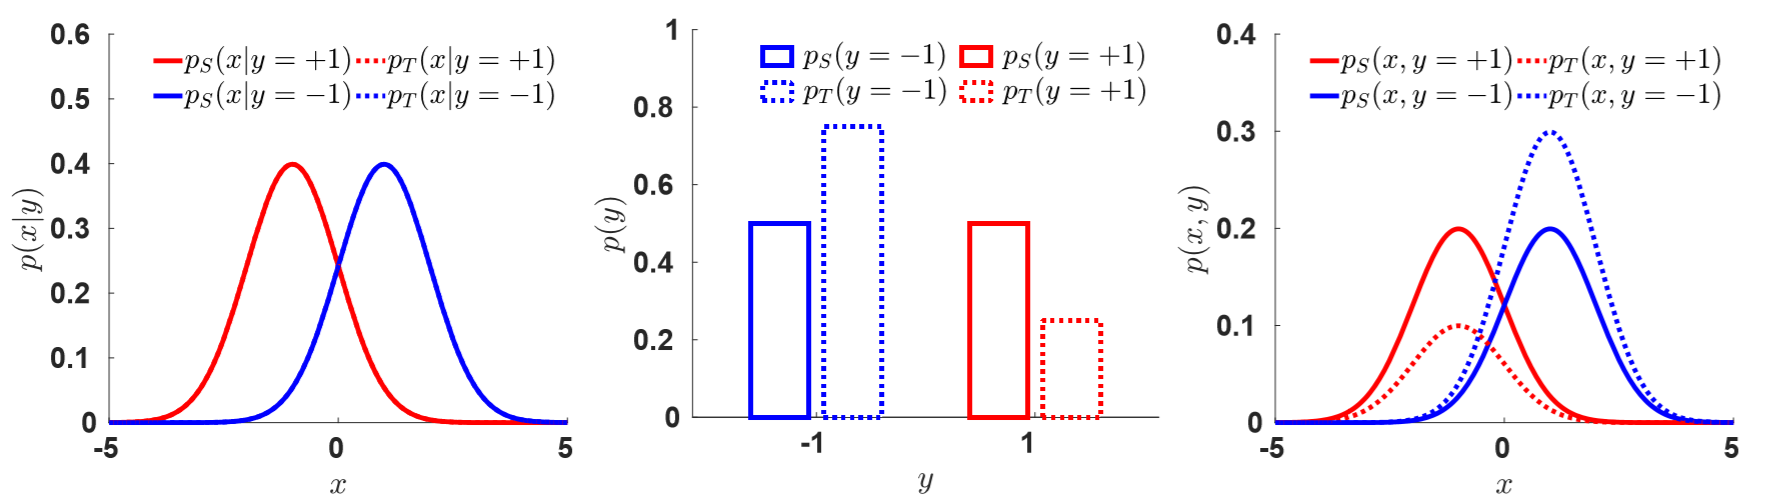
\includegraphics[width=\linewidth]{abbildungen/priorShiftPic.png}
  \caption{Prior Shift \cite{dataShifts}: The distributions of the positive and negative class label are similar within the training and testing set (Left) but due to the differences in probabilities $p_s \neq p_T$ (Middle), the joint probabilities are not equal in the testing set (Right)}
  \label{fig:priorShiftPic}
\end{figure}

\subsubsection*{Concept Shifts}
The concept shifts are different than two previous shifts. Here, the data distributions $p(x)$ and $p(y)$ are the same while the conditional distribution $p(x|y)$ changes. These shifts are common in reality since the nature of the conditions always changes. For example, forecasting weathers in different seasons also have different criterion. Figure \ref{fig:conceptShiftPic} illustrates this change and its effect on the joint distribution. 
\begin{figure}[tbh]
  \centering
    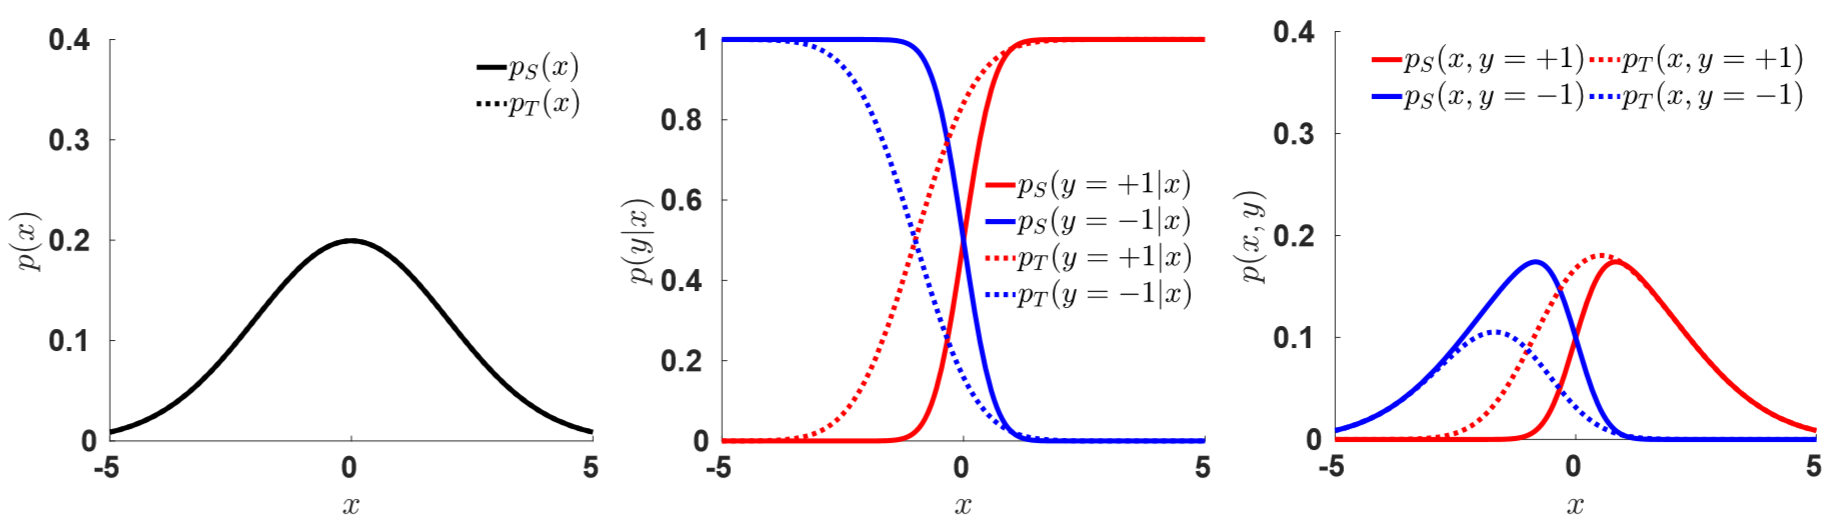
\includegraphics[width=\linewidth]{abbildungen/conceptShiftPic.png}
  \caption{Concept Shift \cite{dataShifts}: The data distributions in the source and the target set are the same (Left) but the shifts in $P_T(\vec{Y}|\vec{X})$ from that of the source target (Middle) cause a shift in the joint distribution (Right).} 
  \label{fig:conceptShiftPic}
\end{figure}

Due to these introduced shifts, datasets can have different data distribution. Since traditional classifier is not adaptive when it is trained on data from one domain and the testing is done on another domain, Domain Aadaptation (DA) is introduced to solve this problem. 

Mostly, the studied cases of domain adaptation assume complete source and target domains. However, there exist situations in which the involving domains are combinations of different domain. These scenarios are referred to as the Domain Mixture Scenario \cite{domainMixture}. In the next section, this particular scenario and its variations will be explained.


%Domain Mixture Scenario
\section{Domain Mixture Scenario} \label{sec:domainMixture}
Domain adaptation improves the performance of a network when the training is done on a dataset and the tasks should be performed on another dataset with different data distribution. This enables using similar data as the training data when the target data is entirely not available or just sparsely available. Ideally, the domain from which we have plenty of data should already contain a complete set of data i.e. samples of all classes we want to classify. If this is the case, the model will have a uniform data distribution to learn both the object representations and the domain information effectively. For example, creating 3D models can offer training images for all objects more efficiently than to actually capture the images of those objects from the real world. To be able to use these synthesized images as training data despite the real performance being planned for the real-world images, domain adaptation can be used to account for the different character of these images. Furthermore, it is also possible to have multiples classes serving as the training set. There might be, for instance, existing image collections of the same objects taken under different conditions that can be combined together to build up bigger training dataset than by using only one collection. 

In reality, a dataset might contain data from several different domains. For example, we might have images captured with different cameras or in different locations. It is also possible that each domain only contains parts of the possible classes and needs to be used together to create a dataset with complete class representations. This case of domain adaptation with multiple sources pose another challenges since there are now many data distributions in one source domain that should be approached differently from the situations with only a single domain acting as a source domain. To have an overview of this special situation, we will now briefly describe previous studies on these scenarios with many source domains.

\section*{Previous Experiments on Multi-source Domain Adaptation}
Most researches done on domain adaptation look into cases in which the domain transfer bridges one source domain to the target domain. However, if there are data from several domains available, using them all would give the model more useful data to work on than using just one domain. One possible way to use them is to combine them into one single source domain. By doing this, their differences might not be accounted for effectively enough \cite{multisourceDAsurvey}. Another possible way is to train several models solely on each one of the available domains, then to combine them into a model that can perform well on the new domain. \cite{multiDAclassi} developed the Domain Adaptation Machine (DAM) which learns to classify data in the target domain using classifiers pre-trained separately on the labeled samples from the source domains called auxiliary or source classifiers. The target classifier is optimized to make accurate predictions by adjusting weights applied on these auxiliary classifiers of each source domain. Its optimization aims to reduce the difference between the decision value of the target classifier and the source classifiers on the labeled source data. At the same time, the DAM also trains to minimize the decision error of the target classifier on the labeled target data if available. Figure \ref{fig:auxclassifiers} shows the structure of multi-source domain adaptation with separate source classifiers.

\begin{figure}[tbh]
  \centering
    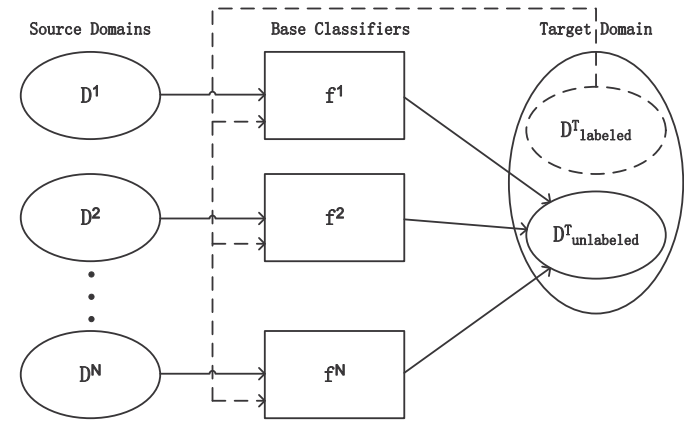
\includegraphics[width=0.8\textwidth]{abbildungen/multiDAclassi.png}
  \caption{Multi-source Domain Adaptation: Each classifier is trained on each available domain and labeled target data if possible. Then, they are combined to make accurate prediction on the unlabeled data in the target domain. \cite{multisourceDAsurvey}}
  \label{fig:auxclassifiers}
\end{figure}

The two mentioned methods require the domain labels of the data. In some situation in which we have a mixture of several unknown domains, for example, pictures from an internet search with many unknown origins. To support using these samples, \cite{multiDAcluster} proposed finding clusters representing domains in the data to acquire their domain labels. They also adapt a domain transformation method to the problem with multiple source domains. This original cross-domain transformaton \cite{multiDAcrosstrans} learns to find a transformation from a data point in a domain to the other and even works when not all the class samples in the target domain are in the training set - a very common situation when dealing with real-world data. 
 
In practice, the data serving as domain happens to lack elements of some classes and we may need to combine data from multiple domains to get a complete set of class representations as shown in figure \ref{fig:imsDA}. \cite{multisourceDA} published in 2018 also addressed insufficient exploration of the incomplete multisource transfer learning (IMTL) where none of the sources domain is complete. They proposed using low-rank transfer subspace to assist learning features from multiple domains. A subspace is a model suitable for describing the underlying characteristics of a dataset and a good way of realistically describing the nature a dataset is by using multiple subspaces \cite{subspaces}. Finding a shared subspace between source and target domains is one method of applying domain adaptation. With multiple sources, their different distributions must also be taken into account. Further from finding a domain-free subspace by finding low-dimensional features representing different classes, they reconstruct the missing class data of each source domain through this shared subspace with the information from the complete target domain - they learn from each other in both ways. 

Partly, the experiments in \cite{multiDAcrosstrans} and \cite{multisourceDA} assume, similarly to the domain mixture scenario, incomplete domains involving in the training phase - the datasets shown during the training have labeled samples of only subsets of all the competing classes. A difference is that \cite{multiDAcrosstrans} also include some labeled samples of the target which are not labeled at all in the domain mixture scenario. However, \cite{multisourceDA} also includes only unlabeled target samples. A crucial variation in our experiments, similar to \cite{domainMixture}, is the investigation on the varying ratio of the labeled samples to the unlabeled samples from different domains in the mixture. 

\begin{figure}[tbh]
  \centering
    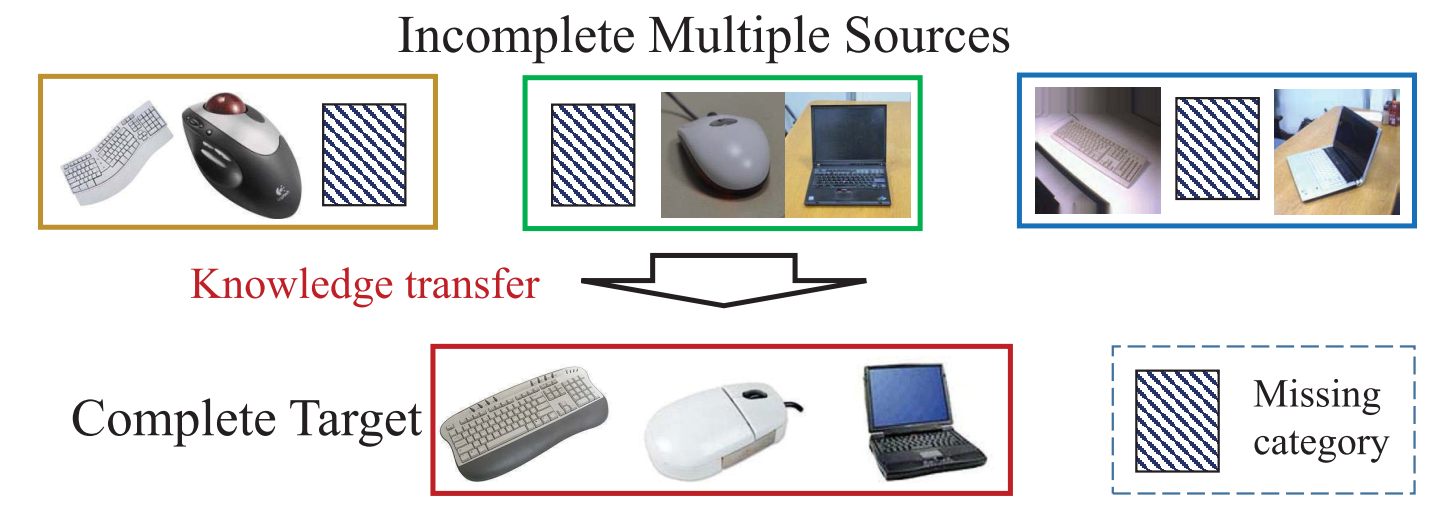
\includegraphics[width=\textwidth]{abbildungen/IMS-DA.png}
  \caption{Domain Adaptation with Incomplete Multiple Sources: Sometimes, we must combine multiple domains to have complete samples of all possible classes existing in the target domain. \cite{multisourceDA}} 
  \label{fig:imsDA}
\end{figure}

In this thesis, we investigate the scenario of domain adaptation as present in \cite{domainMixture} where there are supervised samples of all competing classes but they are not all from the same domain. This scenario actually represents the reality. A complete image collection of objects taken under the same condition, with the same camera model or pictures drawn or generated in the same style are created mostly for researches. In reality, we might find pictures of some objects taken under one condition and others taken under another. \cite{domainMixture} is also motivated by several operating house robots which serve in different areas in the house. A robot responsible for the kitchen might have captured a picture of a knife and a mixer while a robot serving in the bedroom might have pictures of a pillow the first one has never captured. On the other hand, the dog roaming around the house probably has been captured by both. It’s also realistic to imagine that both rooms have different light setting and the robots have different models of camera, then the pictures of each object will also come from different domains. Then, it is also possible that the images of some objects under a capturing condition are already labeled and others are not. Possibly and ideally, all the objects might appear in all the domains involved. As we can see, there are many possibilities of how the situation of the image collection usable as a training dataset can be.   

Of interest are the cases in which there is a complete set of supervised samples representing every possible classes we can use as a training set. However, these supervised samples are not all from the same domain and none of the domain has supervised samples of all the classes - the samples from both domains must be mixed in order to create a full representation of the classes. In \cite{domainMixture}, two versions of this scenario are investigated:  
\subparagraph*{Complete Domain Mixture: } Here, apart from the supervised data from some classes, the domains also have unsupervised samples of the remaining classes. In other words, all the domains have a complete set of samples with all the classes but they are only partly supervised.      
\subparagraph*{Sparse Domain Mixture: } In this variation, combining the supervised samples from all the domains still yield a set with all the classes but each domain has unsupervised samples of only parts of the missing classes. 
These two different scenarios of domain mixture are shown in Figure \ref{fig:scenarioDA}. 

\begin{figure}[tbh]
  \centering
    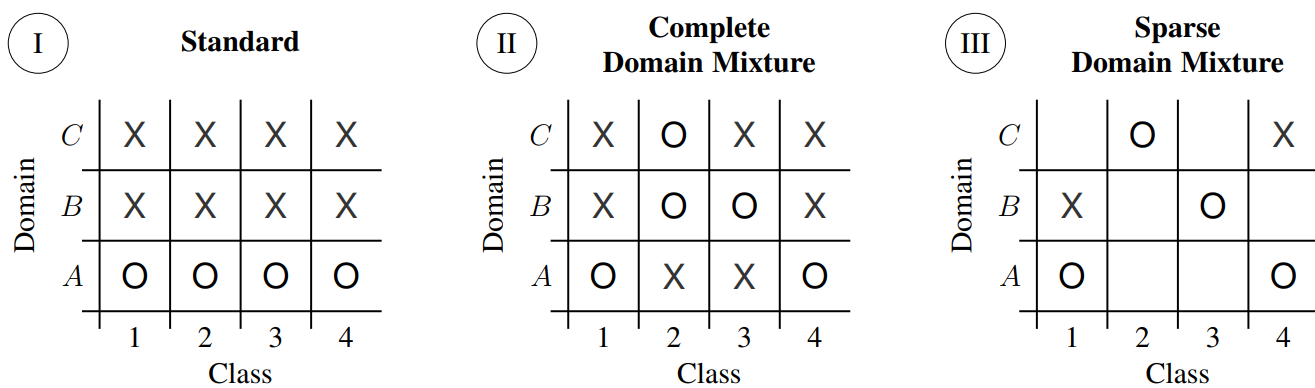
\includegraphics[width=\textwidth]{abbildungen/scenarioDA.png}
  \caption{Different Domain Mixture Scenarios \cite{domainMixture}: Present classes in the domains (A, B, C) are different in each scenario. The classic case of domain adaptation (left) is when we have a complete set of supervised data from one domain and want to learn to transfer the knowledge to other unsupervised domains which are also completed. The domain mixture scenarios also have supervised samples from all competing classes but only the complete one (middle) also has unsupervised samples from the missing domain-class combinations whereas the sparse one (right) lacks some combinations entirely.}
  \label{fig:scenarioDA}
\end{figure}

These scenarios are challenging since the objects are known to the network only in one variation from a domain, and some objects in other variation. The network has less information on what is domain-specific or what is object-specific. Intuitively, if we take different backgrounds as different domains and we want to tell what object is in the pictures, we would have to know what identifies the object and what comes from the background. We would make an assumption to what the object is, then we would look for the same object with different background to be able to confirm our assumption. In the domain mixture scenario, the model might only have seen an object and been told by the label what object it sees, then it would try to learn which features signalize the object. However, since it only has labeled pictures of that object with one background, it cannot directly compare what features are common when the backgrounds are different. Instead, it must try to extract background-specific features from the mixed data available and then learn aspects of the image that is independent from the backgrounds which should be relevant to the object itself. This is also already proposed in a theory on domain adaptation that the domain-irrelevant representations enable the best condition for a domain transfer the classifier needs  \cite{DArepres}.

With the knowledge about the domain adaptation and especially the domain mixture scenario, the next section will describe the DSN, how it applies domain adaptation with its components and why it might be a good choice to tackle these scenarios.
\chapter{Domain Separation Networks} \label{ch:dsn}
Increasingly, there are scenarios where we, purposely or inevitably, use data from different domains to train and use a system. Using domain adaptation can help improving the performance of the system as already proven by several previous attempts with various methods \cite{DAGanin, DASurvey}. The Domain Separation Network \cite{DSN} is a neural network that applies domain adaptation effectively and even surpassed some of the previous methods. 

There are many strategies of domain adaptation, e.g. by learning domain-invariant features or by mapping source to target domain. The DSN, like some other architectures, learns so that the representations of the images from source and target domain are similar to each other - the classifier can classify objects independently from its domain. The crucial addition to DSN is that it learns both the components shared by source and target domains and the components only related to a single domain. This way, the network would not mix up the noise coming from shared components of the domains to the representation related to the actual objects that are also common to all domains. 

To better understand DSN, we first need to understand its building blocks and foundations. In this chapter, its own structure, the loss functions involved in its training and the components used in this architecture, which are crucial to the experiments, such as Domain Adversarial Neural Networks (DANN) \cite{dannGanin}, will be discussed in detail. The first section begins with the main structure of the Domain Separation Networks.
 
\section{Structure of Domain Separation Networks} \label{sec:dsnStruct}

\begin{figure}[tbh]
  \centering
    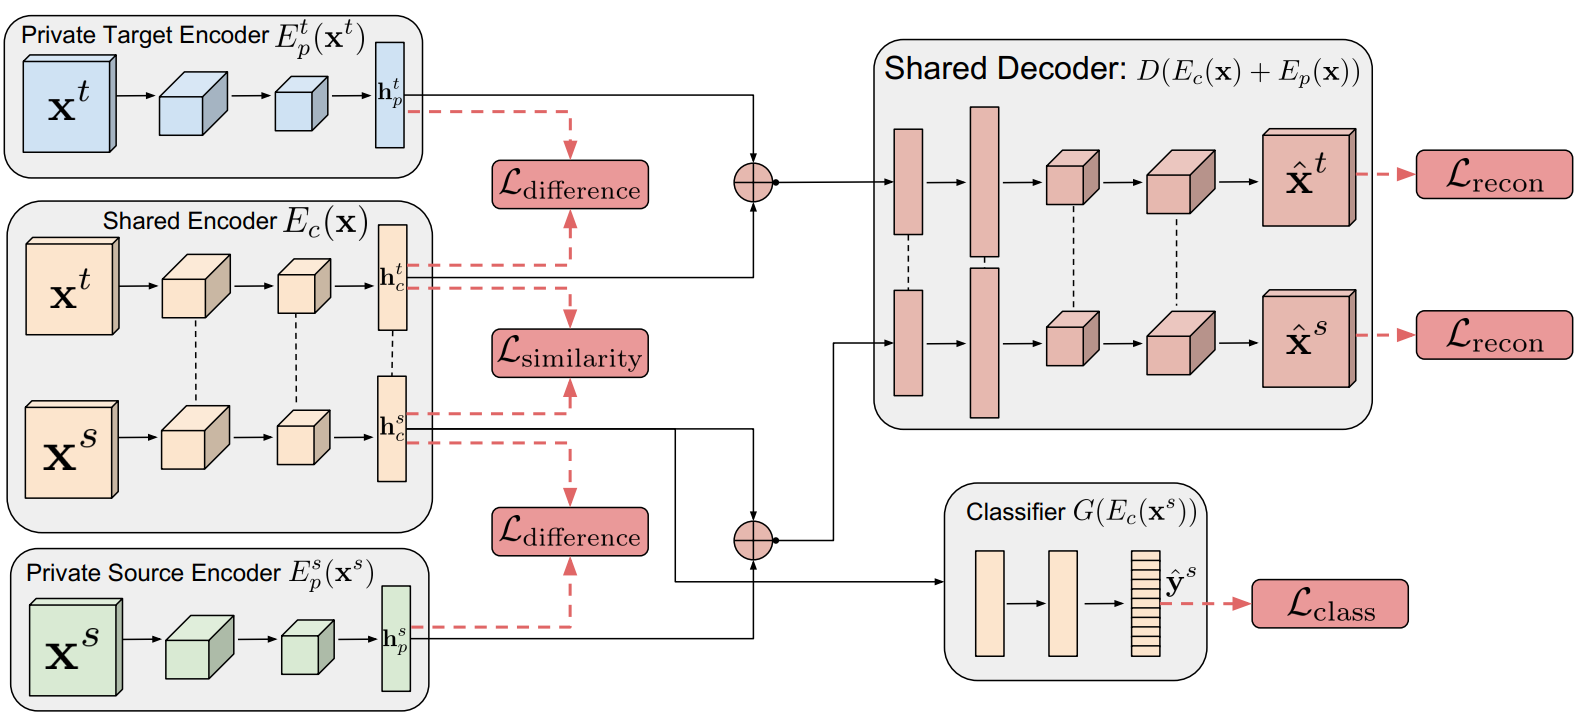
\includegraphics[width=\textwidth]{abbildungen/DSN.png}
  \caption{Main Structure of Domain Separation Networks: A DSN contains private encoders for both domains, ${E_p}^t(x^t)$ for the target domain and ${E_p}^s(x^s)$ for the source domain, a shared encoder $E_c(x)$ creating representations shared across the domains, shared decoder that reconstructs both private representations and evaluate the loss and finally, the classifier $G\left(E_c(x^s)\right)$ that classifies the images based on supervised input images from the source domain.}
  \label{fig:DSN}
\end{figure}

Figure \ref{fig:DSN} shows the structure of the DSN. The network is built up with its private encoders responsible to the source and the target domain, the shared encoder handling the shared representation, the shared decoder that validates the private representations by calculating reconstruction losses, and the classifier trained on the labeled images from the source domain. 

A DSN supports domain adaptation by separately creating representations of the images specific to just the source or target domain, as well as representations shared by both domains. These representations are extracted by the encoders whose functions are described in Section \ref{sec:autoencoders}. Then, since the private representations should be different from each other as possible and should contain generally the characteristics of each domain, the authors add reconstruction losses to ensure that the private representations and the shared representations created by the private encoders are still relevant to the domain it represents. The goal of this separation is to enable the classifier to train on the shared representation, which should be classifiable independently from the domains, without contamination from the representations unique to any of the domains. 

To train the network, the authors use an overall loss function containing four different losses: task loss, reconstruction loss, difference loss, and similarity loss. Since the DANN is used to induce the similarity loss, its structure and function must be explained first before these loss functions are explained in detail in Section \ref{sec:dsnLoss}.

%DANN
\subsection{Domain Adversarial Neural Networks} \label{sec:dann}
The domain adversarial neural network (DANN) \cite{dannGanin} is inspired directly from the idea of domain adaptation suggesting that the prediction made on representation with unclear domain of origin - neither source nor target - is the most effective in tasks with domain transfer \cite{DArepres}. Therefore, the DANN is modeled so that its hidden layer is optimized to be good at classifying the inputs but to be bad at distinguishing their domain which makes this network adversarial to itself. 

\begin{figure}[tbh]
  \centering
    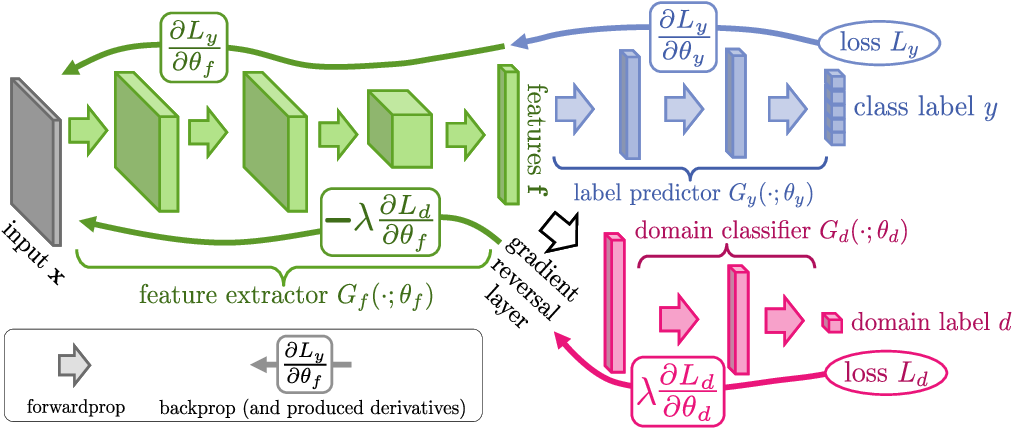
\includegraphics[width=\textwidth]{abbildungen/dann.png}
  \caption{Domain-Adversarial Training \cite{dannGanin}: In the domain-adversarial training of a network, the features are first extracted from the input. Then these extracted features are both used to train the label predictor to be able to make accurate predictions of the class of the input and, at the same time, to try to confuse the domain classifier to make bad predictions about the domain of the input. Both classifiers are trained adversarially against each other.}
  \label{fig:dann}
\end{figure}

As describe above, the DANN has to learn to classify images as accurately as it can while not classifying their domains well. The accuration of the classification can be measured by a loss function that indicates how far the prediction is from the reality. To classify the image, it learns to minimize the classification loss $\mathcal{L}(\bm{f}(\bm{x}), y)$ defined using the negative log probability as in equation \ref{eq:neglogDANN} where $f(\bm{x})$ is the predicted probability of $x$ being in class $y$ defined by the softmax function as in \ref{eq:softmaxDANN} 
 	\begin{equation} \label{eq:neglogDANN}
			\mathcal{L}(\bm{f}(\bm{x}), y) = log\frac{1}{f_y(\bm{x})}
	\end{equation} 	
	\begin{equation} \label{eq:softmaxDANN}
			\bm{f}(\bm{x}) = softmax(\bm{c} + \bm{V}h(x)),
			softmax(\bm{a}) = \left[\frac{1}{1+exp(a_i)}\right]_{i=1}^{|\bm{a}|}
	\end{equation}
	\begin{equation} \label{eq:represDANN}
			\bm{h}(\bm{x}) = sigm(\bm{b} + \bm{W}h(x)), 
			sigm(\bm{a}) = \left[\frac{exp(a_i)}{\overset{|\bm{a}|}{\underset{j=1}{\sum}}exp(\bm{a}_j)}\right]_{i=1}^{|\bm{a}|}
	\end{equation}
$h(\cdot)$ in \ref{eq:represDANN} can be viewed as the internal representation of the neural network responding to the $m$ labeled source data: $\bm{h}(S) = \left\{\bm{h}(\bm{x}_i^s)\right\}_{i=1}^m$. Then, $\bm{b}, \bm{W}$ are the network parameters responsible for creating the representations and $\bm{c}, \bm{V}$ are parameters of the classifier similar to $\bm{b}, \bm{W}$ 

Then we have unlabeled data from the target domain with $n$ samples and the representation $\bm{h}(T) = \left\{ \bm{h}(\bm{x}_i^t)\right\}_{i=1}^{n}$. Combining the empirical $\mathcal{H}$-divergence \cite{DArepres, H-Kifer}, a method to measure the difference of data distribution, measuring the difference between the representations $\bm{h}(S)$ and $\bm{h}(T)$ \eqref{eq:hDiv} and a logistic regressor predicting the probability of a given output being from the source domain or target domain, $z = 1$ or $z = 0$ accordingly \eqref{eq:logReg}:
 	\begin{equation} \label{eq:hDiv} 
			\hat{d}_{\mathcal{H}} = 2\left(1 - \underset{min}{\eta \in \mathcal{H}}\left[\frac{1}{m}\underset{i=1}{\overset{m}{\sum}}I\left[\eta \left(\bm{h}\right(\bm{x}_i^s)) = 1\right] + \frac{1}{n}\underset{i=1}{\overset{n}{\sum}}I\left[\eta \left(\bm{h}\left(\bm{x}_i^t\right)\right) = 0\right]\right]\right) 
	\end{equation} 
	\begin{equation} \label{eq:logReg} 
			p(z =1 | \Phi) = o(\Phi) = sigm(d+\bm{u}^T\Phi), \Phi \in \left\{\bm{h}(\bm{x}_i^s), \bm{h}(\bm{x}_i^t)\right\}
	\end{equation} 
with weights and biases of the neurons $\bm{u}, d responsible for the domain regressor$.

Regarding both parts, the classifier and the domain regressor, the DANN tries to minimize the loss of the first and to maximize the confusion in the second. The optimization problem its training has to solve is as follow:
	\begin{equation} \label{eq:optDANN} 
			\underset{\bm{b}, \bm{c}, \bm{V}, \bm{W}}{min}\frac{1}{m}\underset{i=1}{\overset{m}{\sum}}\mathcal{L}\left(\bm{f}\left(\bm{x}_i^s\right), y_i^s\right) + \lambda\underset{\bm{u}, d}{max}\left[\left(-\frac{1}{m}\underset{i=1}{\overset{m}{\sum}}\mathcal{L}^d\left(o\left(\bm{x}_i^s\right), 1\right) - \frac{1}{n}\underset{i=1}{\overset{n}{\sum}}\mathcal{L}^d\left(o\left(\bm{x}_i^t\right), 0\right)\right)\right]
	\end{equation} 


% Loss Functions
\section{Loss Functions of Domain Separation Networks} \label{sec:dsnLoss}
The loss function gives information about how well the network can already classify the given data. It can be defined to evaluate the error of the network and to lead the learning in the direction we want. The total loss of DSN is defined as follow 
	\begin{equation} \label{eq:lossesDSN}
			\mathcal{L} = \mathcal{L}_{Task} + \alpha \mathcal{L}_{recon} + \beta \mathcal{L}_{difference} + \gamma \mathcal{L}_{similarity}
	\end{equation}
where $\alpha$, $\beta$ and $\gamma$ are coefficients for the reconstruction loss $\mathcal{L}_{recon}$, the difference loss $\mathcal{L}_{difference}$ and the similarity loss $\mathcal{L}_{similarity}$ respectively. 

Now that we know all the necessary components and the overall loss function, the definitions of all the loss functions will be declared and explained.

\subsection*{Task loss}
For the main task of image classification, we want the network to make accurate predictions regarding the class of an image. If there is a dog in a picture, the network should predict that it is highly probable that a dog is in that picture. If the prediction indicates otherwise, there must be a noticeable consequence. Having the ground-truth information, the labeled data, one way to do this is to define a loss function indicating the amount of errors in the predictions: the further the predictions are from the reality, the bigger the loss is. The authors use the negative log-likelihood as defined in equation \eqref{eq:loglikeFnc} for the task loss $\mathcal{L}_{Task}$.
	\begin{equation} \label{eq:loglikeFnc}
			\mathcal{L}_{Task} = -\overset{N_s}{\underset{i = 0}{\sum}}y_i^s \cdot log {\hat{y}_i}^s
	\end{equation}

where  $y_i^s$ is the class label in one-hot encoding form for input $i$ and ${\hat{y}_i}^s$ the softmax prediction of the classifier $G\left(E_c(x^s)\right)$.

The negative log-likelihood is bigger, when the predicted probability of an image belonging to a wrong class is high or when the predicted probability of the right class is low. Therefore, the network learns to adjust its parameters to minimize this loss - to make more accurate predictions. It must be note that this classification loss is calculated based only on the labeled source data offering ground-truth information.

\subsection*{Difference Loss}
The difference loss encourages the private encoders and the shared encoders to be different. They should capture other aspects of the same input from both domains. Here, the authors use a soft subspace orthogonality constraint between the two representations of each domain. The difference loss is defined as:
	\begin{equation} \label{eq:difflossFnc}
			\mathcal{L}_{difference} = \Vert {H_c^s}^T{H_p^s}{\Vert_F^2} + \Vert {H_c^t}^T{H_p^t}{\Vert_F^2}
	\end{equation}
	\begin{equation} \label{eq:frebFnc}
			\Vert A {\Vert_F} = \sqrt{\overset{m}{\underset{i = 1}{\sum}}\overset{n}{\underset{j = 1}{\sum}}|a_{ij}|^2}
	\end{equation}

where ${H_c^s}$ and ${H_p^s}$ are matrices which respectively has the hidden shared representations $h_c^s = E_c(x^s)$ and the private representation $h_p^s = E_p(x^s)$ of the samples from the source domain as their rows and ${H_c^t}$ and ${H_p^t}$ are matrices with the hidden shared representations $h_c^t = E_c(x^t)$ and the private representation $h_p^t = E_p(x^t)$ of those from the target domain as their rows respectively. $\Vert \cdot {\Vert_F^2}$ is the squared Frobenius Norm with \eqref{eq:frebFnc} as definition.

\subsection*{Reconstruction Loss}
DSN has a structure generating domain-specific representations which are held apart from the shared representation by the difference losses. To ensure that the private representations are not trivial, the authors also add reconstruction loss using scale-invariant mean squared error $\mathcal{L}_{si}$\_${mse}$ as defined in equation \eqref{eq:reclossFnc} and \eqref{eq:si_mse}
	\begin{equation} \label{eq:reclossFnc}
			\mathcal{L}_{recon} = \overset{N_s}{\underset{i = 1}{\sum}}{\mathcal{L}}_{si\_{mse}}(x_i^s, {\hat{x}_i}^s) + \overset{N_t}{\underset{i = 1}{\sum}}{\mathcal{L}}_{si\_{mse}}(x_i^t, {\hat{x}_i}^t)
	\end{equation}		

	\begin{equation} \label{eq:si_mse}
			\mathcal{L}_{si\_{mse}}(x_i^s, {\hat{x}_i}^s) = \frac{1}{k} \Vert x - \hat{x}{\Vert_2^2} - \frac{1}{k^2} ([x - \hat{x}] \cdot 1_k)^2
	\end{equation}

	\begin{equation} \label{eq:L2Fnc}
			x = \left(\begin{array}{c} x_1\\ x_2\\ \vdots \\ x_n \end{array} \right),
			\Vert x {\Vert_2^2} = \sqrt{\overset{n}{\underset{k = 1}{\sum}}{|x_k|}^2} \\
			\mathcal{L}_{si\_{mse}}({x_i}^s, {\hat{x}_i}^s) = \frac{1}{k} \Vert x - \hat{x}{\Vert_2^2} - \frac{1}{k^2} ([x - \hat{x}] \cdot 1_k)^2
	\end{equation}

where $k$ is the pixel number in input $x$, $1_k$ a k-dimensional vector filled with ones, and $\Vert \cdot {\Vert_2}^2$ is the squared $L_2$-norm defined as in equation \ref{eq:L2Fnc}

The authors also proved that by using the scale-invariant mean squared error, better performance can be aimed [DSN]. This is because the scale-invariant mean-squared error allow the DSN to concentrate on reconstructing the shape of the object without being punished on wrong value of intensity or absolute color whereas the traditional mean-squared error also punishes wrong scaling of the output despite the object being reproduced correctly. 

Pictures can also be regenerated back according to the diffrerent representations as shown in Figure \ref{fig:reconImg}

\begin{figure}[tbh]
  \centering
    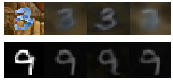
\includegraphics[width=0.6\textwidth]{abbildungen/reconPic.png}
  \caption{Reconstructed Images: These are the images reconstructed from different representations. Respectively from the left to the right of each row, the first one is the original image, the second is reconstructed from both the shared and private representations, the third is from only the shared representations and finally, the fourth is constructed only after the private representations.}
\label{fig:reconImg}
\end{figure}

\subsection*{Similarity Loss}
For the shared representations, both the representations of the samples from the source domain and of the samples from the target domain should be similar. In that way, the classifier can train on the common representations that are domain-independent. To induce this in the model, the authors chose two ways to define the similarity loss: the domain adversarial similarity loss and the maximum mean discrepancy. 

\paragraph*{i. Domain Adversarial Similarity Loss} This adversarial learning is also known in Domain Adversarial Neural Network (DANN) \cite{DAGanin} described previously in \ref{sec:dann}. It is a way to induce the similar representations of both domains is by learning to create representations that confuse a domain classifier. On one side, there is a domain classifier learning to predict the domain of the samples from the encoded representations. On the other side, the representations should be created so that the classifier cannot reliably predict their origin domain. 

To enable this contrary behavior in the model, the Gradient Reversal Layer (GRL) is used. The GRL $Q(f(u))$ is defined as the identity function $f(x) = x$ but has the reversed gradient direction, that is: 
	\begin{equation}
			Q(f(u)) = f(u)
	\end{equation}

	\begin{equation}
			\frac{d}{du}Q(f(u)) = -\frac{d}{du}Q(f(u)) = -\frac{d}{du}f(u)
	\end{equation}

Formally, there is the domain classifier $Z(Q(h_c);\bm{\theta}_z) \rightarrow \hat{d}$ making prediction on the domain $\hat{d} \in \left\{0, 1\right\}$ of the input sample x through a shared representation vector $h_c = E_c(x; \bm{\theta}_c)$. While $\bm{\theta}_z$ is adjusted to improve accuracy of the classifier in predicting the domain of the encoded images, the parameters $\bm{\theta}_c$ are optimized to create representations that the classifier cannot classify accurately. 

\paragraph*{ii. Maximum Mean Discrepancy} 
Maximum Mean Discrepancy (MMD) is a kernel-based method proposed by \cite{mmdOrig} to find out if the two drawn samples are from the same distribution. This problem is also known as the two-sample problem and is defined formally as: given $X := \left\{x_1, \cdots, x_m\right\}$ drawn from $p$ and $Z := \left\{z_1, \cdots, z_m\right\}$ drawn from $q$, we want to test whether $p=q$ \cite{mmdbio}. 

Generally, MMD is the maximum difference of the mean function value $f(x)$ and $f(y)$ on samples $X$ and $Y$. Since we want to concentrate on the usage of the MMD, the derivation of the equation \eqref{eq:mmddsnFnc} used in the DSN will not be explained in detail here but can be found in \cite{mmdOrig}. Here, the authors used the biased statistic for the squared population MMD to measure the difference between the shared representations of the samples from the source domain $\bm{h}_c^s$ and the shared representations of those from the target domain $\bm{h}_c^t$:
\begin{equation}\label{eq:mmddsnFnc}
			\mathcal{L}_{similarity}^{MMD} = \frac{1}{(N^s)^2}\overset{N^s}{\underset{i, j = 0}{\sum}}k(\bm{h}_{ci}^s, \bm{h}_{cj}^s) - \frac{2}{N^sN^t}\overset{N^s, N^t}{\underset{i, j = 0}{\sum}}k(\bm{h}_{ci}^s, \bm{h}_{cj}^t) + \frac{1}{(N^t)^2}\overset{N^t}{\underset{i, j = 0}{\sum}}k(\bm{h}_{ci}^t, \bm{h}_{cj}^t)
	\end{equation} 
with a positive definite kernel function $k(\cdot, \cdot)$. The author chose a linear combination of multiple radial basis function kernel defined as: 
\begin{equation}\label{eq:rbfFnc}
			k(x_i, x_j) = \sum_n \eta_n exp\left\{-\frac{1}{2\sigma_n}\Vert x_i - x_j\Vert^2\right\} 
	\end{equation} 
with the standard deviation $\sigma_n$ and the weight of the $n^{th}$ kernel $\eta_n$  

After the introduction to the components of the DSN, we can summarize it as follow: the encoders, the decoders and the classifier along with the difference loss, the reconstruction loss, and the similarity loss  enable the DSN to be trained to apply domain adaption to image classification. The private encoders for the source and target domains $E_p^s(\bm{x}^s)$ and $E_p^s(\bm{x}^s)$ create the private source representations $\bm{h}_p^s$ to be different to the shared representations also built from the source $\bm{h}_c^s$, and the private target representations $\bm{h}_p^t$ to also be different to the shared representations from the target domain $\bm{h}_c^t$. The differences between these representations are induced by the difference loss $\mathcal{L}_{difference}$. At the same time, the similarity loss $\mathcal{L}_{similarity}$supports the similarity between both shared representations $\bm{h}_c^s$ and $\bm{h}_c^t$ on which the classifier can train effectively according to a theory to domain adaptation described in Section \ref{ch:domainAdaptation}. Then, to prevent the private encoders from creating trivial solutions trying to be different from the shared representations, the reconstruction loss is added to ensure that the encoded matrices can still be decoded back to images resembling the ones from their domain of origin. Finally, the classifier trains to classify image by learning from the domain-invariant representations created by the share encoders as mentioned before. Their cooperation is depicted in figure \ref{fig:DSN}.

\section{Previous Experiments with Domain Separation Networks} 
\subsection*{Domain Separation Networks (DSN)} In the original paper, the authors are interested in the DSN's performance on a real-world dataset when it is trained on a synthetic data. This scenario involves domain transfer from a domain with clear representation of data to the noisy one. The dataset they used are MNIST, white digits on black backgrounds, MNIST-M created by inverting color of the images in MNIST partially. They carry experiments using DSN trained on MNIST \cite{mnist} to test on MNIST-M \cite{mnist-m}, Synthetic Digits to the Street View House-Number Set (SVHN) \cite{svhn}, SVHN to MNIST, Synthetic Signs to the real-world dataset of traffic signs (GTSRB) \cite{gtsrb} and synthetic objects to LINEMOD \cite{linemod}. Samles from some of these datasets can be seen in figure \ref{fig:datasets}. 

As they reported, they achieved the highest classification accuracy when using the DSN with the DANN as similarity loss. This shows the effectiveness of their domain adaptation method separating domain-specific information from the shared representation.

\begin{figure}[tbh]
  \centering
    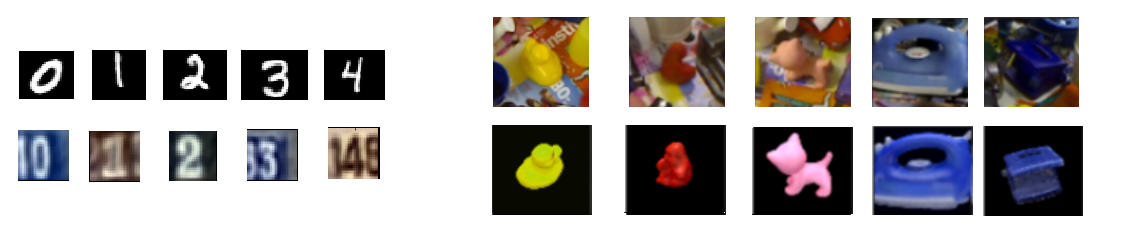
\includegraphics[width=\textwidth]{abbildungen/datasets.png}
  \caption{Synthetic Images and Real-world Images: On the left, samples from the MNIST dataset (upper left) and from the SVHN (lower left) are shown. We can see that the first has cleaner look with clear digits and uniform background while the real-world house numbers have blurry appearance. Similarly on the right, the synthetic objects (upper right) has black background and the objects from the LineMod (lower right) are almost lost among the background, as pictures from the real scene could look like.}
  \label{fig:datasets}
\end{figure}

\subsection*{Speech Recognition with DSN \cite{dsnspeech}} 
The DSN has found not only application in computer vision, but also in speech recognition. In this paper, it is used in an unsupervised domain adaptation problem to recognize speeches with only a sequence of speech with labels. They also train the network on a clean speech data and test on the noisy speech data. Also this work reports a good average performance of the DSN in the speech recognition. Since this is not exactly our scope, we will not go in the detail of this work. Further information can be found in \cite{dsnspeech}. 

After knowing the components and functions of the DSN in this section, how it extracts features specific to each domain and hold it far from each other and at the same time extract shared aspects of both domains, it is imaginable that the domain separation network would be a suitable choice for this situation.  the DSN has encoders which learn to explicitly extract the domain-specific information on both domains. This way, it can really tell both domains apart even if they are mixed together. Besides, by extracting the private representations of each domain, it can make clearer representations of the objects even though it has not seen labeled image of that object from another domain before. The DSN extracts the characters of each domain and create the representations freed from the domains on which its classifier can learn about the objects very precisely without noises from both the differences an the similarities between the domains. In the next section, we will introduce our experiments using this network and present our results.

In our experiment, the complete domain mixture scenario, with both domains having samples from all classes, is investigated. The main difference to \cite{domainMixture} is that another neural network architecture is used to observe the effect of this mixture. While they train a DANN on these scenarios in \cite{domainMixture}, the DSN is used in this thesis. Practically, the DSN also includes the DANN to create domain-free representations, then additionally create domain-specific representations. By using another neural network, we can also see if the interference of the mixture they measure is specific to the choice of the model or not and how. The experiments will also be carried with different number of classes from which each domain has supervised samples to see how the overlapping of the data of the same object between the domains influences the performance of the model. The next section will describe our experimental setup further in details.
\chapter{Experiments on Domain Mixture Scenario with Domain Separation Networks} \label{ch:experiment}
In the last section, we covered the scenarios in focus of this thesis: the complete domain mixture scenario. This is the situation in which the source domain is consisted of multiple domains mixed together and, as the name implies, all the domains have complete representations of all the classes. However, the domains are only complete but none of the involving domain is completely supervised, i.e., only samples of some classes represented in a single domain come with labels. Only through mixing those domains together do we achieve a source domain with complete supervised representations of the classes. The goal of the domain adaptation in this case is to train a network using this mixed source domain to perform a classification task on samples in these domains that it only has seen unsupervisedly without labels. In our experiment, we use the setup with only two domains involved and the mixture of them creates the source and target domain. First, the datasets used will be introduced before necessary definitions and notations of the experiments are summarized

\paragraph*{Datasets} For our experiments, we use the MNIST and the MNIST-M dataset. The MNIST \cite{mnist} dataset contains grayscale pictures of handwritten digits from 0 to 9 with 60,000 training images and 10,000 test images. The MNIST-M \cite{mnist-m} is created by inverting colors of the MNIST images by cropped images from the Berkeley Segmentation Data Set and Benchmarks 500 (BSDS500) \cite{bsds500}. It contains 59,001 training images and 9,001 test images. Due to the color modification, these two datasets represent two different domains. In this section, we will refer to the MNIST dataset and the MNIST-M dataset as $S$ and $M$ respectively to conform with \cite{domainMixture}. Samples from these datasets are shown in Figure \ref{fig:mnistmnistm}

\begin{figure}[tbh]
  \centering
  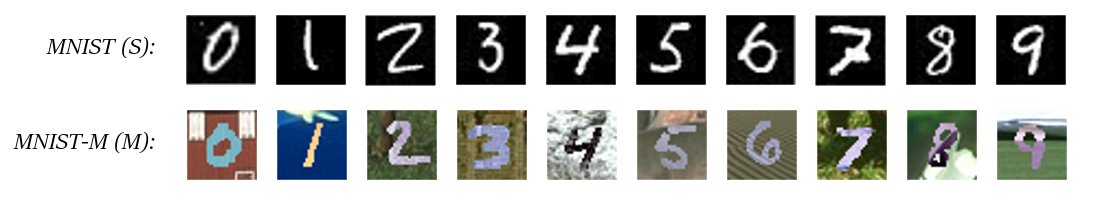
\includegraphics[width=0.8\textwidth]{abbildungen/mnistmnistmText.png}
  \caption{MNIST and MNIST-M: MNIST contains grayscale images while MNIST-M contains color images. They represent different domains.}
  \label{fig:mnistmnistm}
\end{figure}

\section*{Notations and Definitions}
\paragraph*{Source Domain $\mathcal{D}_S$} The source domain is the mixture of S and M with $m$ classes of supervised samples. For the complete supervised training samples, we use $m \in \{5, 6, 7, 8, 9\}$. More details will be discussed further in the next section.
\paragraph*{Target Domain $\mathcal{D}_T$} The target domain is also the mixture of S and M which is involved only unsupervisedly in the training and is used to perform the evaluation of the trained model.
\paragraph*{Training Parameters} According to the total loss function in \eqref{eq:lossesDSN} mentioned in section \ref{ch:dsn}, the DSN has the parameters: $\alpha$ controlling the reconstruction loss, $\beta$ controlling the difference loss and $\gamma$ controlling the similarity loss as can be seen again in equation \ref{eq:lossesDSN}. 
	\begin{equation}
			\mathcal{L} = \mathcal{L}_{Task} + \alpha \mathcal{L}_{recon} + \beta \mathcal{L}_{difference} + \gamma \mathcal{L}_{similarity}  \tag{\ref{eq:lossesDSN}}
	\end{equation}
The authors of DSN used $\alpha \in [0.01, 0.15]$, $\beta \in [0.05, 0.075]$ and $\gamma \in [0.25, 0.3]$. From the original implementation in Github, the learning rate $\lambda = 0.011724$ and $\gamma = 0.251175$ were given, which are also used in the experiments. For other parameters, we use $\alpha = 0.01$ and $\beta = 0.05$ if the corresponding losses should be activated. Since the goal of the experiments is not to exactly compare the performance of the model absolutely to other experiments, but rather to compare the performances of the network between different setups, these chosen values should suffice for our purpose. 
\paragraph*{Outputs} The classifier of the DSN makes a prediction about the class the input most likely belongs to. This predicted label is denoted $\hat{y}$ and the real label of the input is $y$.  \\

\section{Experimental Setups} \label{sec:exSetups}
The goal for the experiments is to observe the effects of the missing class samples and the mixture of the domain in the learning process. The standard scenario of domain adaptation is training a model on a complete domain to be able to adapt to another domain which we also use as our baseline. Then, in comparison to this standard case, the experiments are done with the mixed source and target domain $\mathcal{D}_S$ and $\mathcal{D}_T$ by combining $S$ and $M$ so that $\mathcal{D}_S$ includes supervised samples of all the 10 classes as mentioned above. Then the number of the supervised classed $m$ is altered to allow the influence of the overlapping between two domains on the training to be observed. Furthermore, the effect of different loss function combinations are evaluated. 
The network is trained for different number of steps depending on the complexity of the network - how many losses of the network were activated. If there are more constraints and more training data involved, we let the network train longer. In every step, the batch gradient descent algorithm is used with 32 samples in a batch randomly chosen from the domain mixtures. The mixtures are created by mixing images from $S$ and $M$ and shuffling them together. As mentioned above, the model used the same hyperparameters in all setups, if the losses are activated, and was trained with the same initial learning rate. We also use an exponential learning rate decay of 0.95 every 20,000 steps to ease the convergence and prevent overfitting, these values were also used in the original implementation. Equation \eqref{eq:expDecay} shows the exponential learning rate decay with the decay factor $d$, the global step $s_{glob}$, the overall step taken in the training, and the decay step $s_{decay}$, the number of steps taken before the learning rate decay should be activated.

	\begin{equation} \label{eq:expDecay}
			\lambda = \lambda d^{\frac{s_{glob}}{s_{decay}}}
	\end{equation}

Then, the network is also trained with different loss functions combinations. Table \ref{tb:lossCombinations} shows the combinations experimented.  
\begin{table}[h!]
\begin{center}
\begin{tabular}{l|lll}
Activated Parameters & $\alpha$ & $\beta$ & $\gamma$ \\ \hline
noDA                 & 0        & 0       & 0        \\
DSN'                 & 0.01     & 0.05    & 0.251175 \\
recon                & 0.01     & 0       & 0        \\
diff                 & 0        & 0.05    & 0        \\
sim                  & 0        & 0       & 0.251175 \\
nosim                & 0.01     & 0.05    & 0        \\
nodiff               & 0.01     & 0       & 0.251175 \\
norec                & 0        & 0.05    & 0.251175
\end{tabular}
\caption{Various loss combinations of the DSN with our hyperparameters: The DSN is trained without domain adaptation i.e. no losses activated, with all losses and all combinations of the losses.}
\label{tb:lossCombinations}
\end{center}
\end{table}

Then, for simplicity, the networks related to the experiments will be referred to as in Table \ref{tb:networkNames}.

\begin{table}[h!]
\begin{center}
\begin{tabular}{l|l}
Neural Networks              & Abbreviation \\ \hline
DSN in \cite{DSN}            & DSN          \\
DSN with our hyperparameters & DSN'         \\
DANN in \cite{domainMixture} & DANN        
\end{tabular}
\caption{Network abbreviations: Abbreviations used in this section to represent related networks.}
\label{tb:networkNames}
\end{center}
\end{table}

\subsection*{Implementation}
For the experiments, the original implementation on Github \cite{dsnGithub} is modified. The original version was made to take mnist or mnist-m separately as one domain which is not the case in our experiment. As shown in Figure \ref{fig:scenarioDA}, the existing supervised data in the complete domain mixture scenario must be combined to represent a complete training set whereas in the standard case, a complete training set can be built up with only a single domain. Therefore the program was modified to take mixed inputs to create the source domain in the complete domain mixture scenario. Some minor changes were also made to assure the version compatibility of the program. All the implementation uses the framework Tensorflow and are written in Python.

\section{Results}
In this section, the results of the experiments of different scenarios are presented and discussed. The first one is the experiment on the standard case of the domain adaptation which we call the standard scenario. The second one is experimenting with scenario of our focus, the complete domain mixture scenario. 

\subsection*{Standard Scenario}
This standard scenario is the most studied one in domain adaptation researches and also in \cite{DSN} and \cite{domainMixture}. Therefore, the results for this scenario are reproduced with the aforementioned choice of hyperparameters to have a local benchmark for this thesis.
 
\subparagraph*{Scenario Description} In the standard scenario, the networks train on dataset S and perform classification on M as target domain. First, the performance of the networks are compared when they apply no domain adaptation i.e. only task loss activated. Then, the performance of the networks with activated domain adaptation strategy is compared.
 
The performance of the networks without domain adaptation activated are shown in Table \ref{tb:noda}.
\begin{table}[h!]
\begin{center}
\begin{tabular}{l|lll}
S $\rightarrow$ M& DSN' & DSN    & DANN   \\ \hline
No DA           & 60\% & 54.6\% & 56.6\% \\ 
\end{tabular}
\end{center}
\caption{Results of different networks applying no domain adaptation: The networks are trained on S and tested on M.}
\label{tb:noda}
\end{table}
We can see that none of the networks performs well without domain adaptation. They only make correct prediction on minimally more than half of the samples. There are also little differences between the performances of the network in this case.

Then, the performance of DSN' with the chosen hyperparameters are compared with the original DSN to validate the structure after minor adjustments in the implementation were applied. Also, due to differences in the hyperparameters chosen for our experiments, the local benchmark for this thesis must be provided in order to see the effects of the domain mixture scenario and the variation of the loss combinations more clearly. The results can be seen in Table \ref{tb:dsnResults}.
\begin{table}[h!]
\begin{center}
\begin{tabular}{l|ll} \label{tab:dsnResults}
S $\rightarrow$ M & DSN' & DSN    \\ \hline
all losses        & 72\% & 83.2\%
\end{tabular}
\end{center}
\caption{Results of the DSN with different parameters: Target accuracies of DSN' and DSN in \cite{DSN}, both with all losses activated.}
\label{tb:dsnResults}
\end{table}
As can be expected, the DSN' with the sub-optimally chosen parameters in this work cannot reproduce the superior performance reported in \cite{DSN}. However, there is still a significant improvement in the accuracy from the previous case without domain adaptation and it can thus be assumed that there is no significant implementation error due to the adjustments. Therefore, the results of DSN' provided here can be used as a local benchmark for its performance under other setups.


In Section \ref{ch:dsn}, it was mentioned that the DSN has the similarity loss implemented by a domain-adversarial training. This structure is similar to the structure of the DANN used in \cite{domainMixture}. Therefore, the performance of the DSN' with only similarity loss activated - as referred to as DSN' sim in Table \ref{tb:lossCombinations} - is compared to that of the DANN in Table \ref{tb:simresults}.
\begin{table}[h!]
\begin{center}
\begin{tabular}{l|ll}
S $\rightarrow$ M & DSN' sim & DANN   \\ \hline
                  & 77\%     & 76.3\% \\ 
\end{tabular}
\end{center}
\caption{Results of the networks with domain adversarial training: Target accuracies of DSN' and DANN in \cite{domainMixture}}
\label{tb:simresults}
\end{table}
In this case, the performance of both networks are similar to each other as can be expected in their similar structures. These comparisons are only very roughly since it is known that the choice of hyperparameters is not the optimal one. It suffices, however, to confirm the functionality of the architecture. 

Next, the scenario of interest in this thesis is tackled: the complete domain mixture scenario.

\subsection*{Complete Domain Mixture Scenario}
First, to summarize this scenario again. The number of classes $m$ in the mixture is the same for S and M.  As mentioned in the setup, we choose $m \in [5, 9]$ to ensure that the model has seen supervised samples from all the classes and never all the supervised classes from one domain. In each batch iteration, the images are chosen at random from the created mixture of supervised and unsupervised samples. For each number of classes $m$, the experiments were run 10 times and the reported results are the averages of the runs.

\subparagraph*{Scenario Description} The source domain consists of a completely supervised representation of all classes built up by mixing samples from S and M. The unsupervised classes in each domain are also shown during the training. To ensure that there is a balance between the supervised and unsupervised samples in the training dataset, the same classes that are supervised in S also determine the unsupervised classes from M in the training phase and vice versa. This way, there is always approximately the same amount of supervised and unsupervised samples in the training samples. The target domain then contains all the class-domain combination that are exclusively unsupervised in the training phase. An example of how we arrange the training and test sets is visualized in Figure \ref{pic:mixedDomain}.

\begin{figure}[tbh]
  \centering
  \includegraphics[width=0.8\textwidth]{abbildungen/mixedDomain.png}
  \caption{An example of a training set and a test set: This an example of the complete domain mixture scenario with class numbers $m = 6$. There are 6 supervised classes each from S and M in the training set on the left. Equally, the 6 supervised classes from S are also the 6 unsupervised classes from M involved in the training and vice versa. On the right, the test set contains only exclusively unsupervised class-domain combinations.}
  \label{pic:mixedDomain}
\end{figure}

As can be seen in Figure \ref{dia:mixedDSN}. There is no big difference in performance when more than 6 supervised classes are shown during training. In our experiment, it seems that only two overlapping classes, which are present in the combination of 6 classes from S and M, already improved the performance from the case where there is no overlapping at all with 5 supervised classes from both datasets. This behavior is, however, not presented in \cite{domainMixture}. There, the performances stay more or loss independent of the number of classes in the mixture.  

Motivated by this difference, we also check the DSN with only similarity loss $L_{similarity}$ to see if the trend of the performances is similar to that of the DANN. As \ref{dia:mixedDA} shows, the results still present the improvement of the performance between training with 5 supervised classes from each domain and with 6 supervised classes. 

\begin{figure}[tbh]
  \centering
  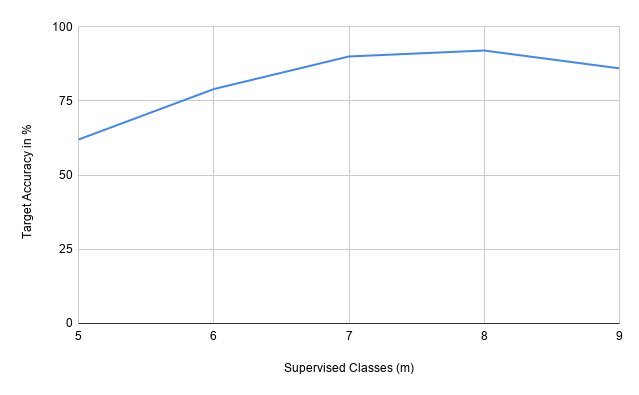
\includegraphics[width=0.8\textwidth]{abbildungen/mixedResults.png}
  \caption{Results of the experiments with the DSN': Target accuracy of the DSN' with all losses activated when trained $m$ supervised classes from $S$ and $M$.}
  \label{dia:mixedDSN}
\end{figure}

\begin{figure}[tbh]
  \centering
    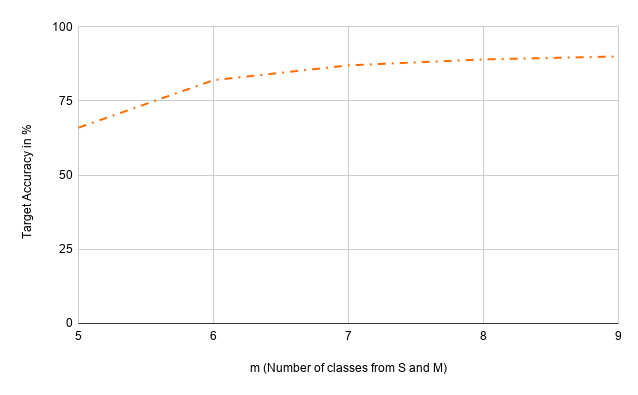
\includegraphics[width=0.8\textwidth]{abbildungen/mixeddaResults.png}
    \caption{Results of the experiments with the DSN' sim: Target Accuracy of the DSN' with only similarity loss activated trained on $m$ supervised classes from $S$ and $M$. This setup has a similar architecture to DANN.}
  \label{dia:mixedDA}
\end{figure}

\paragraph*{Discussion} Our results confirm the observation made in \cite{domainMixture} regarding the quasi constant performance of the model when it uses domain adaptation on the mixed domains. This also proves the architecture's ability to extract domain-free representations with which the classifier can train effectively even when multiple domains are present and the domains are incomplete.

However, a remarkable notice is, in our setup, the performance gap between training on a domain with 5 supervised classes from each domain and training with 6 classes per domain. On one hand, this should not be surprising since more supervised data offers more information and having more supervised classes resembles traditional machine learning that needs no domain adaptation. On the other hand, we have seen that the model can cope well with missing domain-class representation for $m \geqslant 6$ but performs unproportionally worse when $m=5$. After considering the differences between the architecture and the setups, we propose these possibilities to answer for this behavior:

\paragraph*{Overfitting} As we know, learning repeatedly on the same data for too much could make the network memorizes the training and therefore inhibits its ability to generalize the task to the unknown data. As we chose to train the network with an equal number of update step for all the number of classes $m$ within the same setup, the variation with only 5 supervised domains would offer the least amount of data among them and could therefore cause overfitting. To check this possibility, we evaluate the model at earlier training stages, i.e., as less learning steps have been made. The earlier performances on these steps also show no significant signs of overfitting, they perform partly equivalent and partly worse than the end results shown above. Therefore, the evidences seem not to point to overfitting as the cause of this behavior. 

\paragraph*{Randomly Assembled Batches} After negating the overfitting as the cause of this performance gap, we look for a difference between our experiments and those in \cite{domainMixture}. A difference we regard as a possible cause is how we generate batches for the gradient descent. In \cite{domainMixture}, they explicitly generate batches with half supervised samples and half unsupervised. Hence, the classifier has something to train on in every steps equally to the domain classifier can learn about the domains. In our experiments, we generate the batches by randomly choose the data in the mixed domains. It is therefore possible that the classifier did not trained equally well in each step and might be still underdeveloped or developed in the sub-optimal way. Ideally, the experiments should be repeated with similarly generated batches to observe the results. We consider this to be an open question requiring further studies. 

\paragraph*{Reaction of the DSN to lack of Overlapping Supervised Classes} Another speculation to explain this behavior is that the DSN reacts differently on the extra overlapping domain-class combinations offered in cases of $m \geqslant 6$. We call this a speculation because there is no obvious reason regarding the architecture. Only the similarity loss activated, the DSN actually includes the same mechanisms as the DANN in that it learns adversarially with the gradient reversal layer and the classifier is feed only with representations created from the shared encoders. A confusion matrix similar to that in \cite{domainMixture} could be calculated to see what kind of false predictions were being made. Whether it uses the different domain to make assumption about the classes that one domain could not include those classes it only has seen in another domain in the training. This possibility needs to be further investigated to understand this behavior better. \\

\begin{figure}[tbh]
  \centering
    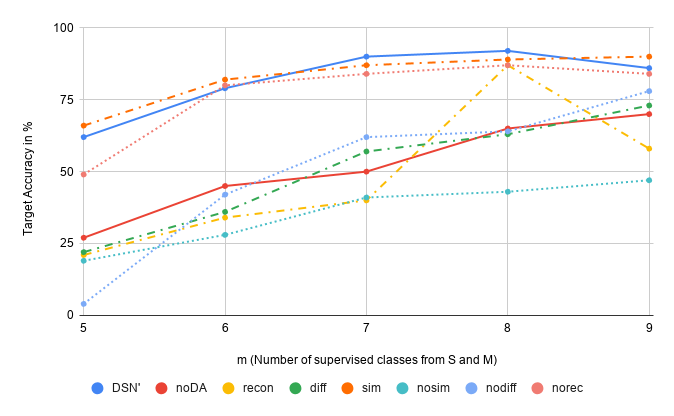
\includegraphics[width=0.8\textwidth]{abbildungen/allDSNResults.png}
    \caption{Results of all the DSN' setups: Target Accuracy of all the DSN' variations experimented on the complete domain mixture scenario with different mixture combinations out of $m$ supervised classes from both $S$ and $M$.}
  \label{fig:allDSNResults}
\end{figure}

To see the impacts of each different losses on the performance of the DSN, the experiments were also carried with different loss combinations. All the combinations tested and their abbreviation used in this thesis are listed in Table \ref{tb:lossCombinations} in Section \ref{sec:exSetups}. The target accuracies of all the settings are plotted in Figure \ref{fig:allDSNResults}.

The worst average performance is delivered when the similarity loss is deactivated, as seen in the 'nosim' case. The DSN' makes overall even more inaccurate prediction with this loss combination than without any loss activated - the no domain adaptation 'noDA' case. This may result from the constraints put on the networks through other activated losses while the classifier already has to train on the domain-contaminated representations - the similarity loss responsible for the domain-independent shared representations is deactivated and the other losses further complicate the optimization problem. An evidence supporting this argument is that other setups such as 'recon' and 'diff' which are also trained without the similarity loss perform better quasi overall better with only one other loss activated. 

Another interesting point is the peak performance at $m = 8$ of the 'recon' setup with only reconstruction loss activated. At $m = 8$, the DSN' with this setup has an almost constant target accuracy of 86\%, even better than at $m = 9$. It is possible that these good results could be only straying outliers. With the existing data, this possibility cannot be eliminated, further runs with this setup should be executed again. A conclusion that $m = 8$ is the 'golden spot' of this setup cannot be made yet since there is no supporting argument. 

It is also clear to see that the similarity loss has the most impact on the target accuracy of the setups. All the combinations with this loss deactivated perform significantly worse than those with this loss activated. The differences between these combinations seem to decrease with more supervised data. The strong dependence of the performance on the similarity loss is understandable because the similarity loss is the key to creating domain-irrelevant representations on which the classifier can train to perform domain transfer at its best according to a theory of domain adaptation. Other losses, the reconstruction loss and the difference loss, seem to be complementary to the similarity loss.

On the contrary, deactivating only reconstruction loss appears to affect the performance of the DSN' only minimally. This setup, referred to as 'norec', performs only slightly worse than the setup with all losses activated (DSN') and with only similarity loss activated (sim). 

The last remarkable insight seen in the graph is the significantly low accuracy of only 4\% of the 'nodiff' DSN' at $m = 5$. As mentioned above, removing the similarity highly affects the performance. However, the average performance of this particular setup is significantly low. In many runs with this setup, the accuracy is almost 0 whereas some of them even reach 30\%. Since $m = 5$ offers less information, it is imaginable that overfitting could be the cause. A look on the recorded target accuracy over the training phase, however, indicates no clear signs of overfitting or anomaly in the training. The target accuracy seems to normally converge against 0. This high variance in the performance among the same setup and the significantly low performance at $m=5$ should be studied further. For this, a confusion matrix, for instance, could also offer useful information on this behavior similar to the aforementioned problem of the performance gap.

Generally, these bad results and unstable results, i.e., big differences in performance between runs, can also be observed in many setups with $m = 5$ or $m = 6$ . The model apparently trains more stably and more effectively with more supervised data. 

 There are more potential works to be done which unfortunately cannot be included into this thesis due to time restriction. For example, the investigation of the performance gap, the significantly low performance and the unstable performances between runs should be carried further. Further studies on the influences of different losses on the performance of the network could be useful in designing further architectures inspired from these different parts of the DSN. 


\chapter{Conclusion} \label{ch:conclusion}
With increasing popularity of deep neural networks, data collection has become more crucial at the same time. Fortunately, the internet and the new technologies allow us to collectively share our data over the world and over time. For computer vision, new camera models and those coming with mobile phones allow even more possibilities to capture images all the time and all over the places, which many of us also do. With all the data coming in, explicitly collecting data can be limited if, and only if, we can make use of this data. As already studied, using these images of different natures without taking their diversities into account are not effective and could make things worse. This possibility of using existing data or trained networks motivates the development of domain adaptation methods to optimize this opportunity. 

Many theories and networks are already created to apply this method to real problems. Mostly, however, the scenarios investigated involve adapting one domain to another, which represents the reality only limitedly. The images in the real world come from many different conditions and capturing methods. Even doing researches, the datasets previously collected each have their own biases. Only assuming that there will be only one domain in the training dataset is not realistic and even lead to sub-optimal performance. For example, some methods applying domain adaptation do not account for the different distributions of the domains and if existing domains are all treated as one training domain, these differences do not fully support the adaptation as it could be. Though still a minority, there are also studies on domain adaptation with multiple sources which describe the problem more realistically. They propose methods accounting for the existing diversity in the source domain to allow for better knowledge extraction which results in better domain adaptation at the end. 

Another still overlooked scenario in domain adaptation is also when there are many domains acting as a source domain and they are not complete, i.e., they do not have representations of all the classes that should be classified. This situation is even nearer to the reality since we cannot expect all image sources to have the same kinds of image and all the types of object we want. By trying to classify more and more objects, it is plausible to assume that more and more data source will have to be merged to cover all the target objects. 

In this thesis, we focused our work on a specific case of this scenario, the complete domain mixture scenario. The theories on the neural networks, domain adaptation and the involving problems are introduced for better understanding of the experiments. Also, in addition to the theoretical explanation, examples of the real usages or previous studies were integrated to bring the practicality into the theories. Then, the experiments on this scenario were carried with the domain separation network, a network proposed to tackle the domain adaptation by leaning to extract the domain information in order to learn the object information independently. Based on the results presented in \cite{DSN} and \cite{domainMixture}, interesting insights that need further inspections were found. The performance of the DSN' without the similarity loss is noticeably lower than when the loss is activated which further confirms the effectiveness of the domain-free representations in applying domain adaptation. On the other hand, the reconstruction loss and the difference loss seem to be complementary to the similarity in making better representations without contamination from the domain aspects of the inputs. Theses losses, when activated solely, offer averagely the same accuracy as if no domain adaptation is applied in the complete domain mixture scenario. Furthermore, the DSN' presents a performance gap in this scenario between supervised classes $m = 5$ and $m = 6$. Since overfitting seems, at least at first glance, not to be the cause, further investigation is still needed. The experiments should be repeated again with training batches containing equal amount of supervised and unsupervised data to ensure a constant training of the classifier. Also, the unstable results between runs with the same setups when less supervised images are involved i.e. $m \leq 6$, can be observed. Partly, the accuracy is close to 0. Possible reasons of this should also be validated. The confusion matrix, for instance, can be calculated to gain more information about the wrong predictions.

The complete domain mixture scenario is only a special case of the domain mixture scenario. Conditioned to offer the data for all the competing classes, the training is simplified since the system has 'seen' all types of objects under every involving domains even if the information is not supervised. Another special condition are only partly supervised domains. In the reality, it is possible that some of the domains are either fully supervised or lack completely of data on particular objects. Generally, the domain mixture scenario is highly related to the real-world situations. The completeness and incompleteness of the datasets cannot always be predicted or ordered as will. So far to the best knowledge, there are still significantly less works done similarly on the scenarios with mixed domains than on those with complete domains. Therefore, it is encouraged to study this scenario more to better understand of the reality and its potential use. The opportunity to use the data under this particular scenario is huge and will be worth the work. 
% HIER WEITERE ABSCHNITTE EINFÜGEN


%\appendix			% schaltet Umgebunsvariablen um auf Anhang
%\input{appendix1}		% erster Teil des Anhangs (wird eher selten benötigt)

\backmatter			% Literaturverzeichnis, Index usw.

%%%%%%%%%%%%%%%%%%%%%%%%%%%%%%%%%%%%%%%%%%%%%%%%%
% Literatur
%%%%%%%%%%%%%%%%%%%%%%%%%%%%%%%%%%%%%%%%%%%%%%%%%
\begingroup
\raggedright\sloppy
\bibliography{Literatur}		% Name der *.bib Datei in der die Literatur steht
\endgroup
%nocite{*}						% Auflisten aller Quellen, auch wenn diese nicht in der Arbeit zitiert sind

% Stil des Literaturverzeichnis (nach DIN1505)
%\bibliographystyle{unsrtdin} % sortiert nach Reihenfolge im Text mit Nummern
\bibliographystyle{plaindin} % alphabetisch sortiert mit Nummer
%\bibliographystyle{alphadin} % alphabetisch sortiert mit Autor-Jahr-Kürzel statt Nummer

\end{document}
